% Version 0; preprint format; Written by SH
% Version 1; emulateapj format; Edited by SH and AL
% Version 2; emulateapj format; Edited by SH and AL
% Version 3; emulateapj format; Edited AL
% Version 4; emulateapj format; Edited SH
% Version 5; MNRAS format; Edited SH
% Version 6; MNRAS format; Paper I edited by JG
% Version 7; MNRAS format; Edited by SH

\documentclass[a4paper,fleqn,usenatbib]{mnras}

% Packages
\usepackage{deluxetable}
\usepackage{newtxtext,newtxmath}
\usepackage[T1]{fontenc}
\usepackage{ae,aecompl}
\usepackage{amssymb, amsmath}
\usepackage{graphicx}
\usepackage{natbib}
\usepackage{url}
\usepackage{hyperref}
\usepackage{float}
\usepackage[usenames, dvipsnames]{color}

% Package Settings
\hypersetup{colorlinks=true,
            citecolor=MidnightBlue,
            linkcolor=MidnightBlue,
            filecolor=magenta,      
            urlcolor=cyan}
\urlstyle{same}

% Figure extention
\DeclareGraphicsExtensions{.pdf,.png,.jpg}

%%%%%%%%%%%%: User Defined Commands %%%%%%%%%%%%

% Song Huang's definition 
\def\arcsec{{\prime\prime}}
\def\arcmin{{\prime}}
\def\degree{{\circ}}
\def\h{\hskip -3 mm}
\def\aa{{A\&A}}
\def\aas{{ A\&AS}}
\def\aj{{AJ}}
\def\al{$\alpha$}
\def\bet{$\beta$}
\def\amin{$^\prime$}
\def\annrev{{ARA\&A}}
\def\apj{{ApJ}}
\def\apjs{{ApJS}}
\def\asec{$^{\prime\prime}$}
\def\deg{$^{\circ}$}
\def\ddeg{{\rlap.}$^{\circ}$}
\def\dsec{{\rlap.}$^{\prime\prime}$}
\def\cc{cm$^{-3}$}
\def\flamb{erg s$^{-1}$ cm$^{-2}$ \AA$^{-1}$}
\def\flux{erg s$^{-1}$ cm$^{-2}$}
\def\fnu{erg s$^{-1}$ cm$^{-2}$ Hz$^{-1}$}
\def\hst{{\textit{HST}}}
\def\kms{km s$^{-1}$}
\def\lamb{$\lambda$}
\def\lax{{$\mathrel{\hbox{\rlap{\hbox{\lower4pt\hbox{${\sim}$}}}\hbox{$<$}}}$}}
\def\gax{{$\mathrel{\hbox{\rlap{\hbox{\lower4pt\hbox{${\sim}$}}}\hbox{$>$}}}$}}
\def\simlt{\lower.5ex\hbox{$\; \buildrel < \over {\sim} \;$}}
\def\simgt{\lower.5ex\hbox{$\; \buildrel > \over {\sim} \;$}}
\def\micron{{$\mu$m}}
\def\mnras{{MNRAS}}
\def\nat{{Nature}}
\def\pasp{{PASP}}
\def\perang{\AA$^{-1}$}
\def\peryr{yr$^{-1}$}
\def\reference{\noindent\pp}
\def\refindent{\par\noindent\parskip=2pt\hangindent=3pc\hangafter=1 }
\def\sb{mag~arcsec$^{-2}$}
\def\lsun{$L_\odot$} 
\def\msun{$M_\odot$}
\def\sigs{$\sigma_*$}
\newcommand{\lt}{<}
\newcommand{\gt}{>}

\def\etal{{\ et al.~}}
\def\galfit{{\tt GALFIT}}
\def\ser{{S\'{e}rsic\ }}
\def\redm{\texttt{redMaPPer}}
\def\cmodel{\texttt{cModel}}
% Samples
\def\rbcg{\texttt{cenHighMh}}
\def\nbcg{\texttt{cenLowMh}}
\def\redbcg{{$\lambda \ge 30$}}
\def\nonbcg{{$\lambda < 20$}}
% Mass related 
\def\mstar{{$M_{\star}$}}
\def\mhalo{{$M_{\mathrm{halo}}$}}
\def\logms{{$\log (M_{\star}/M_{\odot})$}}
\def\logmh{{$\log (M_{\mathrm{halo}}/M_{\odot})$}}

\def\minn{{$M_{\star,10\mathrm{kpc}}$}}
\def\meff{{$M_{\star,15\mathrm{kpc}}$}} 
\def\mtot{{$M_{\star,100\mathrm{kpc}}$}}
\def\mout{{$M_{\star,150\mathrm{kpc}}$}}
\def\mmax{{$M_{\star,\mathrm{Max}}$}}
\def\mgama{{$M_{\star,\mathrm{GAMA}}$}}
\def\mcmodel{{$M_{\star,\mathrm{cModel}}$}}

\def\logminn{{$\log (M_{\star,10\mathrm{kpc}}/M_{\odot})$}}
\def\logmtot{{$\log (M_{\star,100\mathrm{kpc}}/M_{\odot})$}}
\def\logmout{{$\log (M_{\star,150\mathrm{kpc}}/M_{\odot})$}}
\def\logmmax{{$\log (M_{\star,\mathrm{Max}}/M_{\odot})$}}
\def\logmgama{{$\log (M_{\star,\mathrm{GAMA}}/M_{\odot})$}}
\def\logmcmodel{{$\log (M_{\star,\mathrm{cModel}}/M_{\odot})$}}

\def\m2l{{$M_{\star}/L_{\star}$}}
\def\mden{{$\mu_{\star}$}}

% Commenting:
\newcommand{\xxx}[1]{\textcolor{red}{\textbf{XXX}}}
\newcommand{\todo}[1]{\textcolor{red}{\textbf{TODO:~#1}}}
\newcommand{\plan}[1]{\textcolor{cyan}{#1}}
\newcommand{\addref}{{\textcolor{red}{REF}}}
\newcommand{\note}[2]{\textcolor{blue}{\textbf{[Comment (#1): #2]}}}
\newcommand{\song}[1]{\textcolor{magenta}{\textbf{[Song: #1]}}}
\newcommand{\alexie}[1]{\textcolor{blue}{\textbf{[Alexie: #1]}}}
\newcommand{\jenny}[1]{\textcolor{Bittersweet}{\textbf{[Jenny: #1]}}}
\newcommand{\kevin}[1]{\textcolor{green}{\textbf{[Kevin: #1]}}}
\newcommand{\update}[1]{\textcolor{PineGreen}{#1}}
%\newcommand{\update}[1]{#1}


%%%%%%%%%%%%: Title and Affiliations %%%%%%%%%%%%

%% ------------------------------------------------------------------------------------ %% 
\title[Mass Dependent Stellar Halo in Massive Galaxies]{Tracing the Stellar Halo of 
	   Massive Galaxies to 100 kpc at $0.3<z<0.5$ using the Hyper Suprime-Cam}

\author[S. Huang et al.]{
        Song Huang,$^{1,2}$\thanks{E-mail: song.huang@ipmu.jp (SH)}
        Alexie Leauthaud,$^{2,1}$
        Jenny E. Greene,$^{4}$
        Kevin Bundy,$^{3,1}$
        \newauthor
        Yen-Ting Lin,$^{5}$
        Masayuki Tanaka,$^{5}$
        Rachel Mandelbaum,$^{7}$
        Satoshi Miyazaki,$^{5,8}$
        \newauthor
        Yutaka Komiyama,$^{5,8}$
        HSC collaboration 
        \\
        $^{1}$Kavli-IPMU, The University of Tokyo Institutes for Advanced Study, 
              the University of Tokyo (Kavli IPMU, WPI), Kashiwa 277--8583, Japan\\
        $^{2}$Department of Astronomy and Astrophysics, University of California 
              Santa Cruz, 1156 High St., Santa Cruz, CA 95064, U.S.A\\
        $^{3}$UCO/Lick Observatory, University of California, Santa Cruz,
              1156 High Street, Santa Cruz, CA 95064, USA\\
        $^{4}$Department of Astrophysical Sciences, Peyton Hall,
              Princeton University, Princeton, NJ 08540, USA \\
        $^{5}$National Astronomical Observatory of Japan, 2--21--1 Osawa, Mitaka, 
              Tokyo 181--8588, Japan\\
        $^{6}$Academia Sinica Institute of Astronomy and Astrophysics, 
              P.O. Box 23--141, Taipei 10617, Taiwan\\
        $^{7}$McWilliams Center for Cosmology, Department of Physics, 
              Carnegie Mellon University, Pittsburgh, PA 15213, USA\\
        $^{8}$SOKENDAI (The Graduate University for Advanced Studies), Mitaka,
              Tokyo, 181--8588, Japan
        }   
%% ------------------------------------------------------------------------------------ %% 
\date{Accepted XXX. Received YYY; in original form ZZZ}        
\pubyear{2017}                                  
  
%%%%%%%%%%%%: Header and Version %%%%%%%%%%%%
\begin{document}

\label{firstpage}
\pagerange{\pageref{firstpage}--\pageref{lastpage}}

\maketitle

%%%%%%%%%%%%: Abstract and Keywords %%%%%%%%%%%%

\begin{abstract} 
    
    Massive galaxies are important to our understanding of galaxy formation, and 
    their extended stellar halos contain crucial fossil records of their assembly 
    history. 
    In this work, we use ${\sim}100$ deg$^2$ of deep ($>28.5$ \sb{} in $i$-band), 
    high-quality (0.6\asec seeing) imaging data from the Hyper Suprime-Cam (HSC) 
    survey to investigate the surface mass density profiles and outer stellar halos 
    of massive galaxies. 
    Our sample consists of ${\sim}7000$ massive (\mstar{}$\geq 11.5$) central galaxies 
    at $0.3 < z < 0.5$. 
    The depth of the HSC survey reaches ${\sim}4$ magnitudes fainter than SDSS and 
    enables us to directly trace stellar mass distributions to 100 kpc without 
    requiring stacking. 
    Shallow images and/or over-simplified models like the \texttt{CModel} tend to 
    miss the extended stellar halo and result in underestimated stellar mass in a 
    mass-dependent way.  
    It will impact important applications like the measurements of the stellar mass 
    function. 
    With these deeper data, we explicitly show that at fixed stellar mass,
    massive central galaxies display surface mass density profiles that are not 
    self-similar, with the outer-slope becoming shallower and the fraction of mass 
    in the outskirt increasing with total stellar mass.
    We also show that the ellipticity of the stellar halo increases with stellar
    mass, while the optical color gradients do not strongly depend on stellar mass.
    Our results are broadly consistent with the two phase formation scenario of 
    massive galaxies in which outer envelopes are built up at late times from the 
    accretions of small systems. 
    The surface mass density profiles are provided in a convenient tabulated format 
    in order to facilitate comparisons with predictions from numerical simulations 
    of galaxy formation.
           
\end{abstract}

\begin{keywords}
    galaxies: elliptical and lenticular, cD --
    galaxies: formation --
    galaxies: photometry -- 
    galaxies: structure -- 
    galaxies: surveys
\end{keywords}


%%%%%%%%%%%%: Main Text %%%%%%%%%%%%

%% ------------------------------------------------------------------------------------ %% 
    \begin{figure*}
        \centering 
        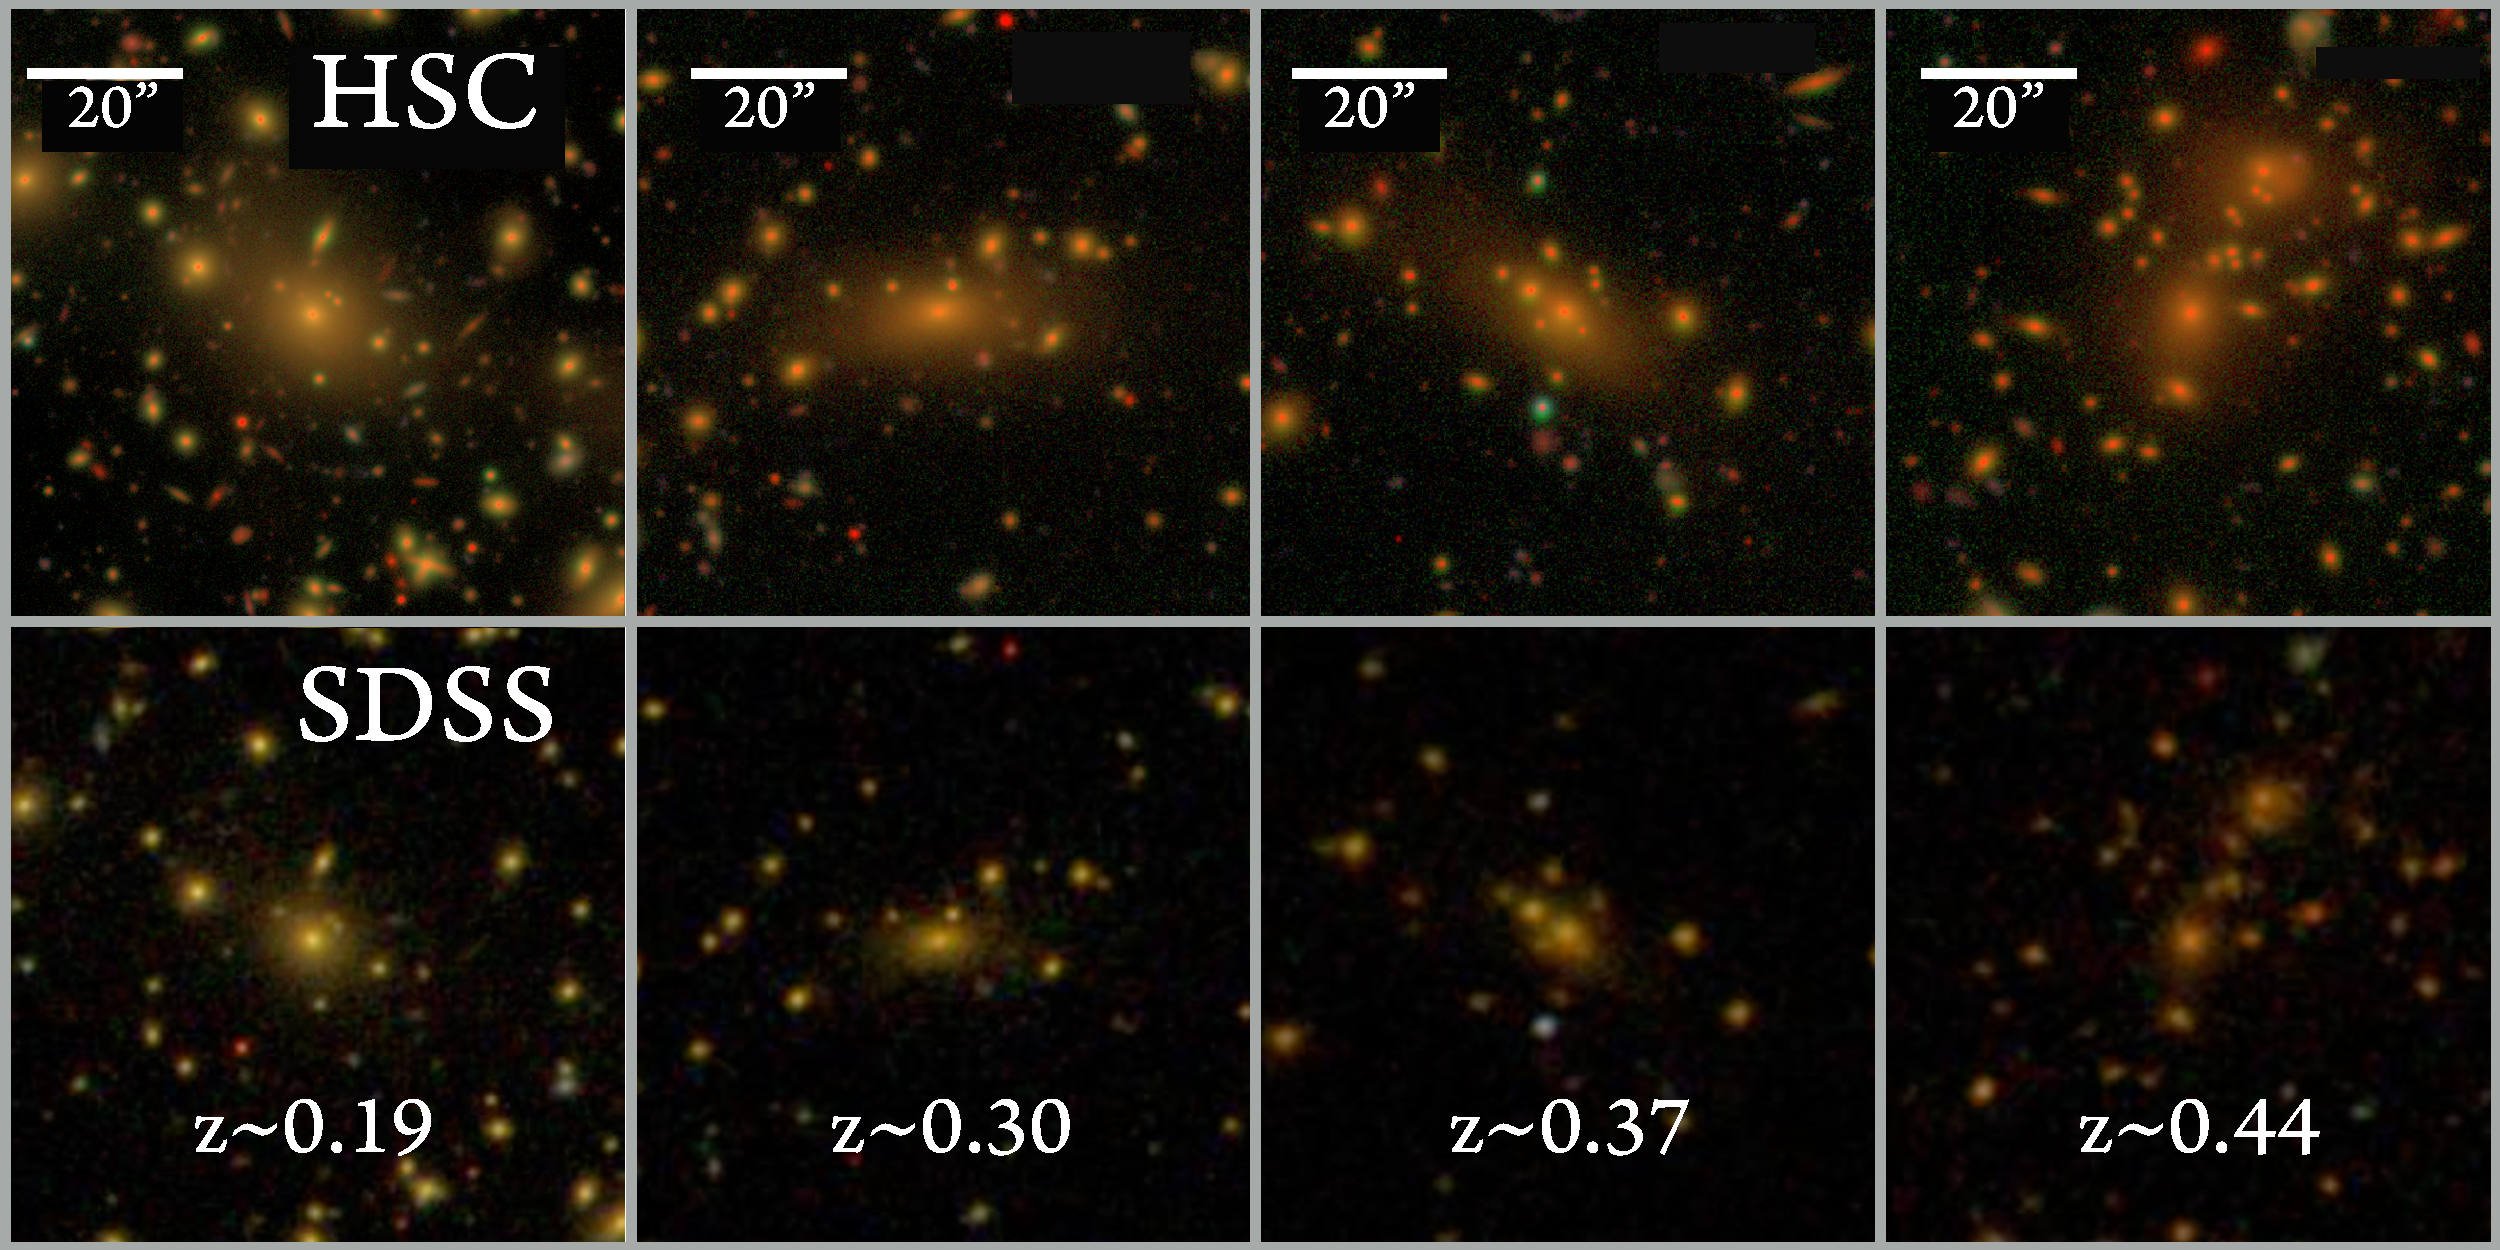
\includegraphics[width=\textwidth]{fig/redbcg_sdss_compare}
        \caption{
            A comparison between the depth and imaging quality of SDSS and the HSC wide 
            layer for a sample of nearby massive elliptical galaxies at $0.2 < z < 0.5$.  
            These images are generated using $gri$ band images with an arcsinh stretch 
            \citep{Lupton2004}. 
            The HSC \texttt{WIDE} layer is $3.0$-$4.0$ magnitudes deeper than SDSS.
            This added depth is critical in order map the outskirts of ETGs out to 
            large radii.
            }
        \label{fig:sdss_compare}
    \end{figure*}
%% ------------------------------------------------------------------------------------ %% 

%% ------------------------------------------------------------------------------------ %% 
\section{Introduction}
    \label{sec:intro}

    Massive galaxies are fascinating objects that have experienced complex assembly 
    process and dramatic evolution.  
    They are crucial for both cosmology and the study of galaxy formation. 
    Simulations of structure formation within the context of the $\Lambda$-CDM 
    cosmological model make predictions for the hierarchical growth of dark matter 
    halos and galaxies (e.g. \citealt{Baugh1996, DeLucia2006}), but there are many 
    open questions regarding the star-formation history, mass assembly process, and 
    structural evolution of massive galaxies. 
    Massive galaxies are thought to grow according to a ``two-phase'' formation 
    scenario (e.g. \citealt{Oser2010, Oser2012}). 
    In this scenario, the progenitors of $z{\sim} 0$ massive early-type galaxies 
    (ETGs) undergo a rapid growth phase at $z{\sim} 2$ triggered either by disk 
    instabilities or gas-rich mergers (e.g. \citealt{Hopkins2008, Dekel2009}). 
    Observationally, the progenitors of ETGs are thought to correspond to the 
    population of massive quiescent galaxies at high redshift that have smaller 
    average effective radii ($R_{\mathrm{e}}$; e.g. \citealt{Trujillo2006, 
    vanDokkum2008, Cimatti2008}), slightly higher central velocity dispersion and 
    stellar mass density (\mden{}; e.g. \citealt{vandeSande2011, Belli2014}), and 
    more disk-like morphologies (e.g. \citealt{vanderWel2011}) than their local 
    descendants (e.g. \citealt{Bezanson2009, vanDokkum2010}) with similar stellar 
    mass.
    
    Following this initial epoch of early formation, feedback from stars and/or AGN 
    (e.g. \citealt{Sijacki2007, Fabian2012}) efficiently quench star formation in 
    massive galaxies. 
    A large fraction of these massive progenitors became quiescent at $z>1$ 
    (e.g. \citealt{Bezanson2009, Kriek2016}). 
    The second phase of their assembly is driven by non-dissipative processes such 
    as dry mergers with other galaxies (e.g. \citealt{Naab2006, Khochfar2006}). 
    To explain the observed increase of $R_{\mathrm{e}}$ (e.g. 
    \citealt{Newman2012, vdWel2014}) as well as the build-up of the outer stellar 
    halos of ETGs (e.g. \citealt{Szomoru2012, Patel2013}), the ``two-phase'' 
    scenario suggests that minor mergers should dominate the mass assembly during 
    the second phase (e.g. \citealt{Hilz2012, Hilz2013, Oogi2013, Bedorf2013, 
    Laporte2013}).
    Both numerical simulations (e.g. \citealt{Oser2010}) and 
    semi-analytic models (SAM; e.g. \citealt{LeeYi2013, LeeYi2017}) agree that the 
    mass fraction in the accreted component should increase with total stellar mass, 
    despite their technical differences (e.g. \citealt{Lackner2012, Cooper2013, 
    Qu2017}).
    For instance, recent result from the Illustris \footnote{
    \texttt{http://www.illustris-project.org/}} simulation 
    (\citealt{Vogelsberger2014}, \citealt{Genel2014}) predicts that the fraction of  
    accreted stars increases significantly with total stellar mass at \logms{}$>11.0$, 
    and the accreted component starts to dominate the stellar mass budget 
    ($f_{\mathrm{accreted}}>0.5$) at \logms{}$>11.5$ (\citealt{RodriguezGomez2016}).
%% ------------------------------------------------------------------------------------ %% 
    
    Given the success of this two-phase scenario in explaining trends like overall size 
    growth, it is time to confront their predictions with additional observations, 
    especially the detailed profiles of surface mass density and shape for low redshift 
    massive galaxies.  
    Early one-dimensional analysis of nearby massive ETGs suggest that the 
    single-\ser{} profile can describe their surface brightness (or surface mass 
    density) profiles reasonably well (e.g. \citealt{Kormendy2009}; except for the
    most central region), with the \ser{} index increasing with total luminosity 
    (e.g. \citealt{Graham2013}).
	However, the situation is in fact more complicated, with a suggestion from 
	\citet{Schombert2015} that there are actually two families of light profiles:
	the ones that follow single-\ser{} law well and the ones show significant 
	deviation.
	Two-dimensional analysis, meanwhile, finds that the stellar distributions 
    of massive ETGs are often better fit by multiple-component models 
    (e.g. \citealt{Huang2013a, Oh2017}). 
    \citet{Huang2013b} further suggests a connection between the multi-component 
    nature of massive galaxies and their two-phase assembly history. 
    To further confront the two-phase scenario requires very deep observations of 
    large samples of massive ETGs to correctly estimate their total stellar mass 
    (e.g. \citealt{Bernardi2013, DSouza2014}) and explore their assembly history via 
    their extended, accreted halos (e.g. \citealt{Capaccioli2015, Iodice2016, 
    Iodice2017}).
    Currently, such work is limited by the depth of imaging from large-area surveys 
    such as the Sloan Digital Sky Survey (SDSS; e.g. \citealt{SDSSDR7, SDSSDR12}) or
    the small sample size of massive galaxies with deep images.  
    
    In this paper, we take advantage of new high-quality (median 
    FWHM${\sim} 0.6^{\arcsec}$ in $i$-band) and deep ($i$-band surface brightness 
    limit $> 28.5$\sb) images from the Hyper Suprime-Cam (HSC) Subaru Strategic 
    Program \citep[SSP,][]{HSCDR1} to characterize the outer parts of massive galaxies 
    as a function of their properties. 
    The deep imaging depth and excellent seeing conditions of HSC images make them 
    perfect for mapping the \mstar{} distributions of massive galaxies out to very 
    large radii. 
    With the help of reliable spectroscopic and photometric redshift 
    (e.g. the ones for \redm{} clusters, \citealt{Rykoff2014}; \citealt{Rozo2015b}),
    we select a large sample (${\sim} 7000$) of massive central galaxies at 
    $0.3 < z < 0.5$ using ${\sim} 100$ deg$^2$ of data from the HSC wide layer. 
    In this paper, we use this sample to 
    (a) reliably measure individual surface mass density (\mden{}) profile of 
    massive galaxy out to 100 kpc, 
    (b) investigate the dependence of their outer stellar halos on total stellar 
    mass, and 
    (c) examine the implications for the stellar mass function (SMF) when the outer 
    halos of massive galaxies are accounted for.   
    In a second paper in this series, we will further look into the potential 
    environmental dependence of structures in massive ETGs (Huang\etal in prep.).
    
    This paper is organized as follows. 
    Section \ref{sec:data} presents our data and our sample selection. 
    Section \ref{sec:ellipse} describes our procedure for extracting 1-D surface 
    brightness profiles. 
    Section \ref{sec:mstar} describes how we estimate stellar mass. 
    Our main results are presented in Section \ref{sec:result} and discussed in 
    Section \ref{sec:discussion}. 
    Section \ref{sec:summary} presents our summary and conclusions.

    Magnitudes use the AB system (\citealt{Oke1983}), and are corrected for Galactic 
    extinction using calibrations from \citet{Schlafly11}.
    In this work, we assume $H_0$ = 70~km~s$^{-1}$ Mpc$^{-1}$, ${\Omega}_{\rm m}=0.3$, 
    and ${\Omega}_{\rm \Lambda}=0.7$.
    Stellar mass is noted \mstar{} and has been derived using a Chabrier Initial Mass 
    Function (IMF; \citealt{Chabrier2003}).   
      
    $M_{\mathrm{halo}}$ denotes halo mass in general whereas $M_{\rm 200b}$ is 
    explicitly defined as $M_{\rm 200b}\equiv M(<r_{\rm 200b})=200\bar{\rho} 
    \frac{4}{3}\pi r_{\rm 200b}^3$ where $r_{\rm 200b}$
    is the radius at which the mean interior density is equal to 200 times
    the mean matter density ($\bar{\rho}$). 
    
%% ------------------------------------------------------------------------------------ %% 

%% ------------------------------------------------------------------------------------ %% 
    \begin{figure*}
        \centering 
        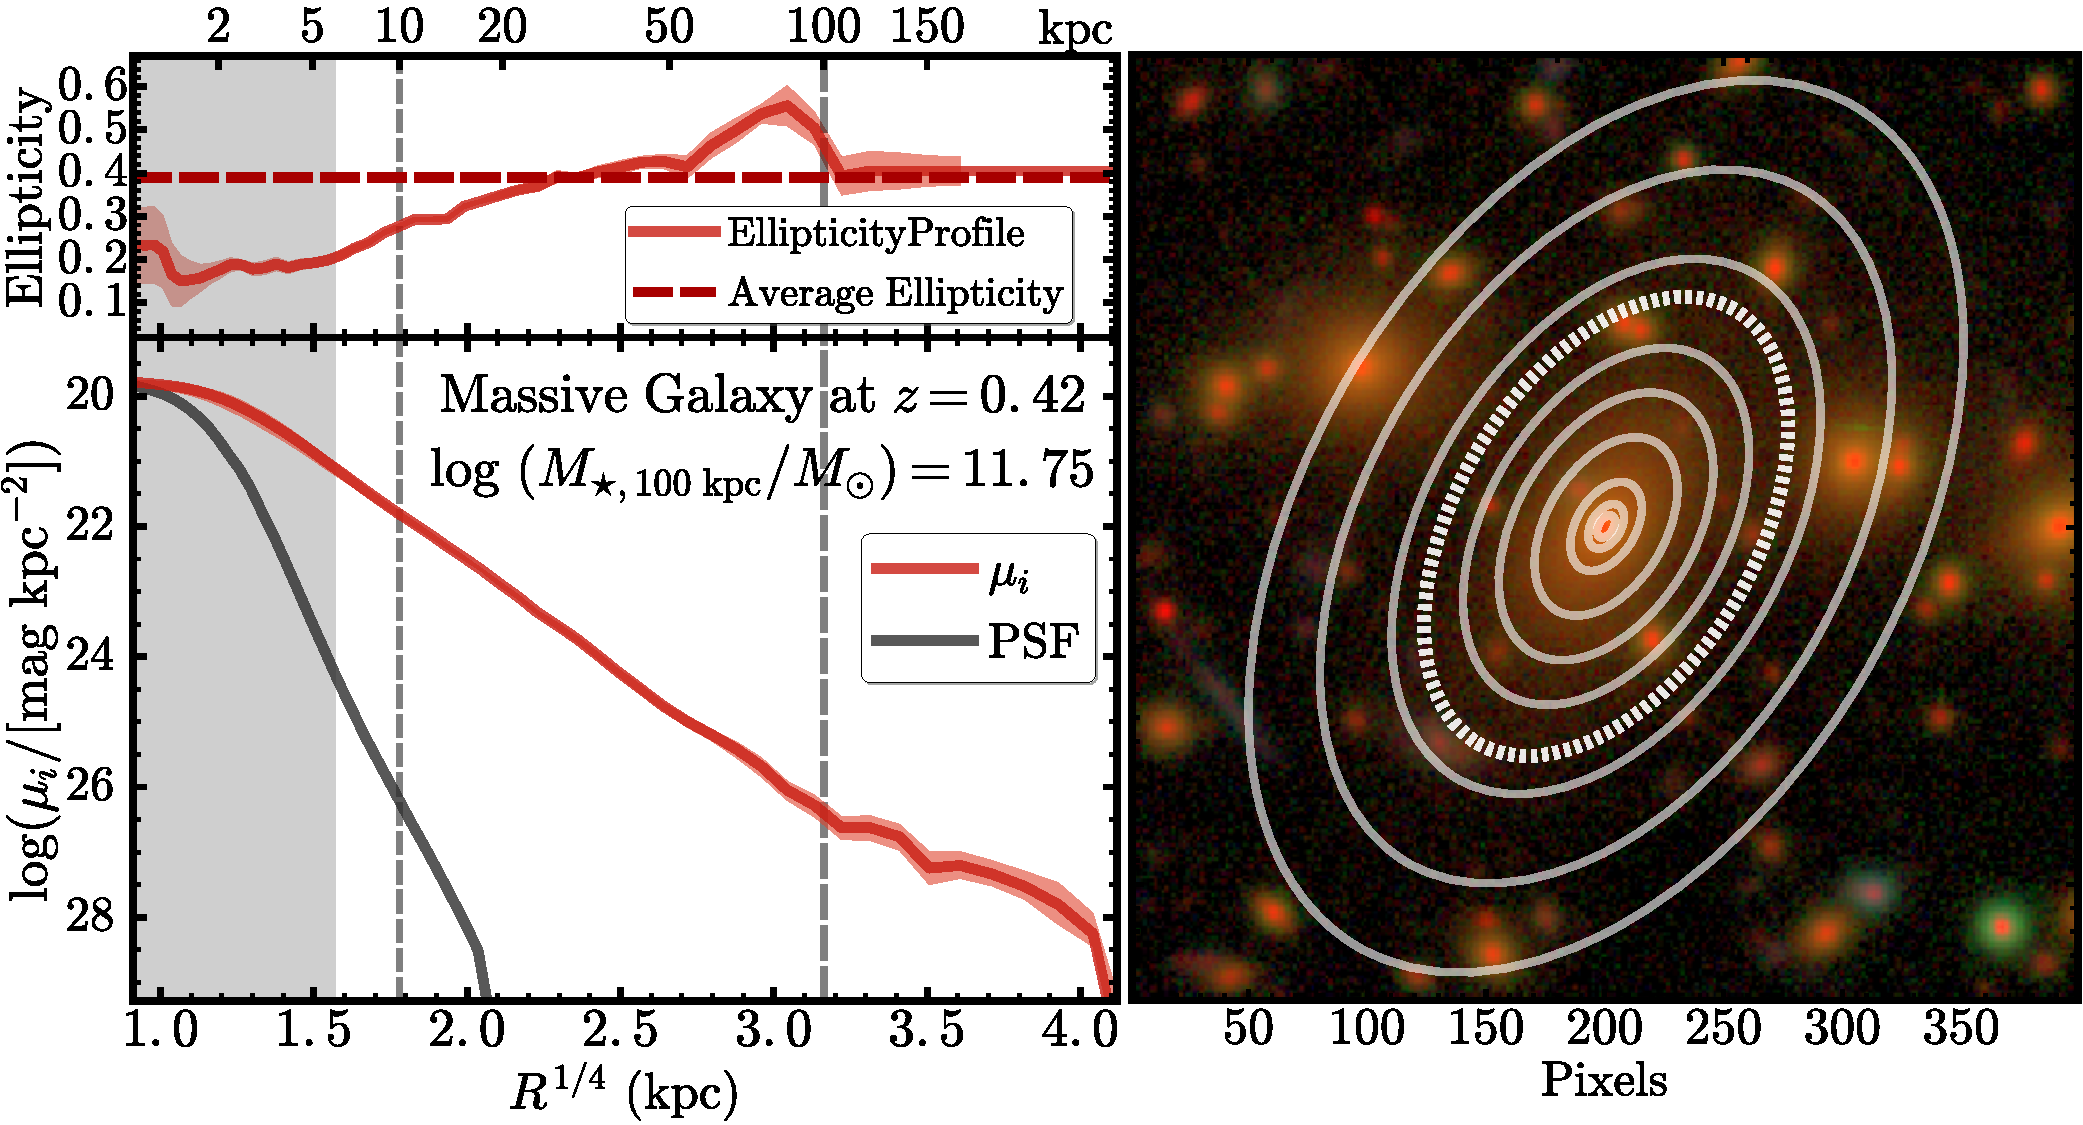
\includegraphics[width=\textwidth]{fig/redbcg_ellipse_example}
        \caption{
            Left: example of the 1-D surface brightness and ellipticity profile 
            for a massive galaxy at $z=0.23$ in the $i$-band using \texttt{Ellipse}. 
            In this work, we always show the radial profile using a $R^{1/4}$ scaling 
            on the x-axis. 
            By using this scale, the de Vaucouleurs profile will appear as a straight 
            line on this figure. 
            We also plot the relative brightness profile of the PSF model normalized 
            at the central surface brightness of the galaxy to highlight the region 
            affected by seeing. 
            The grey shaded region highlights the region most affect by seeing 
            ($r<3$ kpc).
            On the top panel, the dash line shows the ellipticity used for the final 
            isophote. 
            Right: the three color image of this galaxy with isophotes 
            extracted by \texttt{Ellipse}. 
            The thick dotted line highlights the isophote with 
            $\mu_{i}{\sim} 28.5$~\sb.
            }
        \label{fig:ellipse}
    \end{figure*}
%% ------------------------------------------------------------------------------------ %% 

%% ------------------------------------------------------------------------------------ %% 
\section{Data And Sample Selection}
    \label{sec:data}

\subsection{The Hyper Suprime-Cam Survey}
    \label{ssec:hsc}

    The Subaru Strategic Program (SSP, \citealt{HSC_SSP, HSC_DR1}) makes use of the 
    new prime-focus camera, the Hyper Suprime-Cam (HSC;~\citealt{Miyazaki2012}), on the 
    8.2-m Subaru telescope at Mauna Kea. 
    The ambitious multi-layer HSC survey takes advantage of the large field of 
    view (FoV;~1.5 deg in diameter) of this camera and will cover $>1000$ deg$^2$ 
    of sky in 5 broad bands ($grizy$) to a limiting depth of $r {\sim} 26$ mag 
    in the \texttt{WIDE} layer. 
    This work is based on the internal data release \texttt{S15B}, which covers 
    ${\sim} 100$ deg$^2$ in all 5-band to full \texttt{WIDE} depth.  
    The regions covered by this release overlap with a number of spectroscopic surveys 
    (e.g.\ SDSS/BOSS: \citealt{Eisenstein2011}, \citealt{Alam2015}; 
    GAMA: \citealt{Driver2011}, \citealt{Liske2015}).

    The HSC \texttt{WIDE} survey is about $3.0$-$4.0$ magnitudes deeper in the 
    $i$-band surface brightness limit than SDSS. 
    Combined with the excellent imaging resolution (the median $i$-band seeing is 
    0.6\asec) and the wide area, the HSC survey represents a tremendous dataset to 
    perform large statistical study of the surface brightness profiles of massive
    galaxies out to their very outskirts.     
    Fig~\ref{fig:sdss_compare} illustrates the quality of HSC imaging compared to SDSS 
    for three low redshift ETGs, and shows that HSC survey data are well suited for 
    mapping the stellar distribution of massive galaxies out to large radii.

	HSC $i$-band images typically have the best seeing compared to other bands because 
	of strict requirements driven by weak lensing science. 
    We will therefore use the $i$-band images to measure the stellar distributions of 
    massive galaxies.
    
%% ------------------------------------------------------------------------------------ %% 
\subsection{HSC Data Processing}
    \label{sec:pipeline}

    The full details of the HSC data processing can be found in \citet{Bosch2017}
    and are briefly summarized here. 
    The HSC SSP data are processed with \texttt{hscPipe 4.0.2}, a derivative of the 
    Large Synoptic Survey Telescope (LSST) pipeline (e.g.\ \citealt{Juric2015}; 
    \citealt{Axelrod2010}), modified for HSC. 
    \texttt{hscPipe} first performs a number of tasks at the single exposure level 
    (bias subtraction, flat fielding, background modeling, object detection and 
    measurements). 
    Astrometric and photometric calibrations are performed at the single exposure 
    level. 
    \texttt{hscPipe} then warps different exposures on to a common World Coordinate 
    System (WCS) and combines them into coadded images. 
    At this stage, \texttt{hscPipe} updates the images with a better astrometric and 
    photometric calibration using stars that are common among exposures. 
    
    The pixel scale of the combined images is $0.168$\asec{}. 
    Photometric calibration is based on data from the Panoramic Survey Telescope 
    and Rapid Response System (Pan-STARRS) 1 imaging survey 
    (\citealt{Schlafly2012}, \citealt{Tonry2012}, \citealt{Magnier2013}). 
    To achieve consistent deblending and photometry across all bands, \texttt{hscPipe} 
    performs multi-band post-processing at the \texttt{coadd} level. 
    First, \texttt{hscPipe} performs object detection on \texttt{coadd} images in 
    each band independently and records the flux peak and the above-threshold region 
    (referred as a \texttt{footprint}) for each source. 
    Next, \texttt{footprints} and peaks from different bands are merged together before     
    performing deblending and measurements. 
    Finally, \texttt{hscPipe} selects a reference band for each object based on the 
    $S/N$ in different bands (for most galaxies in this work, the reference band is 
    the $i$-band). 
    After fixing the centroids, shape, and other non-amplitude parameters of each 
    object in this reference catalog, \texttt{hscPipe} perform forced photometry 
    on the \texttt{coadd} image in each band. 
    This forced photometry approach is optimized to yield accurate galaxy colors. 
       
    For each galaxy, \texttt{hscPipe} measures a \cmodel{} magnitude using an approach 
    that is similar to SDSS (\citealt{Bosch2017}). 
    However, as opposed to SDSS, the HSC \cmodel{} is based on forced photometry which 
    means that it can accurately measure both the \textit{fluxes and colors of galaxies}. 
    The HSC \cmodel{} algorithm fits the flux distribution of each object using a 
    combination of a de~Vaucouleur and an exponential component and accounts for the PSF. 
    The performance of this algorithm has been tested using synthetic objects 
    (\citealt{SynPipe}), and the results indicate that, generally speaking, 
    the HSC \cmodel{} photometry is accurate down to $i >25.0$ mag.  
    However, \cmodel{} currently systematically underestimates the total fluxes of 
    massive ETGs with extended stellar distributions. 
    This is caused by an intrinsic limitation of \cmodel{} as it is incapable of
    modeling profiles with extremely extended outskirts, a problem that is exacerbated 
    at the depth of the HSC survey. 
    In addition, at the depth of the HSC survey, accurate deblending in the vicinity of
    large ETGs where satellites and background galaxies often blend with the low surface 
    brightness stellar envelope is a challenging problem. 
    The deblending method implemented by the \texttt{hscPipe} currently tends to 
    ``over-deblend'' the outskirts of bright galaxies and leads to an 
    under-estimation of the the total flux of massive ETGs (this is discussed further in 
    \citealt{Bosch2017}).  
    For these reasons, our results will be based on custom developed code to measure 
    the luminosities and stellar masses of massive galaxies. 
    We use the HSC \texttt{hscPipe} photometry for two purposes: 
    1) to perform a first broad sample selection, and 2) to estimate the average 
    color of massive galaxies.

%% ------------------------------------------------------------------------------------ %% 
  \begin{figure*}
      \centering 
      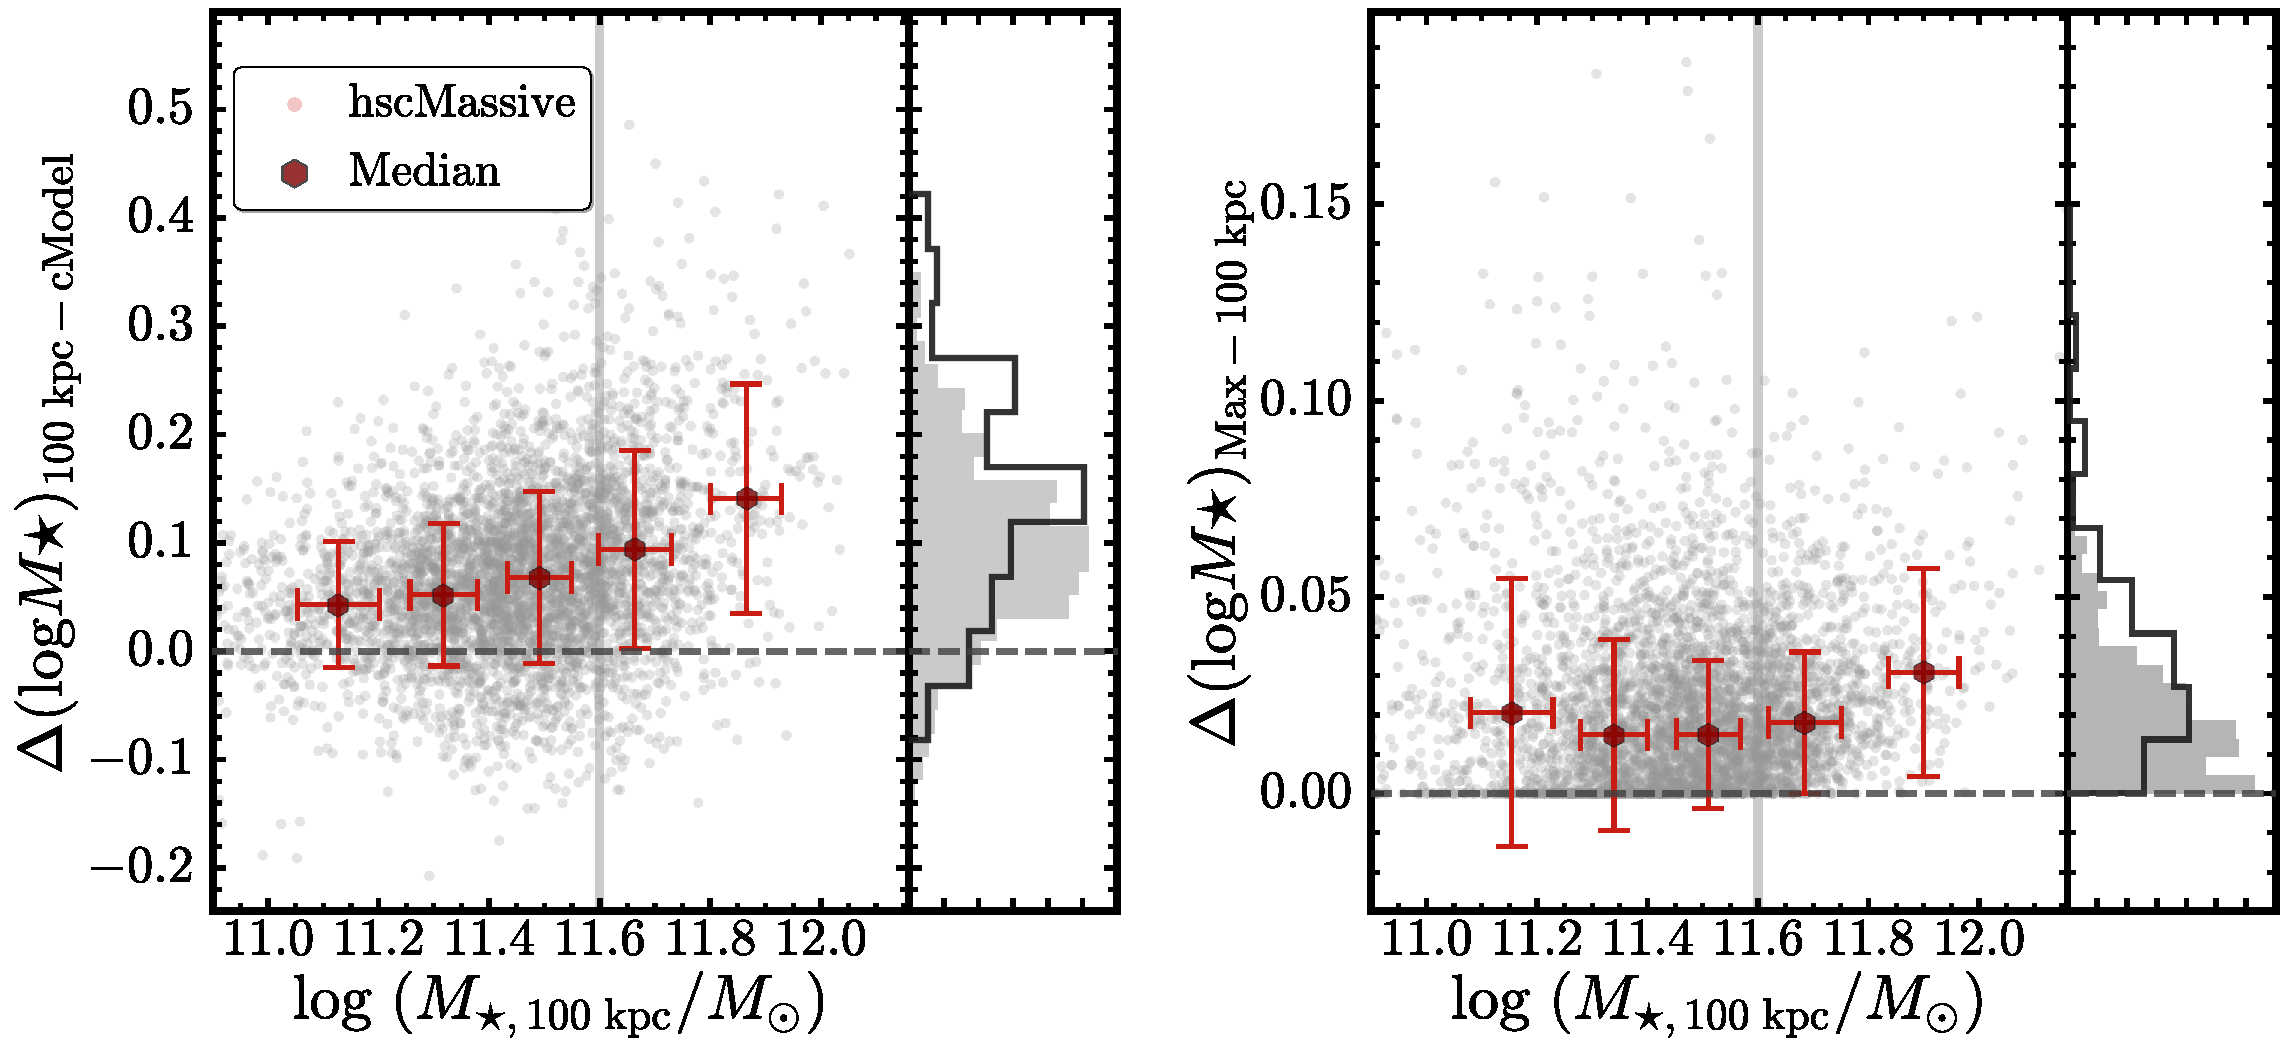
\includegraphics[width=\textwidth]{fig/redbcg_mass_diff_new}
      \caption{              
          \textbf{Left:} Difference between \mcmodel{} and \mtot{} for massive
      	  galaxies (grey dots).
      	  The running-median of the mass differences along with the standard deviations
      	  in a series of mass bins are shown in large red, hexagons with error bars. 
          On average, \mcmodel{} underestimates the total stellar mass of massive 
          galaxies by 0.1 dex while in some cases, the difference can exceed 0.2 dex.
          Vertical histograms indicate the mass difference for all galaxies (shaded 
          histogram) and for the ones with \logmtot{}$>11.6$ (empty histogram).
          \textbf{Right:} Difference between \mmax{} and \mtot{} in the same format. 
          The average difference is small (0.02 dex) and does not show 
          clear mass--dependence. 
          }
      \label{fig:mass_diff}
  \end{figure*}
          
%% ------------------------------------------------------------------------------------ %%
    
%% ------------------------------------------------------------------------------------ %% 
\subsection{Initial Massive Galaxy Sample}
    \label{ssec:initial}
    
    We begin by using a broad luminosity cut to select an initial sample of massive 
    galaxies at $z < 0.5$ from the HSC photometric catalog. 
    Based on \citet{Leauthaud2016}, $i_{\mathrm{SDSS, cModel}} \leq 21.0$ mag can 
    define a sample that includes almost all \logms{}$\geq 11.5$ galaxies.    
    We therefore made a conservative selection of initial sample of massive galaxies
    with $i_{\mathrm{HSC, cModel}} \leq 21.5$\footnote{We neglect small differences
    between the response curves of SDSS-$i$ and HSC-$i$ filters.}
    and also limit our sample to regions that have reached the required depth of 
    the \texttt{WIDE} survey in the $i$-band.
    %% The SQL search is saved as "sample.sql" 
    %% The master catalog used here is "dr1_wide_galaxy_icmodel_21.5.fits"
    %%   The original catalogs contain 2275477 objects
    
    We further select extended objects with no deblending errors, with well defined 
    centroids, and with useful \texttt{cModel} magnitudes in all five bands. 
    After removing objects that have pixels affected by saturation, cosmic-rays, or 
    other optical artifacts\footnote{each criterion removes less than 8\% of the 
    entire sample.}. This sample corresponds to 1760845 galaxies and will be referred 
    as \texttt{hscPho}. 
    %% Saved as "dr1_wide_galaxy_hscPho.fits"      
        
    Here we limit our study to the very high-mass end where the majority of galaxies 
    have either a spectroscopic redshift or a robust red-sequence photo-$z$ from the 
    \redm{} galaxy cluster catalog\footnote{See: http://risa.stanford.edu/redmapper/} 
    (e.g.\ \citealt{Rykoff2014}; \citealt{Rozo2015b}).  
    We match the \texttt{hscPho} sample with a spec-$z$ catalog compiled by the HSC 
    team\footnote{It is created by matching HSC objects with all publicly available 
    spectroscopic redshifts (e.g.\ SDSS/BOSS; GAMA). 
    The spec-$z$ quality flag from different catalogs are homogenized into a single 
    flag that indicates secure redshifts.}.  
    To ensure reasonable \mstar{}-completeness at the high-\mstar{} end we focus on
    the redshift range $0.3 \leq z \leq 0.5$. 
    %% This is catalog: "dr1_specz_use.fits"   
   
    Objects without a spectroscopic redshift are matched with the central 
    galaxies from the \redm{} catalog using a $2.0^{\arcsec}$ matching radius. 
    We keep the matched objects with useful red-sequence photo-$z$ 
    ($0.3 \leq z_{\lambda} < 0.5$) in the final sample. 
    These galaxies are the best candidates for centrals in clusters selected from 
    SDSS DR8 data (\citealt{SDSSDR8}) via a well-tested red-sequence method. 
    The accuracy of the red-sequence photo-$z$ is sufficient (median 
    $|z_{\lambda} - z_{\mathrm{Spec}}| {\sim} 0.01$ for the ones with spec-$z$) 
    for the goal of this work.
    The \redm{} catalog provides an additional 133 unique redshifts for massive 
    galaxies in our sample.
    %% Estimated from "dr1_redbcg_hsc_sdss_gama_1arcsec.fits"
        
    In the end, at $0.3 \leq z \leq 0.5$, we gather a sample of 25286 galaxies with 
    reliable redshift information (referred as \texttt{hscZ}).
    %% Saved as "dr1_wide_galaxy_icmodel_21.5.fits"
    Among them, the BOSS and SDSS ``legacy'' LRG samples provide the majority of 
    spec-$z$. and the GAMA survey provides additional $14$\% of spec-$z$.
    We choose the redshift range of $0.3 \leq z \leq 0.5$ to make sure that 
    (1) The inner region of massive galaxies can be resolved, and \mstar{} within 
    10 kpc can be reliably measured; 
    (2) The background noise and cosmological dimming are not major issues and the 
    \mden{} profile can be measured out to $>100$ kpc; 
    (3) Evolution in structure and stellar population properties can be largely 
    ignored.  
    At both lower and higher redshift, the completeness of spec-$z$ sample starts 
    to decline.  
    Also for bright galaxies at lower redshift, the over-subtraction of background 
    becomes a more serious issue. 
    Before we can define our mass-complete sample of massive galaxies required for 
    our analysis, we describe our one-dimensional photometric analysis 
    (\S \ref{sec:ellipse}) and stellar mass estimations (\S \ref{sec:mstar}). 
    We then define the final sample in \S \ref{sec:final}.
    
%    By comparing with the Stripe 82 Massive Galaxy Catalog
%    (\texttt{S82-MGC}; \citealt{Bundy2015}), \citet{Leauthaud2016} have measured the
%    \mstar{} completeness of the combined BOSS and SDSS samples. 
%    They estimate that the BOSS spec-$z$ sample is about 80\% complete at 
%    \logms{}$\geq 11.6$ at $0.3 < z < 0.5$. 
%    The GAMA survey, which partially overlaps with the HSC footprints, supplements 
%    our \texttt{hscZ} sample by 14\%. 
%    Based on \citet{Taylor2011} (e.g.\ their Fig~~6), at $z{\sim} 0.3$, the GAMA 
%    sample is 80\% complete down to $10^{10.8}$\msun; but only 80\% complete to 
%    $10^{12.0}$\msun at $z{\sim} 0.5$. 
%    We can therefore expect our sample to be roughly \mstar{}-complete above 
%    \logms{}$\geq 11.5$-$11.6$. 
%    This question will be addressed more carefully using the overlap region between 
%    HSC and the \texttt{S82-MGC} in Section \ref{ssec:s82}.

%% ------------------------------------------------------------------------------------ %%  
%\subsection{The \redm{}{} cluster catalog}
%    \label{ssec:redmapper}
%    
%    For now, we wish to focus on galaxies located at the center of their dark matter halos. 
%    To limit our sample to central galaxies, we use \texttt{v5.10} of the \redm{}{} 
%    cluster catalog\footnote{See: http://risa.stanford.edu/redmapper/} 
%    (e.g.\ \citealt{Rykoff2014}; \citealt{Rozo2015b}). 
%    These authors have developed a well-tested red-sequence cluster finder that has 
%    been run on SDSS DR8 (\citealt{SDSSDR8}) photometric data. 
%    For each cluster, the catalog provides a photometric redshift ($z_{\lambda}$), a 
%    cluster richness ($\lambda$), and identifies the most likely central galaxy (the 
%    galaxy with the highest $P_{\mathrm{Cen}}$ value). 
%    The \redm{}{} catalog also provides a list of member galaxies for each cluster and 
%    their associated membership probabilities. 
%    Details about the performance of the \redm{}~cluster catalog can be found in 
%    \citet{Rozo2014}, \citet{Rozo2015a}, and \citet{Rozo2015b}. 
%    Several studies have published calibrations between the \redm{}~richness estimate, 
%    $\lambda$, and halo mass (e.g.\ \citealt{Saro2015, Farahi2016, Simet2016, 
%    Melchior2016}). 
%    All these studies consistently find that \redm{} clusters with $\lambda > 20$ 
%    have $\log (M_{\mathrm{halo}}/M_{\odot}) \geq 14.0$. 
%    The \redm{} catalog therefore helps us group massive central galaxies into 
%    samples with different average \mhalo{}. 
%    We will use the central galaxies of \redm{} clusters 
%    ($P_{\mathrm{CEN}} \geq 0.7$) to form a sample of massive central galaxies that 
%    live in massive halos.
%% ------------------------------------------------------------------------------------ %% 
 
%% ------------------------------------------------------------------------------------ %% 
%\subsection{Massive Central Galaxies in Low and High Mass Halos}
%    \label{ssec:mass_central}
%
%    One of the goals of our work is to investigate the halo dependence of the outer 
%    envelope. Although there is a correlation between $M_{\star}$ and $M_{\mathrm{Halo}}$,
%    based on recent constraints of $M_{\star}$-$M_{\mathrm{Halo}}$ relation 
%    (e.g.\ \citealt{Leauthaud2012}, \citealt{Behroozi2013}, \citealt{Kravtsov2014}), 
%    even though our sample selects very massive galaxies (\logms{}$\geq 11.5$), they 
%    With the help of the \redm{} catalog, we can broadly separate our sample into two
%    groups with \logmh{}$<14.0$ and \logmh{}$>14.2$.
%    live in a fairly broad range of halos masses.
%    
%    % We match this sample with the central galaxies of \redm{}~catalogs using a 
%    % $1.0^{\arcsec}$ radius, and it results in 704 galaxies.  
%    %% Saved as "dr1_redbcg_hsc_sdss_gama_1arcsec.fits"
%    
%    We match the \texttt{hscZ} sample with the central galaxies of \redm{} clusters 
%    with $\lambda \geq 30$ and $P_{\mathrm{0.7}} \geq 0.7$, and find 164 matched 
%    galaxies at $0.3 \leq z \leq 0.5$.
%    Our sample of \textbf{central galaxies in more massive halos} will be referred to 
%    as the \rbcg{} sample. 
%    The median $\lambda$ of the clusters associated with the \rbcg{} sample is 
%    ${\sim} 41$, corresponding to halo mass of 
%    $M_{\mathrm{halo}}{\sim} 2.2\times 10^{14}$ $h^{-1}$ $M_{\odot}$.
%    Only 44 centrals from the \rbcg{} sample live in clusters with $\lambda \geq 50$
%    ($M_{\mathrm{halo}} {\sim} 3.0\times 10^{14}$ $h^{-1} M_{\odot}$). 
%    Our \rbcg{} sample therefore corresponds to galaxies in moderate mass halos.
%    %% Saved as "dr1_redbcg_use_sed5b.fits"
%    
%    Out next goal is to construct a sample of central galaxies living in halos with 
%    \logmh{}$<14.0$. 
%    We first identify and remove all galaxies within a cylindrical region around all 
%    \redm{} clusters. 
%    We use a radius equal to $R_{\mathrm{200b}}$ and the thickness of the cylinder is 
%    set to twice the uncertainty of the photometric redshift error. 
%    We convert $\lambda$ to $M_{\mathrm{halo}}$ using the calibration of 
%    \citet{Simet2016} and we use the mass-concentration relation from 
%    \citet{Diemer2015} to compute $R_{\mathrm{200b}}$. At $0.3 < z < 0.5$, the 
%    uncertainty of photo-$z$ is between 0.015 to 0.025, and is enough to exclude 
%    cluster members.
%    After removing galaxies associated with \redm{} clusters, the remaining galaxies 
%    in our sample will be dominated by central galaxies living in halos with 
%    \logmh{}$\leq 14.0$. 
%    We will refer to this sample of \textbf{central galaxies in less massive halos}
%    as the \nbcg{} sample.
%   
%    Due to the depth and resolution of SDSS, the \redm{} catalog becomes slightly 
%    incomplete at lower richness ($\lambda < 40$) at $z > 0.33$. 
%    To ensure a clean separation in \mhalo{}, here we only focus on the central 
%    galaxies of clusters with $\lambda > 30$. 
%    According to \citet{Simet2016}, this $\lambda \geq 30$ sample should correspond to 
%    $M_{\mathrm{halo}}>10^{14.2} M_{\odot}$. 
%    We have checked that none of the results in this work depend on the choice of this 
%    $\lambda$ limit. 
%    For massive central galaxies that are not in these cluster-level halos, 
%    we unfortunately can not estimate their \mhalo{} individually, but it is safe 
%    to assume they will have $\log (M_{\mathrm{halo}}/M_{\odot}) < 14.0$.  
%    {\bf I am still a bit confused why stellar mass completeness depends on Mh??}
%
%    We note that at this stage, our \nbcg{} sample still contains galaxies with a 
%    wide range of \mstar{} values. 
%    Later on, once we have more accurate \mstar{} estimates, we will further limit this 
%    sample to \logms{}$ > 11.5$. 
%    At this very high mass end, and given that we have rejected satellites in \redm{} 
%    clusters, any further satellite contamination can be safely neglected 
%    (e.g. \citealt{Reid2014, Hoshino2015, Saito2016, vanUitert2016}).
%    %% Saved as "dr1_nonbcg_use_sed5b.fits"
%    
% 
%%% ------------------------------------------------------------------------------------ %% 

%% ------------------------------------------------------------------------------------ %% 
%\subsection{Summary of Sample Construction}
%    \label{ssec:sample}
%
%    Using ${\sim} 100$ deg$^2$ of HSC data, we select a large sample of massive central 
%    galaxies with reliable redshift information, and broadly separate them two 
%    categories based on $M_{\mathrm{halo}}$.
%    
%    The following is a summary of our sample construction.
%    
%    \begin{itemize}
%        \item \texttt{hscPho} sample: this parent sample consists of bright galaxies 
%            with $i_{\mathrm{cModel}} \leq 21.0$, good quality imaging, and reliable 
%            \texttt{cModel} photometry in all five HSC bands in the \texttt{S15B} 
%            data release. 
%        \item \texttt{hscZ} sample: we limit the \texttt{hscPho} sample to galaxies 
%            with reliable redshift information. 
%        \item {\bf Select only central galaxies using RedMapper: total number in full 
%        sample?}
%        \item We further divide the sample into an \rbcg{} sample and a \nbcg{} sample, 
%          with the former roughly having \logmh{}$\geq 14.2$ and the latter having 
%           \logmh{}$<14.0$.
%
%          : we select a sample of 164 galaxies at 
%            $0.3 \leq z \leq 0.5$ that are the central galaxies 
%            in $\lambda > 30$ \redm{} clusters. 
%            They represent the central galaxies in very massive halos 
%            (\logmh{}$\geq 14.2$). 
%        \item \nbcg{} sample: after excluding all cluster members from the 
%            \texttt{hscZ} sample, we have 14661 bright galaxies at 
%            $0.3 \leq z \leq 0.5$. 
%            After applying an additional \mstar{} cut (see Section 
%            \ref{ssec:isedfit}), this sample corresponds to central galaxies in 
%            halos with \logmh{}$<14.0$.  
%    \end{itemize}
%    
%    We now proceed to measure the luminosities and stellar mass profiles for 
%    all galaxies in the \rbcg{} and \nbcg{} samples.
%% ------------------------------------------------------------------------------------ %% 

%% ------------------------------------------------------------------------------------ %% 
\section{Measurements of 1-D Surface Brightness Profiles}
    \label{sec:ellipse}
    
    The surface brightness profile of massive ETG can not be well modeled by the 
    de~Vaucouleurs or single-\ser law, especially at the imaging depth of HSC.
    These models will fail to simultaneously describe the profile in both the inner 
    and the outer regions and also cannot account for any radial variations in 
    ellipticity and position angle. 
    In principle, massive galaxies can still be described by more complex 
    models (e.g \citealt{Huang2013a, Huang2013b, Oh2017}), but they are still 
    sensitive to the choices of models (e.g. de~Vaucouleurs or \ser{} profile), 
    the number of components, initial guesses of parameters, and the internal 
    degeneracies among different parameters. 
    Background subtraction uncertainty also affects the 2-D model fitting 
    dramatically, especially for massive ETGs in our sample. 
    We therefore perform elliptical isophote fitting using the IRAF \texttt{Ellipse} 
    algorithm (Jedrzejewski 1987) to estimate the total luminosities of massive 
    galaxies and measure their one-dimensional profiles of stellar mass surface 
    density (\mden{}). 
    This 1-D method we adopt is less affected by the issues mentioned above. 
    Also, we will only study galaxies in the radial range where we are not 
    sensitive to either the PSF ($r<3-5$ kpc) or the background subtraction 
    ($r>100$ kpc). 
        
    We prepare large $i$-band cut-outs for each galaxy that extend to 750 kpc in 
    radius, along with a bad pixel mask and the PSF model. 
    These cut-outs include all of the light of the galaxy and are large enough to 
    also evaluate the background level. 
    We choose to use $i$-band images because they trace the stellar distributions of 
    massive galaxies at $0.3 \leq z \leq 0.5$ reasonably well 
    (the observed i-band corresponds to a rest-frame $g$ or $r$ band), but also 
    because they have better seeing and much lower background levels than the $z$ 
    and $y$ band images (although these in principle may be better tracers of 
    \mden{}). 
    
    For each cut-out, to overcome the \texttt{hscPipe} ``over-deblending'' issue, 
    we use a customized procedure to detect and aggressively mask out
    neighbouring objects. 
    Furthermore, \texttt{hscPipe} tends to over-subtract the background around 
    bright objects. 
    To improve the background subtraction, we first aggressively mask 
    out all objects (including the central massive galaxy), and derive an 
    empirical background correction using \texttt{SExtractor}.
    Then, we run \texttt{Ellipse} on the background-corrected, masked cut-outs 
    following the methodology of \citet{Li2012}. 
    In short, we first fit each isophote using a free centroid and shape 
    (ellipticity and position angle). 
    We then fix the centroid (using the mean flux-weighted centroid) and estimate
    the mean ellipticity and position angles of all isophotes. 
    Finally, we extract a 1-D surface brightness profile along the major axis using 
    the mean ellipticity and position angle. 
    We correct these surface brightness profiles for Galactic extinction and 
    cosmological dimming, and integrate them to various radii to get the luminosity 
    within different physical (elliptical) apertures. 
    Fig~\ref{fig:ellipse} shows an example of the 1-D surface brightness and 
    ellipticity profile for a massive galaxy at $z{\sim}0.2$ and also highlights 
    a few isophotes.    

    We test our procedure using different mask sizes, different \texttt{Ellipse} 
    parameters, and with or without our background correction. 
    Based on these tests, we find that our 1-D surface brightness profiles are reliable 
    up to surfaces brightness levels of $i{\sim}28.5$ \sb. 
    Beyond that, some of our profiles shows signs of truncation and/or large 
    fluctuations which are due to either the uncertainty in the background 
    subtraction or the unmasked flux from other objects.
    We choose to limit our study to surface brightness levels up to ${\sim} 28.5$ \sb. 
    This is a conservative choice but already enables us to measure light profiles 
    out to $100$ kpc on a galaxy-by-galaxy basis (no stacking). 
    For more technical details of the \texttt{Ellipse} procedure, please see 
    Appendix~\ref{app:ellipse}.

%% ------------------------------------------------------------------------------------ %% 
    
    For physical (e.g.\ late-stage major merger) and nuisance (e.g.\ nearby foreground 
    galaxy or bright star) reasons, we cannot extract reliable 1-D profiles for a small 
    fraction of massive galaxies because they are heavily masked out. 
    This is an intrinsic limitation of the 1-D method, and it removes ${\sim}10$\% of 
    the sample.
    %It affects $18/164$ of the \rbcg{} sample, and a smaller fraction of the 
    %\nbcg{} sample. 
    It is worth noting that this excludes most major-merging massive galaxies. 
    
    Given our exquisite profiles that extend to 100 kpc, the definition and meaning 
    of ``total'' magnitude (and stellar mass) becomes more nuanced.
    With the help of the \m2l{} estimated in the next section (\S \ref{sec:mstar}), 
    we integrate the profile to a range of radii, and estimate the stellar mass 
    within these different apertures.  
    Motivated by the two-phase scenario, we will consider two benchmark physical 
    apertures throughout this work:
    
    \begin{itemize} 
       
        \item \textbf{The \mstar{} within the inner 10 kpc} 
            (hereafter noted \minn{}). 
            According to the two-phase scenario, the ``in-situ'' star-formation 
            quickly builds up the inner, dense core of massive ETGs.  
            Based on recent observation (e.g.~\citealt{vanDokkum2010}) and 
            simulations (e.g. \citealt{RodriguezGomez2016}), the in-situ component
            dominates the \mstar{} within one effective radius ($R_{\mathrm{e}}$, 
            or 5-10 kpc) of $z{\sim}0$ massive ETGs.
            We therefore use \minn{} as proxy for the mass forged during the 
            ``in-situ'' phase. 
            Given the quality of the HSC data, we can reliably measure \minn{} over 
            our redshift range ($1.0^{\arcsec}$ in radius equals 4.4 and 6.1 kpc 
            at redshift 0.3 and 0.5).  
            It is worth noting that, at very high-\mstar{} end, there can be 
            significant contribution of accreted stars within 10 kpc 
            (e.g. \citealt{RodriguezGomez2016}). 
            We will further discuss the justification of this assumption in 
            \ref{ssec:twophase}.
            
        \item \textbf{The stellar mass within 100 kpc} 
            (hereafter noted \mtot{}). 
            For our galaxy sample, a 100 kpc aperture corresponds to 5-10 
            $\times R_{\mathrm{e}}$. 
            We show in section \ref{ssec:mtotal} that most of the \mstar{} for 
            these ETGs can be captured by a 100 kpc radius and that \mtot{} is 
            a good proxy for the ``total'' \mstar{}. 
            Although not perfect, we argue that our measurements of \mtot{} (which are 
            actually measuring the light directly out to 100 kpc) are a better tracer 
            of total \mstar{} than model-dependent results from shallower data 
            (such as SDSS) which rely on extrapolating the light profiles of galaxies 
            out to large radii.
            
       \end{itemize}
       
%% ------------------------------------------------------------------------------------ %% 
    
%% ------------------------------------------------------------------------------------ %% 
\section{Stellar Masses and Mass Density Profiles}
    \label{sec:mstar}
    
%% ------------------------------------------------------------------------------------ %% 
\subsection{Stellar Masses from SED Fitting}
    \label{ssec:isedfit}
   
    To convert luminosities into \mstar{}, we assume that these massive galaxies 
    can be well described by an average \m2l{}. 
    This is a reasonable assumption considering that they are mostly dominated by 
    old stellar populations and are known to have only shallow color gradients. 
    We will further justify this point by measuring their median color profiles in 
    Section \ref{ssec:ell_color}.

    We use the broadband Spectral Energy Distributions (SEDs) fitting 
    (see \citealt{Walcher2011} for a recent review) code 
    \texttt{iSEDFit}\footnote{http://www.sos.siena.edu/~jmoustakas/isedfit/} 
    (\citealt{Moustakas13}) to estimate the average \m2l{} and $k$-corrections using
    5-band HSC \cmodel{} fluxes.
    Although \cmodel{} tends to underestimate the total flux for bright, extended 
    objects, it can still yield accurate \emph{average} colors thanks to the 
    forced-photometry method that takes the PSF convolution into account
    (e.g. \citealt{SynPipe}). 

    \texttt{iSEDFit} takes a simplified Bayesian approach. 
    In short, it first generates a large grid of SEDs from synthetic stellar 
    population models by drawing randomly from the prior distributions of relevant
    parameters (e.g. age, metallicity, dust extinction, and star formation history).
    Based on these models, it uses the observed photometry and redshift to compute 
    the statistical likelihood, and generates the posterior probability distribution 
    functions (PDF) for each parameter.  
    To get the best estimate of a given parameter, \texttt{iSEDFit} integrates the 
    full PDF over all the other nuisance parameters.
    Then, the median value and the 1-$\sigma$ uncertainty are derived based on the 
    marginalized PDF. 
    Please refer to \citet{Moustakas13} for technical details. 
    
    In this work, we derive average \m2l{} using the Flexible Stellar Population 
    Synthesis\footnote{http://scholar.harvard.edu/cconroy/sps-models}
    (FSPS; \texttt{v2.4}; \citealt{FSPS}, \citealt{Conroy2010}) model based on the 
    MILES\footnote{http://www.iac.es/proyecto/miles/pages/stellar-libraries}
    (\citealt{MILES1}, \citealt{MILES2}) stellar library and assuming a
    \citet{Chabrier2003} IMF between 0.1 to 100 \msun. 
    The star formation history (SFH) is assumed to follow a delayed-$\tau$ model with 
    stochastic star bursts (see Appendix~\ref{app:sed}). 
    This SFH is appropriate for massive galaxies at low redshifts 
    (e.g.\ \citealt{Kauffmann2003}). 
    For stellar metallicity 
    ($[\mathrm{M}/\mathrm{H}]=\log\ \mathrm{Z}/\mathrm{Z}_{\odot}$), we assume a flat 
    distribution between 0.004 to 0.03 (the highest value allowed by FSPS).
    We adopt the \citet{Calzetti2000} extinction law with a order two Gamma 
    distribution of $A_{V}$ between 0 to 2 magnitude. 
    The majority of our galaxies are red and quiescent ones so the results are not 
    very sensitive to parameters related to the SFH or the internal dust extinction. 
    To achieve reasonable sampling across these parameters, we generate 250000 models. 
    
    We construct five band SEDs using the forced-photometry \cmodel{} magnitudes 
    corrected for Galactic extinction. 
    \cmodel{} only accounts for the statistical error on the flux measurement but 
    does not account for systematic uncertainties in the model-fitting process. 
    It therefore underestimates the flux errors of bright galaxies. 
    For this work, we supply \texttt{iSEDFit} with simplified flux errors assuming 
    $S/N = 100$ for the $riz$ bands, and $S/N = 80$ for the $g$ and $y$ band 
    (on average, images in $gy$ bands are shallower in depth and/or have higher 
    background noise).  
    Although these are still conservative estimates of the systematic uncertainties 
    involved in the model-fitting, tests using synthetic galaxies show that \cmodel{}
    provides excellent measurements of five-band colors, which are crucial for 
    reliable \m2l{} estimates.
    The typical uncertainty of \logms{} is around 0.06-0.08 dex at \logms${\sim} 11.5$. 
    Please see Appendix~\ref{app:sed} for further details.
      
%% ------------------------------------------------------------------------------------ %%  

%% ------------------------------------------------------------------------------------ %% 
\subsection{``Total'' Stellar Masses}
    \label{ssec:mtotal}
    
    Using the best-fit stellar mass from \texttt{iSEDFit} (noted as as \mcmodel{}), 
    we estimate the average \m2l{} in the $i$-band, then use that \m2l{} to convert 
    our 1-D luminosity density profiles into stellar mass density (\mden{}) profiles. 
    We also convert our 10 and 100 kpc aperture luminosities into corresponding stellar 
    mass estimates (noted as \minn{} and \mtot{}).
    
    For the remainder of this paper, we will use \mtot{} as a proxy of ``total'' 
    stellar mass. 
    \update{
    As expected, the integration of the 1-D profile out to very large radius recovers 
    more luminosity (stellar mass) compared to the \cmodel{}-based estimates 
    (Fig \ref{fig:mass_diff}).
    }
    \song{Work in progress.}
    
    In Appendix~\ref{app:sed}, we briefly summarize the basic statistics of 
    the sample using our estimates of \mtot{} and \minn{}.
    We confirm that the sample follows a very tight ``red-sequence'' that does not appear to depend on 
    environment (see \S XX). 
    Appendix~\ref{app:sed} describes the outputs from our SED fitting process 
    (average stellar age, metallicity, and internal dust extinction). 
    We do not utilize these quantities in this paper, but we have checked that they all 
    behave reasonably for both samples. 

    \song{The color gradients and ellipticity profiles will be updated}
    Our methodology ignores any radial variations in \m2l{}. 
    It is well known that massive ETGs have negative optical color gradients indicating 
    gradients in \m2l{} (e.g.\ \citealt{LaBarbera2012}; 
    \citealt{DSouza2015}). \jenny{earlier reference here?}
    These color gradients are shallow and smooth out to a few times the effective 
    radius and color gradients at the outskirts are not yet well quantified.
    Our results looking at the outer envelopes as a function of mass and environment 
    will be robust as long as there is \emph{no significant difference in 
    the average color gradient between sub-samples}.
    %More importantly, for the comparison between the \rbcg{} and \nbcg{} samples, 
    %our results will be robust as long as there is \emph{no significant difference in 
    %the average color gradient between the two samples}. 
    We have confirmed that this is indeed the case (see Section~\ref{ssec:ell_color}). 
    
    Our method for deriving total stellar masses is similar to the 
    method adopted by the GAMA survey (\citealt{Taylor2011, Kelvin2012}). 
    We have compared our \mstar{} values with those from GAMA and the results are given 
    in Appendix~\ref{app:gama}. 
    We find a systematic differences between the two \mstar{} estimates.
    It is likely that the GAMA models fail to capture the flux associated with the 
    outskirts of galaxies due to the limited depth of SDSS.     
%% ------------------------------------------------------------------------------------ %% 

%% ------------------------------------------------------------------------------------ %%        
    \subsection{Stellar Mass Completeness}
    \label{ssec:complete}
    
    With the help of the \texttt{S82-MGC} (\citealt{Bundy2015}), we investigate the 
    \mstar{} completeness of our samples. 
    The \texttt{S82-MGC} sample matches the deeper SDSS photometric data in the 
    Stripe 82 region (\citealt{Annis2014}) with the near infrared data from the United 
    Kingdom Infrared Telescope Infrared Deep Sky Survey (UKIDSS; \citealt{Lawrence2007}). 
    The deeper photometry and better photo-$z$s make the \texttt{S82-MGC} sample complete 
    to \logms{}$\geq 11.2$ at $z<0.7$ which makes it sufficient to evaluate the 
    completeness of our HSC samples.
    
    There are 20453 \texttt{S82-MGC} galaxies that are also in the \texttt{hscPho} 
    sample at $0.3 \leq z_{\mathrm{s82}} \leq 0.5$. 
    We compute \mstar{} values for these galaxies using our fiducial 
    procedure\footnote{The \mstar{} using HSC photometry is in excellent with the 
    values derived from the \texttt{S82-MGC} which includes NIR data from UKIDSS; 
    \texttt{S82-MGC} also uses \texttt{iSEDFit} with similar assumptions.}. 
    Figure~\ref{fig:mass_complete} compares the SMFs of galaxies from 
    \texttt{S82-MGC} with the SMFs of galaxies from our 
    sample\footnote{Errors on the SMFs are estimated via bootstrap resampling}. 
    Based on Fig~\ref{fig:mass_complete}, we conclude that our sample of massive galaxies is 
    reasonably complete down to \logms{}${\sim} 11.6$ at $0.3 \leq z \leq 0.5$. 
    %The \rbcg{} sample is less affected by completeness because we can utilize 
    %photo-$z$s from \redm{}. 
    %However, the completeness of the \nbcg{} sample is still limited by the 
    %availability of spec-$z$s from BOSS.    
    In this work, we will focus on the range $11.6 \le$ \logmtot{}$ \le 11.9$ 
    where our two samples are complete. 
    %When comparing \nbcg{} and \rbcg{} we will also always make sure that the two 
    %samples are well matched both in terms of \mstar{} as well as in terms of redshift. 
    %Please see the next section and Appendix~\ref{app:match} for more details.
    
	\jenny{Anything else we need to keep from here?}
	By comparing with the Stripe 82 Massive Galaxy Catalog
    (\texttt{S82-MGC}; \citealt{Bundy2015}), \citet{Leauthaud2016} have measured the
    \mstar{} completeness of the combined BOSS and SDSS samples. 
    They estimate that the BOSS spec-$z$ sample is about 80\% complete at 
    \logms{}$\geq 11.6$ at $0.3 < z < 0.5$. 
    The GAMA survey, which partially overlaps with the HSC footprints, supplements 
    our \texttt{hscZ} sample by 14\%. 
    Based on \citet{Taylor2011} (e.g.\ their Fig~~6), at $z{\sim} 0.3$, the GAMA 
    sample is 80\% complete down to $10^{10.8}$\msun; but only 80\% complete to 
    $10^{12.0}$\msun at $z{\sim} 0.5$. 
    We can therefore expect our sample to be roughly \mstar{}-complete above 
    \logms{}$\geq 11.5$-$11.6$. 
    This question will be addressed more carefully using the overlap region between 
    HSC and the \texttt{S82-MGC} in Section \ref{ssec:s82}.
%% ------------------------------------------------------------------------------------ %%

%% ------------------------------------------------------------------------------------ %%  
\section{The Final Sample}
    \label{sec:final}
    
	With stellar masses in hand, we now use the redMapper cluster catalog to identify a sample of 
    central galaxies.

	\subsection{Indentifying central galaxies using the \redm{}{} cluster catalog}
    \label{ssec:redmapper}
    
    We wish to focus on galaxies located at the center of their dark matter halos. 
    To limit our sample to central galaxies, we use \texttt{v5.10} of the \redm{}{} 
    cluster catalog\footnote{See: http://risa.stanford.edu/redmapper/} 
    (e.g.\ \citealt{Rykoff2014}; \citealt{Rozo2015b}). 
    These authors have developed a well-tested red-sequence cluster finder that has 
    been run on SDSS DR8 (\citealt{SDSSDR8}) photometric data. 
    For each cluster, the catalog provides a photometric redshift ($z_{\lambda}$), a 
    cluster richness ($\lambda$), and identifies the most likely central galaxy (the 
    galaxy with the highest $P_{\mathrm{Cen}}$ value). 
    The \redm{}{} catalog also provides a list of member galaxies for each cluster and 
    their associated membership probabilities. 
    Details about the performance of the \redm{}~cluster catalog can be found in 
    \citet{Rozo2014}, \citet{Rozo2015a}, and \citet{Rozo2015b}. 
    
    Several studies have published calibrations between the \redm{}~richness estimate, 
    $\lambda$, and halo mass (e.g.\ \citealt{Saro2015, Farahi2016, Simet2016, 
    Melchior2016}). 
    All these studies consistently find that \redm{} clusters with $\lambda > 20$ 
    have $\log (M_{\mathrm{halo}}/M_{\odot}) \geq 14.0$. 
    The \redm{} catalog therefore helps us group massive central galaxies into 
    samples with different average \mhalo{}. 
    We will use the central galaxies of \redm{} clusters 
    ($P_{\mathrm{CEN}} \geq 0.7$) to form a sample of massive central galaxies that 
    live in massive halos as described below. In addition to identifying central galaxies, 
    we are also able to link each galaxy with a halo mass using the redMaPPer catalog, and 
    this information is also very useful in studying the 
    relationship between galaxy structure and environment.
%% ------------------------------------------------------------------------------------ %% 

%% ------------------------------------------------------------------------------------ %% 
  \begin{figure}
      \centering 
      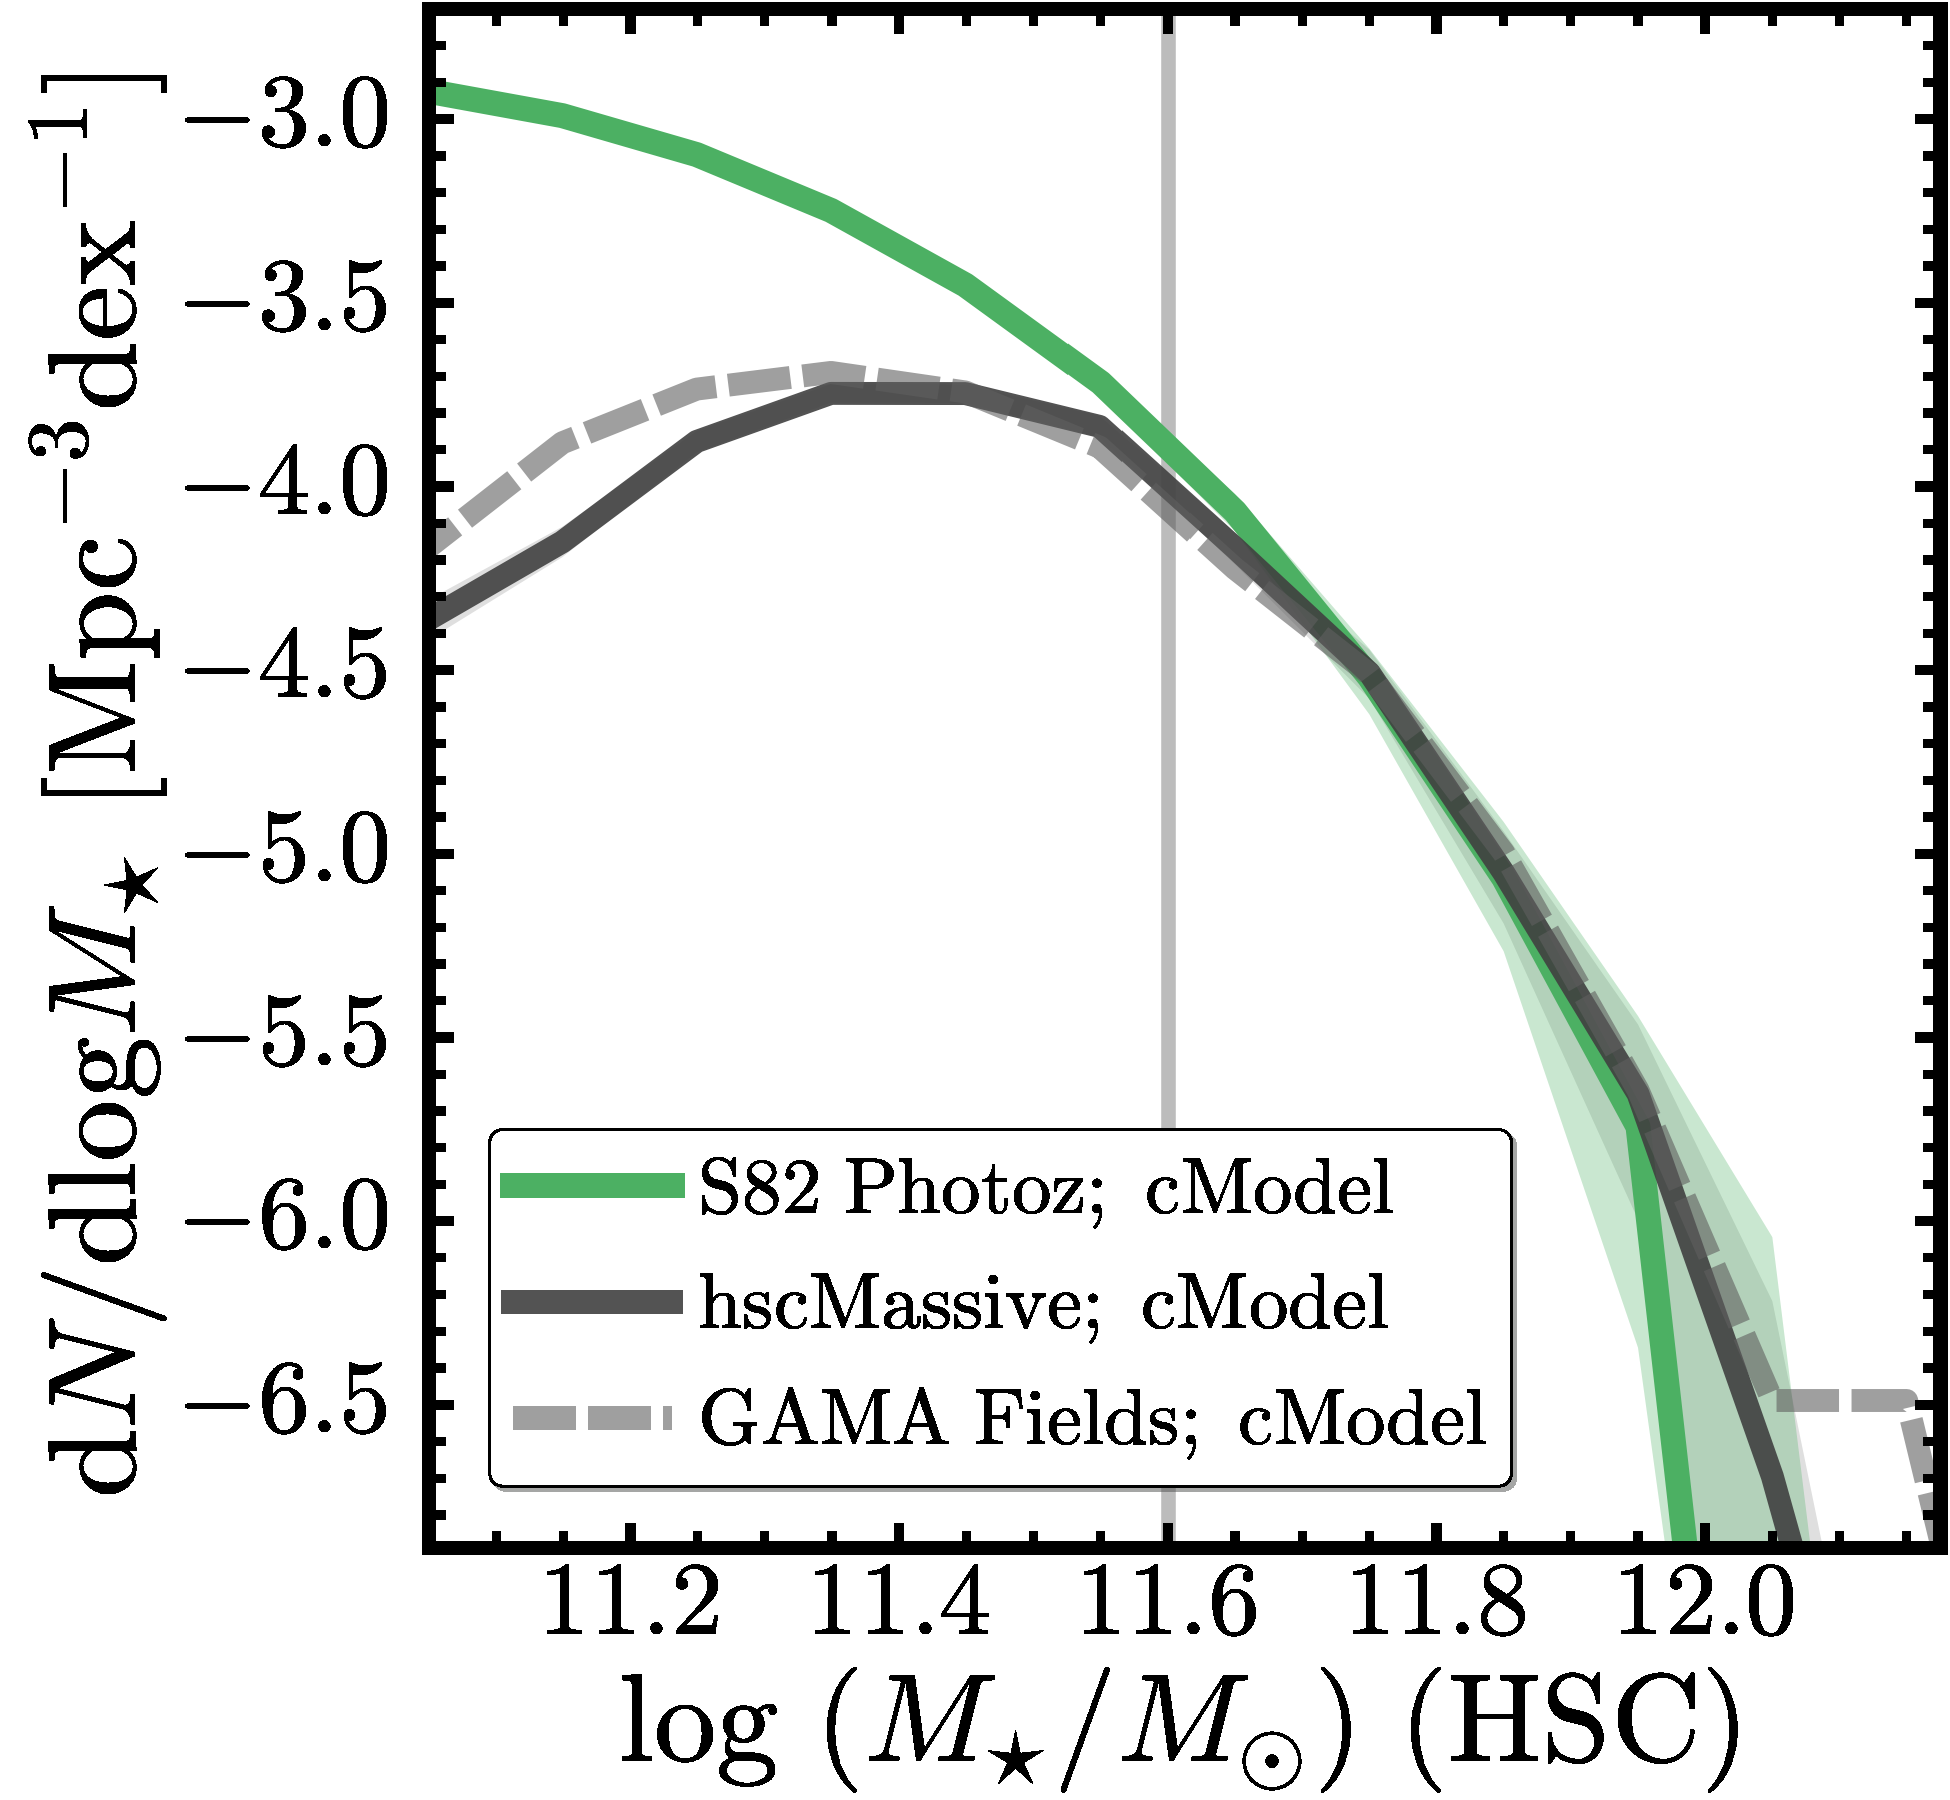
\includegraphics[width=\columnwidth]{fig/redbcg_completeness}
      \caption{
          Evaluation of the \mstar{} completeness of the HSC massive galaxy sample.
          We compare the volume number density function of the massive galaxies 
          for this work (black line) with the one of a much more complete sample
          from the S82-MGC catalog (green line).  
          The associated uncertainties derived from bootstrap resampling are shown in 
          shaded regions. 
          The vertical grey line highlight the \logms{}$=11.6$ limit.  
          Below it, the HSC massive galaxy sample becomes significantly incomplete in 
          stellar mass. 
          }
      \label{fig:mass_complete}
  \end{figure}     
%% ------------------------------------------------------------------------------------ %%
 
%% ------------------------------------------------------------------------------------ %% 
%\subsection{Massive Central Galaxies in Low and High Mass Halos}
%    \label{ssec:mass_central}

    %One of the goals of our work is to investigate the halo dependence of the outer 
    %envelope. Although there is a correlation between $M_{\star}$ and $M_{\mathrm{Halo}}$,
    %based on recent constraints of $M_{\star}$-$M_{\mathrm{Halo}}$ relation 
    %(e.g.\ \citealt{Leauthaud2012}, \citealt{Behroozi2013}, \citealt{Kravtsov2014}), 
    %even though our sample selects very massive galaxies (\logms{}$\geq 11.5$), they 
    %With the help of the \redm{} catalog, we can broadly separate our sample into two
    %groups with \logmh{}$<14.0$ and \logmh{}$>14.2$.
    %live in a fairly broad range of halos masses.
    
    % We match this sample with the central galaxies of \redm{}~catalogs using a 
    % $1.0^{\arcsec}$ radius, and it results in 704 galaxies.  
    %% Saved as "dr1_redbcg_hsc_sdss_gama_1arcsec.fits"
    
    Due to the depth and resolution of SDSS, the \redm{} catalog becomes slightly 
    incomplete at lower richness ($\lambda < 40$) at $z > 0.33$. 
    To ensure a clean separation in \mhalo{}, here we only focus on the central 
    galaxies of clusters with $\lambda > 30$. 
    According to \citet{Simet2016}, this $\lambda \geq 30$ sample should correspond to 
    $M_{\mathrm{halo}}>10^{14.2} M_{\odot}$. 
    We have checked that none of the results in this work depend on the choice of this 
    $\lambda$ limit.
    
    We therefore match the \texttt{hscZ} sample with the central galaxies of \redm{} clusters 
    with $\lambda \geq 30$ and $P_{\mathrm{0.7}} \geq 0.7$, and find 164 matched 
    galaxies at $0.3 \leq z \leq 0.5$.
    Our sample of \textbf{central galaxies in more massive halos} will be referred to 
    as the \rbcg{} sample. 
    The median $\lambda$ of the clusters associated with the \rbcg{} sample is 
    ${\sim} 41$, corresponding to halo mass of 
    $M_{\mathrm{halo}}{\sim} 2.2\times 10^{14}$ $h^{-1}$ $M_{\odot}$.
    Only 44 centrals from the \rbcg{} sample live in clusters with $\lambda \geq 50$
    ($M_{\mathrm{halo}} {\sim} 3.0\times 10^{14}$ $h^{-1} M_{\odot}$). 
    Our \rbcg{} sample therefore corresponds to galaxies in moderate mass halos.
    %% Saved as "dr1_redbcg_use_sed5b.fits"
    
    Out next goal is to construct a sample of central galaxies living in halos with 
    \logmh{}$<14.0$. 
    We first identify and remove all galaxies within a cylindrical region around all 
    \redm{} clusters. 
    We use a radius equal to $R_{\mathrm{200b}}$ and the thickness of the cylinder is 
    set to twice the uncertainty of the photometric redshift error. 
    We convert $\lambda$ to $M_{\mathrm{halo}}$ using the calibration of 
    \citet{Simet2016} and we use the mass-concentration relation from 
    \citet{Diemer2015} to compute $R_{\mathrm{200b}}$. At $0.3 < z < 0.5$, the 
    uncertainty of photo-$z$ is between 0.015 to 0.025, and is enough to exclude 
    cluster members.
    After removing galaxies associated with \redm{} clusters, the remaining galaxies 
    in our sample will be dominated by central galaxies living in halos with 
    \logmh{}$\leq 14.0$. 
    We will refer to this sample of \textbf{central galaxies in less massive halos}
    as the \nbcg{} sample. For massive central galaxies that are not in these cluster-level halos, 
    we unfortunately can not estimate their \mhalo{} individually, but it is safe 
    to assume they will have $\log (M_{\mathrm{halo}}/M_{\odot}) < 14.0$.  
    At this very high mass end, and given that we have rejected satellites in \redm{} 
    clusters, any further satellite contamination can be safely neglected 
    (e.g. \citealt{Reid2014, Hoshino2015, Saito2016, vanUitert2016}).
    %% Saved as "dr1_nonbcg_use_sed5b.fits"
    % TODO: The actual number waits to be updated}
    
 
%% ------------------------------------------------------------------------------------ %% 

%% ------------------------------------------------------------------------------------ %% 
\subsection{Summary of Sample Construction}
    \label{ssec:sample}

    Using ${\sim} 100$ deg$^2$ of HSC data, we select a large sample of massive central 
    galaxies with reliable redshift information, and broadly separate them two 
    categories based on $M_{\mathrm{halo}}$.
    
    The following is a summary of our sample construction.
    
    \begin{itemize}
        \item \texttt{hscPho} sample: this parent sample consists of bright galaxies 
            with $i_{\mathrm{cModel}} \leq 21.0$, good quality imaging, and reliable 
            \texttt{cModel} photometry in all five HSC bands in the \texttt{S15B} 
            data release. 
        \item \texttt{hscZ} sample: we limit the \texttt{hscPho} sample to galaxies 
            with reliable redshift information. 
        \item We further divide the sample into an \rbcg{} sample and a \nbcg{} sample, 
          with the former roughly having \logmh{}$\geq 14.2$ and the latter having 
           \logmh{}$<14.0$.

%          : we select a sample of 164 galaxies at 
%            $0.3 \leq z \leq 0.5$ that are the central galaxies 
%            in $\lambda > 30$ \redm{} clusters. 
%            They represent the central galaxies in very massive halos 
%            (\logmh{}$\geq 14.2$). 
%        \item \nbcg{} sample: after excluding all cluster members from the 
%            \texttt{hscZ} sample, we have 14661 bright galaxies at 
%            $0.3 \leq z \leq 0.5$. 
%            After applying an additional \mstar{} cut (see Section 
%            \ref{ssec:isedfit}), this sample corresponds to central galaxies in 
%            halos with \logmh{}$<14.0$.  
    \end{itemize}
    
%% ------------------------------------------------------------------------------------ %% 


 
%% ------------------------------------------------------------------------------------ %% 
\section{Results}
    \label{sec:result}

%% ------------------------------------------------------------------------------------ %%     
    \subsection{Impact of Missing Light on the Galaxy Stellar Mass Function}
    \label{ssec:s82}
    
    Different methods for estimating the ``total'' \mstar{} can have a large impact on 
    the high mass end of the galaxy stellar mass function (e.g. \citealt{Bernardi2013, 
    DSouza2014, DSouza2015, Bernardi2016a}). 
    Fig~\ref{fig:mass_complete} shows the SMF computed using both \mtot{} and \mcmodel{}. 
    As can be seen from this figure, our careful 1-D approach recovers more flux 
    in massive galaxies than \texttt{cModel}. 
    More importantly, the average difference steadily increases with \mtot{}. 
    At \logms{} $>11.5$, the difference can be larger than 0.2 dex. 
    This difference relates to the intrinsic limitation of the \texttt{cModel} method 
    and also reflects the fact that more massive ETGs tend to have more extended 
    stellar mass distributions (e.g. \citealt{Graham2003}). 
    Generally speaking, the use of \mtot{} instead of the \mcmodel{} shifts the SMF 
    towards the higher-mass end and slightly modifies the high-mass slope. 
    %The impact of missing flux is most prominent for the \rbcg{} sample.
    For studies about the SMF or other aspects of galaxy evolution based on 
    \cmodel{}-like photometry or shallower images, these effects can not be neglected.
%% ------------------------------------------------------------------------------------ %%  

%% ------------------------------------------------------------------------------------ %%
\subsection{Surface Mass Density Profiles}
    \label{ssec:sbp_compare}

%% ------------------------------------------------------------------------------------ %% 
  \begin{figure*}
      \centering 
      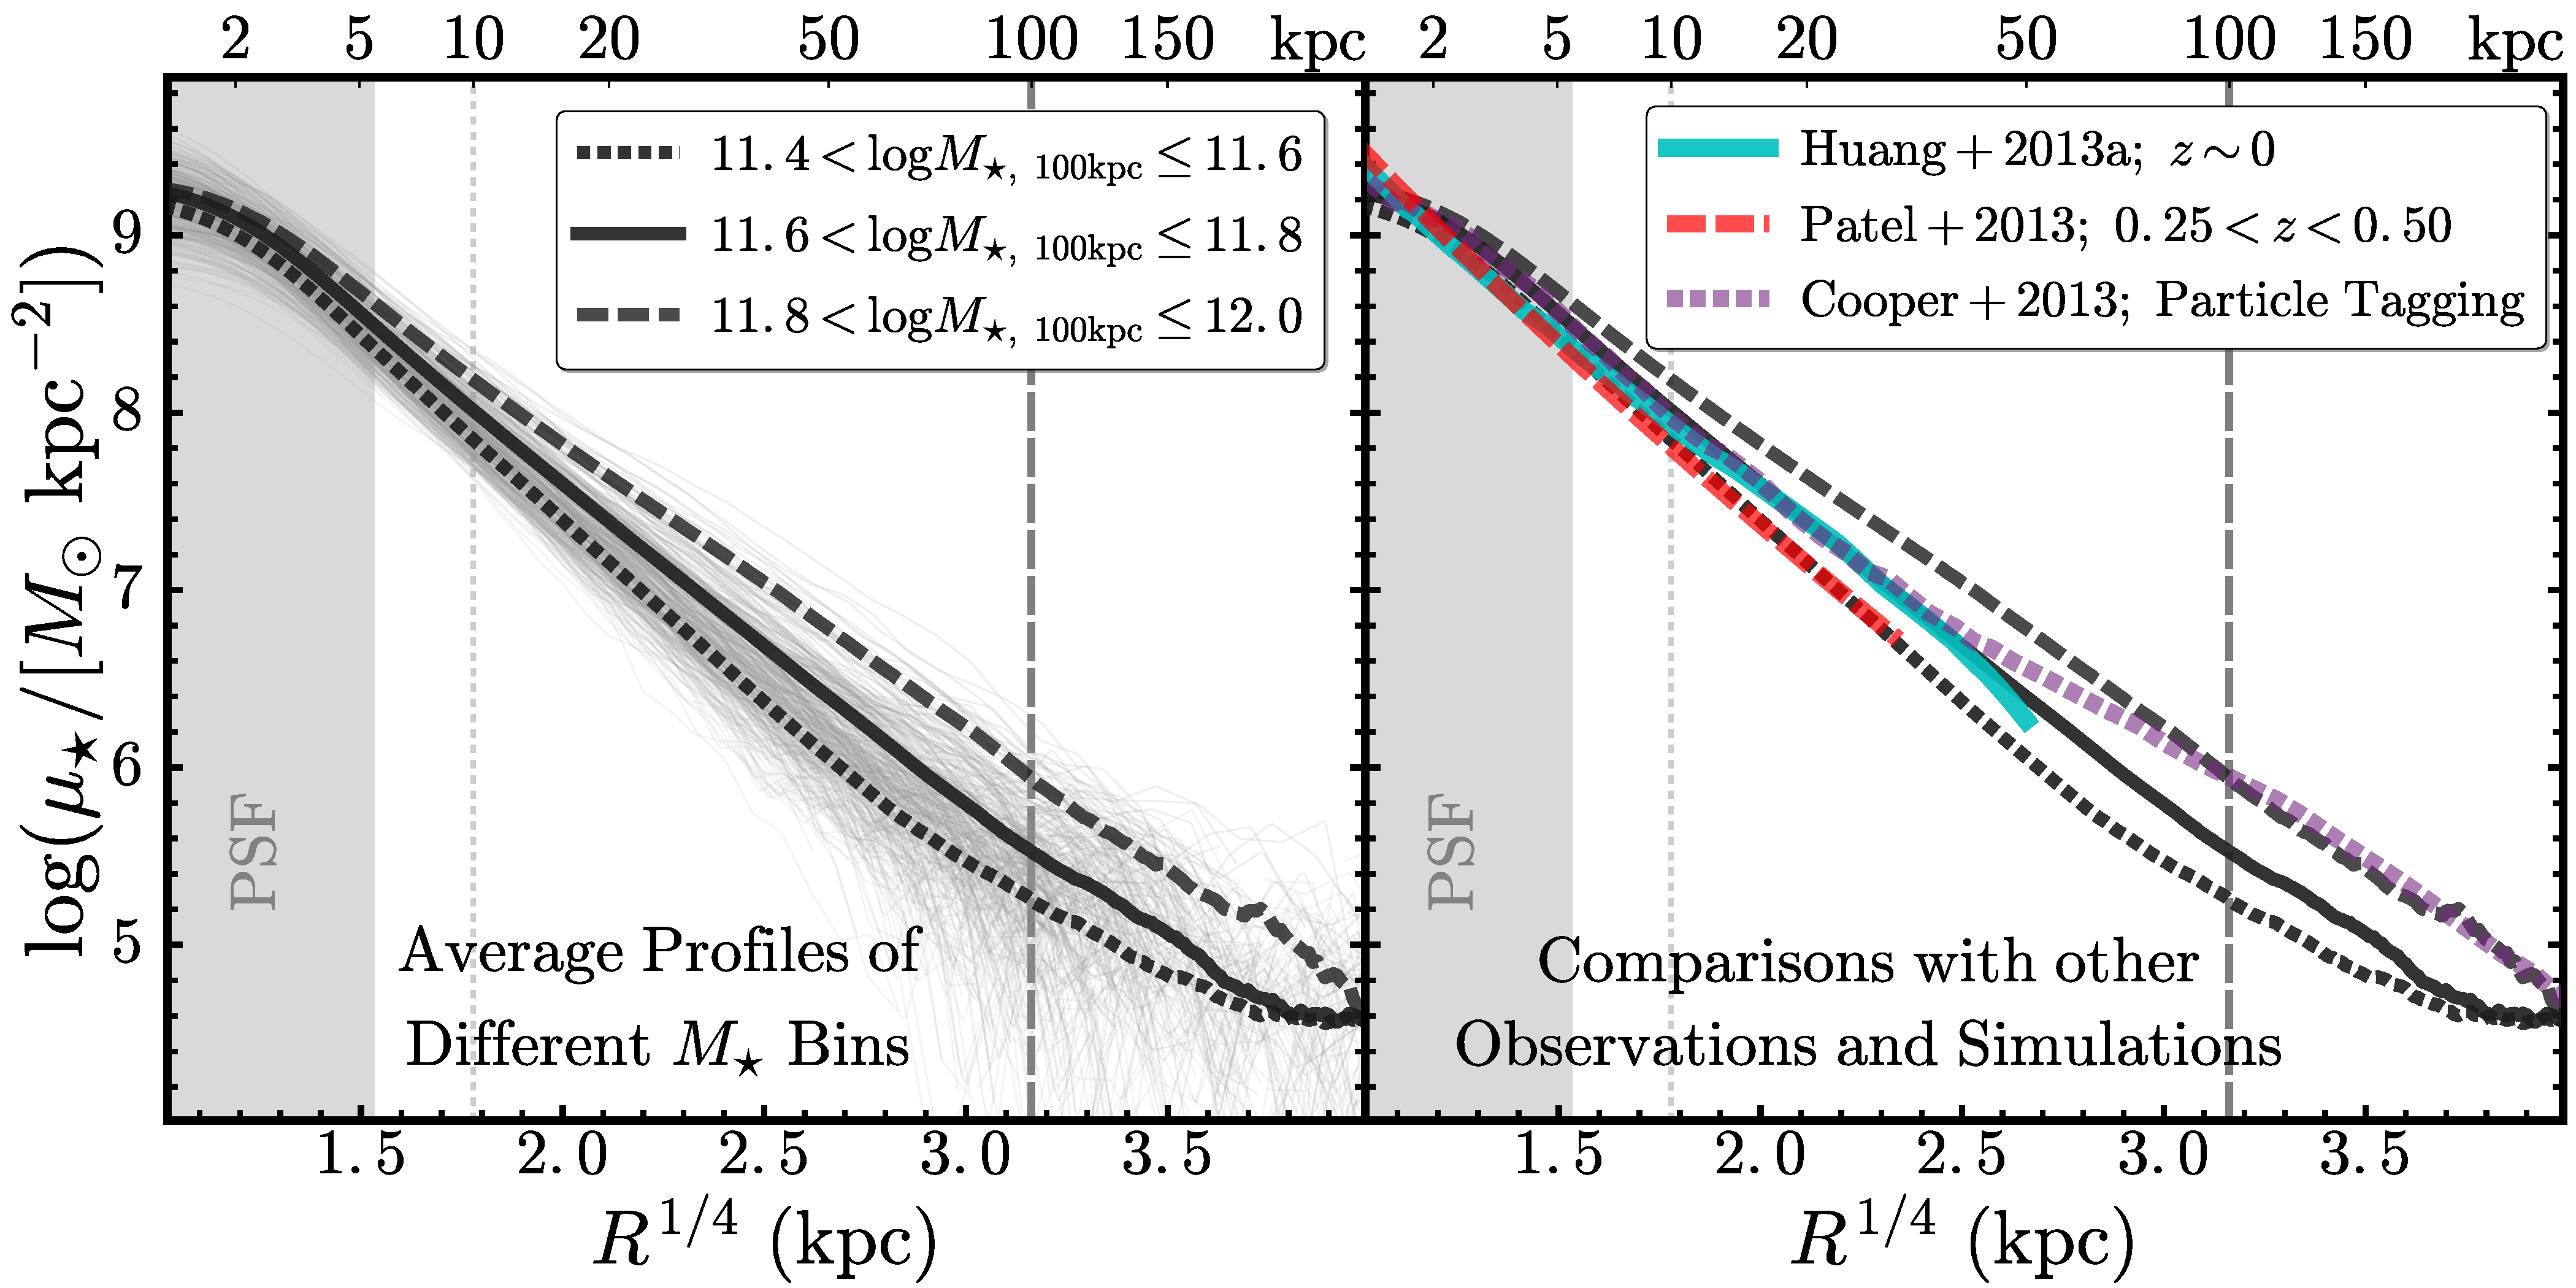
\includegraphics[width=\textwidth]{fig/average_mass_profiles_fsps1_A}
      \caption{
          \textbf{Left}: Median \mden{} profiles in three total stellar mass bins. 
              Thin grey lines show a random subset of individual profiles. 
              The shaded region highlights the region that could be affected by the PSF. 
              Two vertical lines indicate 10 kpc (thin, dotted line) and
              100 kpc (thick, dash line). ~~~ 
          \textbf{Right}: comparison between our \mden{} profiles, previous observations, 
              and simulations. 
              The solid cyan line shows the median profile of massive elliptical 
              galaxies at $z{\sim} 0$ from \citet[][]{Huang2013a}. 
              The red long-dashed line shows the median profile of massive galaxies at 
              $0.25 \leq z < 0.50$ observed by \textit{HST} from \citet[][]{Patel2013}. 
              The purple short-dashed line shows the median radial stellar distributions 
              in massive halos from simulation using the particle tagging method
              (\citealt{Cooper2013}).}
      \label{fig:avg_prof}
  \end{figure*}
%% ------------------------------------------------------------------------------------ %% 


%% ------------------------------------------------------------------------------------ %%
\subsubsection{General Trends and Comparison with Previous Work}
    \label{sssec:sbp_inter}
          
    Compared to the much discussed ``mass-size'' relation, the \mden{} profiles that 
    we have derived capture the full information about the structural properties of 
    massive galaxies. 
    We argue that by studying the shapes of these galaxy profiles directly, we can 
    by-pass outstanding questions about how to accurately define and measure the 
    ``sizes'' and ``masses'' of these massive galaxies. 
    Fig~\ref{fig:avg_prof} shows the median \mden{} profiles\footnote{The median 
    profiles along with their uncertainties are derived using bootstrap resampling 
    method} of massive central galaxies at $0.3 < z < 0.5$ in three \mtot{} 
    bins\footnote{The sample is clearly not complete in the lowest \mtot{} bin, 
    but its median \mden{} profile is still useful to show the overall trend and to 
    compare with previous work}. 
    As shown in the left panel of Fig~\ref{fig:avg_prof}, we can comfortably trace
    the \mden{} profiles of these massive galaxies out to 100 kpc 
    \textbf{individually}. 
    These median \mden{} profiles have moderate differences in the inner region, 
    but show significant differences in the outskirts with more massive galaxies 
    showing more prominent stellar envelopes. 
    \jenny{This seems out of place here:Most of these massive galaxies ($\ge 10^{11.4} M_{\odot}$) are slowly-rotating 
    (e.g.\ \citealt{Cappellari13b}) giant ellipticals with ``boxy'' inner isophotal 
    shapes (e.g.\ \citealt{Kormendy2009}), and slightly flattened inner \mden{} 
    profiles (e.g.\ \citealt{Lauer07})}. 
    But in the outskirts, the structure of these galaxies is 
    \emph{clearly not self-similar}. 
    Some of our \mden{} profiles show signs of unphysical truncation and fluctuation 
    related to inaccurate sky subtraction. 
    In this paper, we do not use profiles beyond 100 kpc, even though the median 
    \mden{} profiles for the two most massive bins behave reasonably out to 
    ${\sim} 200$ kpc. 
    
    Fig~\ref{fig:avg_prof} compares our results with previous work. 
    Most previous studies have relied on stacking techniques to measure surface 
    brightness profiles out to large radii.
    So far, the surface brightness profiles of massive galaxies out to such large 
    radii was mostly derived via image stacking technique that suffers from several 
    systematic issues (e.g. \citealt{Tal2011, DSouza2015}; but also see:
    \citealt{Capaccioli2015}); and the \mden{} profiles are even more rarely 
    available.
    
    \citet{Huang2013a} derived \mden{} profiles for a small sample of very nearby 
    ellipticals (within 100 Mpc; median \logms{} ${\sim} 11.3$ based on shallower 
    images) from the Carnegie-Irvine Galaxy Survey (CGS, \citealt{CGS1}). 
    Because this is a very low redshift sample, these profiles are robust to smaller scales, $r=1$ kpc. 
    The \citet{Huang2013a} profiles show good agreement with ours in the region of 
    overlap and out to 50 kpc. 
    CGS images are deeper than SDSS images in the $r$-band, but the median 
    profile from \citet{Huang2013a} still only reaches ${\sim} 50$ kpc for $z{\sim} 0$ 
    massive galaxies.
    Meanwhile, our deep HSC images can reliably deliver individual \mden{} profiles 
    for $z{\sim} 0.4$ galaxies out to at least 100 kpc.  
    
    \citet{Patel2013} extracted a median \mden{} profile of massive ETGs at 
    $0.25 < z < 0.50$ using stacked \textit{HST}/ACS images. 
    These galaxies are selected at a constant cumulative number density and are 
    thought to be the progenitors of $z=0$ massive ETGs (e.g. \citealt{Leja2013}).  
    The median \mstar{} of the \citet{Patel2013} sample is ${\sim} 10^{11.2} M_{\odot}$ 
    which is lower than our lowest mass bin. 
    However, \citet{Patel2013} use the BC03 SSP model which are roughly 0.1 dex 
    lower than our FSPS masses (Appendix~\ref{app:sed}). 
    Furthermore, the \citet{Patel2013} images are shallower than ours meaning 
    that there masses will be lower than ours because of missing light in the 
    outskirts. 
    Given these two considerations, it is reasonable to roughly compare the 
    \citet{Patel2013} profile with the one in our lowest stellar mass bin. 
    The superb resolution of the \textit{HST}/ACS image means that the profile in
    \citet{Patel2013} is unaffected by the seeing even down to 1 kpc. 
    The good agreement between our profile and the one derived from HST image 
    shows that our profiles are robust at $r > 3$ kpc and that we can accurately 
    measure \minn{}.
    
    Finally, we also compare with the predicted median \mden{} profile of central 
    galaxies in massive halos ($13.5 < \log M_{200,c} < 14.0$) from cosmological 
    simulation where the \mden{} profiles of galaxies are calculated using the 
    particle-tagging technique (e.g. \citealt{Cooper2010}). 
    
    The simulated \mden{} profile is also affected by limited resolution in the 
    center, but it is already quite similar to the median \mden{} profile for 
    the $11.6 <$ \logmtot{} $< 11.8$ bin within 40 kpc. 
    However, compared with our data, this simulation predicts stellar envelope that
    are too prominent at this halo mass. 
    This types of comparisons between our HSC data and predictions from simulations 
    will help to fine-tune simulations and to also investigate the main physical 
    mechanisms that drive the assembly of massive galaxies and the build up of 
    stellar envelopes.

    Table~1 provides tabulated values for the median profiles that are 
    displayed in Fig~\ref{fig:avg_prof}. 
    These profiles are also available  
    \href{https://github.com/dr-guangtou/hsc_redbcg/tree/master/profiles}{here}:
    {\url{https://github.com/dr_guangtou/hsc_redbcg/tree/master/profiles/}}.
    
%% ------------------------------------------------------------------------------------ %% 

%% ------------------------------------------------------------------------------------ %% 
\subsection{Ellipticity and Color Profiles}
    \label{ssec:ell_color}
    
%% ------------------------------------------------------------------------------------ %% 
  \begin{figure*}
      \centering 
      \includegraphics[width=\textwidth]{fig/redbcg_ell_color.pdf}
      \caption{
          Radial variations in ellipticity and optical colors for massive galaxies. 
          The format of this figure is similar to Fig~\ref{fig:avg_prof}. 
          \textbf{Left panel} shows the ellipticity profiles, 
          \textbf{Upper-right panel} shows the $g-r$ color profiles, and 
          \textbf{Lower-right panel} is for $g-i$ color profiles. 
          We compare our results with those from \citet{Tal2011} based on stacking 
          large samples of luminous red galaxies in SDSS at $z{\sim} 0.4$ 
          (solid red line on left panel). 
          We also compare with the results from a stacking analysis of nearby massive 
          galaxies with high concentration index ($C>2.6$) in 
          \citet[][blue dash lines on the left and upper-right panels]{DSouza2014}. 
          Finally, we also compare with the average $g-r$ and $g-i$ color profiles 
          from a large sample of nearby elliptical galaxies in \citet[][blue, solid 
          lines on both right panels]{LaBarbera2010}.
          }
      \label{fig:ell_color}
  \end{figure*}
%% ------------------------------------------------------------------------------------ %% 
    
%% ------------------------------------------------------------------------------------ %% 
	In addition to the shape of the light profile, we can also 
    study the $k$-corrected color profiles and ellipticity profiles 
    (computed via \texttt{Ellipse}) of these galaxies, and how 
    they depend on mass and environment.
    These quantities contain interesting information about the physical processes that 
    shape galaxies. We also want to be sure that we do not introduce any systematic bias in 
    our mass determinations because of systematic changes in color profile with stellar or 
    halo mass.
       
    %\begin{enumerate}
    %    
    %    \item To see whether the ellipticity profile depends strongly on environment, 
    %        and to see whether or not the fact that we use an using average isophotal 
    %        shape for our our 1-D \mden{} profiles has any impact on our results.
    %    
    %    \item To verify that the average color gradient does not depend strongly on 
    %        the environment and that is not steep enough to cause a problem with our 
    %        choice the assumption that it is reasonable to use average \m2l for 
    %        comparing massive galaxies. 
    %        We extract color profiles by applying the isophotes in $i$-band to images 
    %        in other bands in ``forced photometry'' manner.  
    %        
    %\end{enumerate}

    We compute ellipticities and color profiles in the radial range of 5-50 kpc 
    (this is the range where we can safely ignore differences in sky subtraction and 
    seeing across different bands). 
    We apply Galactic extinction and $k$-correction to both $g-r$ and $g-i$ color 
    profiles; the $k$-correction values are also from \texttt{iSEDFit} results.
    We show the average ellipticity, $g-r$, and $g-i$ color profiles for the 
    \mtot{}-matched (\minn{}-matched) samples of \rbcg{} and \nbcg{} galaxies on the 
    left (right) side of \ref{fig:ell_color}. 
    We also compare our results with previous work based on stacking SDSS galaxies 
    (e.g. \citealt{LaBarbera2010, Tal2011, DSouza2014}).
    
    We find that in general, the ellipticities of massive galaxies increases with 
    radius from $e\le 0.2$ around 5-10 kpc to $e{\sim} 0.3$ at 40-50 kpc. 
    This is consistent with previous 2-D modeling results from \citet{Huang2013a}. 
    The ellipticity profiles of the \mtot{}-matched samples are very similar at 
    $r<50$ kpc (2-3$\times R_{\mathrm{e}}$ for their \mstar{}). 
    However, for the \minn{}-matched samples, the \rbcg{} galaxies have higher 
    ellipticity than the \nbcg{} ones at $r > 10$ kpc, while their inner ellipticity 
    profiles are very similar.  
    This further hints that massive central galaxies in different halos but with 
    similar ``in-situ'' mass may experience different late-time merging histories. 
    Overall, the relative low ellipticity value and the fact that the ellipticity 
    gradients are shallow lead us to conclude that the use of an average 
    isophotal ellipticity is fine for this present study.
            
    Previous attempts to constrain ellipticity gradients have relied on image 
    stacking techniques (e.g. \citealt{Tal2011}, \citealt{DSouza2015}). 
    Compared to our measurements, we find that stacked ellipticity profiles tend to 
    underestimate the ellipticity in the outskirt. 
    Ellipticity profiles contain additional information about the assembly histories 
    and in future work, it would be of interest to compare our ellipticity profiles 
    with predictions from hydrodynamic simulations such as Illustris 
    (\citealt{Vogelsberger2014}, \citealt{Genel2014}) or \textit{Horizon-AGN} 
    (\citealt{Dubois2014}).
    
    In terms of color gradients, we find shallow and negative gradients of median 
    $g-r$ and $g-i$ color profiles for both \rbcg{} and \nbcg{} galaxies. 
    {\bf Can we also look as a function of stellar mass?}
    For both \mtot{}- and \minn{}-matched samples, we find no significant difference
    in their median color profiles, which supports the assumption of using single 
    average \m2l{} value to estimate \mden{} profiles.
    The median $g-r$ color profiles are quite consistent with those based on 
    stacked SDSS images. 
    For the $g-i$ profiles, the HSC ones show steeper gradients than the SDSS ones, 
    however, it is important to point out that the SDSS $i$-band suffers from the 
    so-called ``red-halo'' effect of (e.g. \citealt{Wu2005}, \citealt{Tal2011}) that 
    could make the SDSS color appears redder. 
    In contrast, HSC $i$-band image do not suffer from this effect (thanks to thick 
    CCDs), therefore can help provide more accurate color estimates.
%% ------------------------------------------------------------------------------------ %%
     

%% ------------------------------------------------------------------------------------ %% 
  \begin{figure*}
      \centering 
      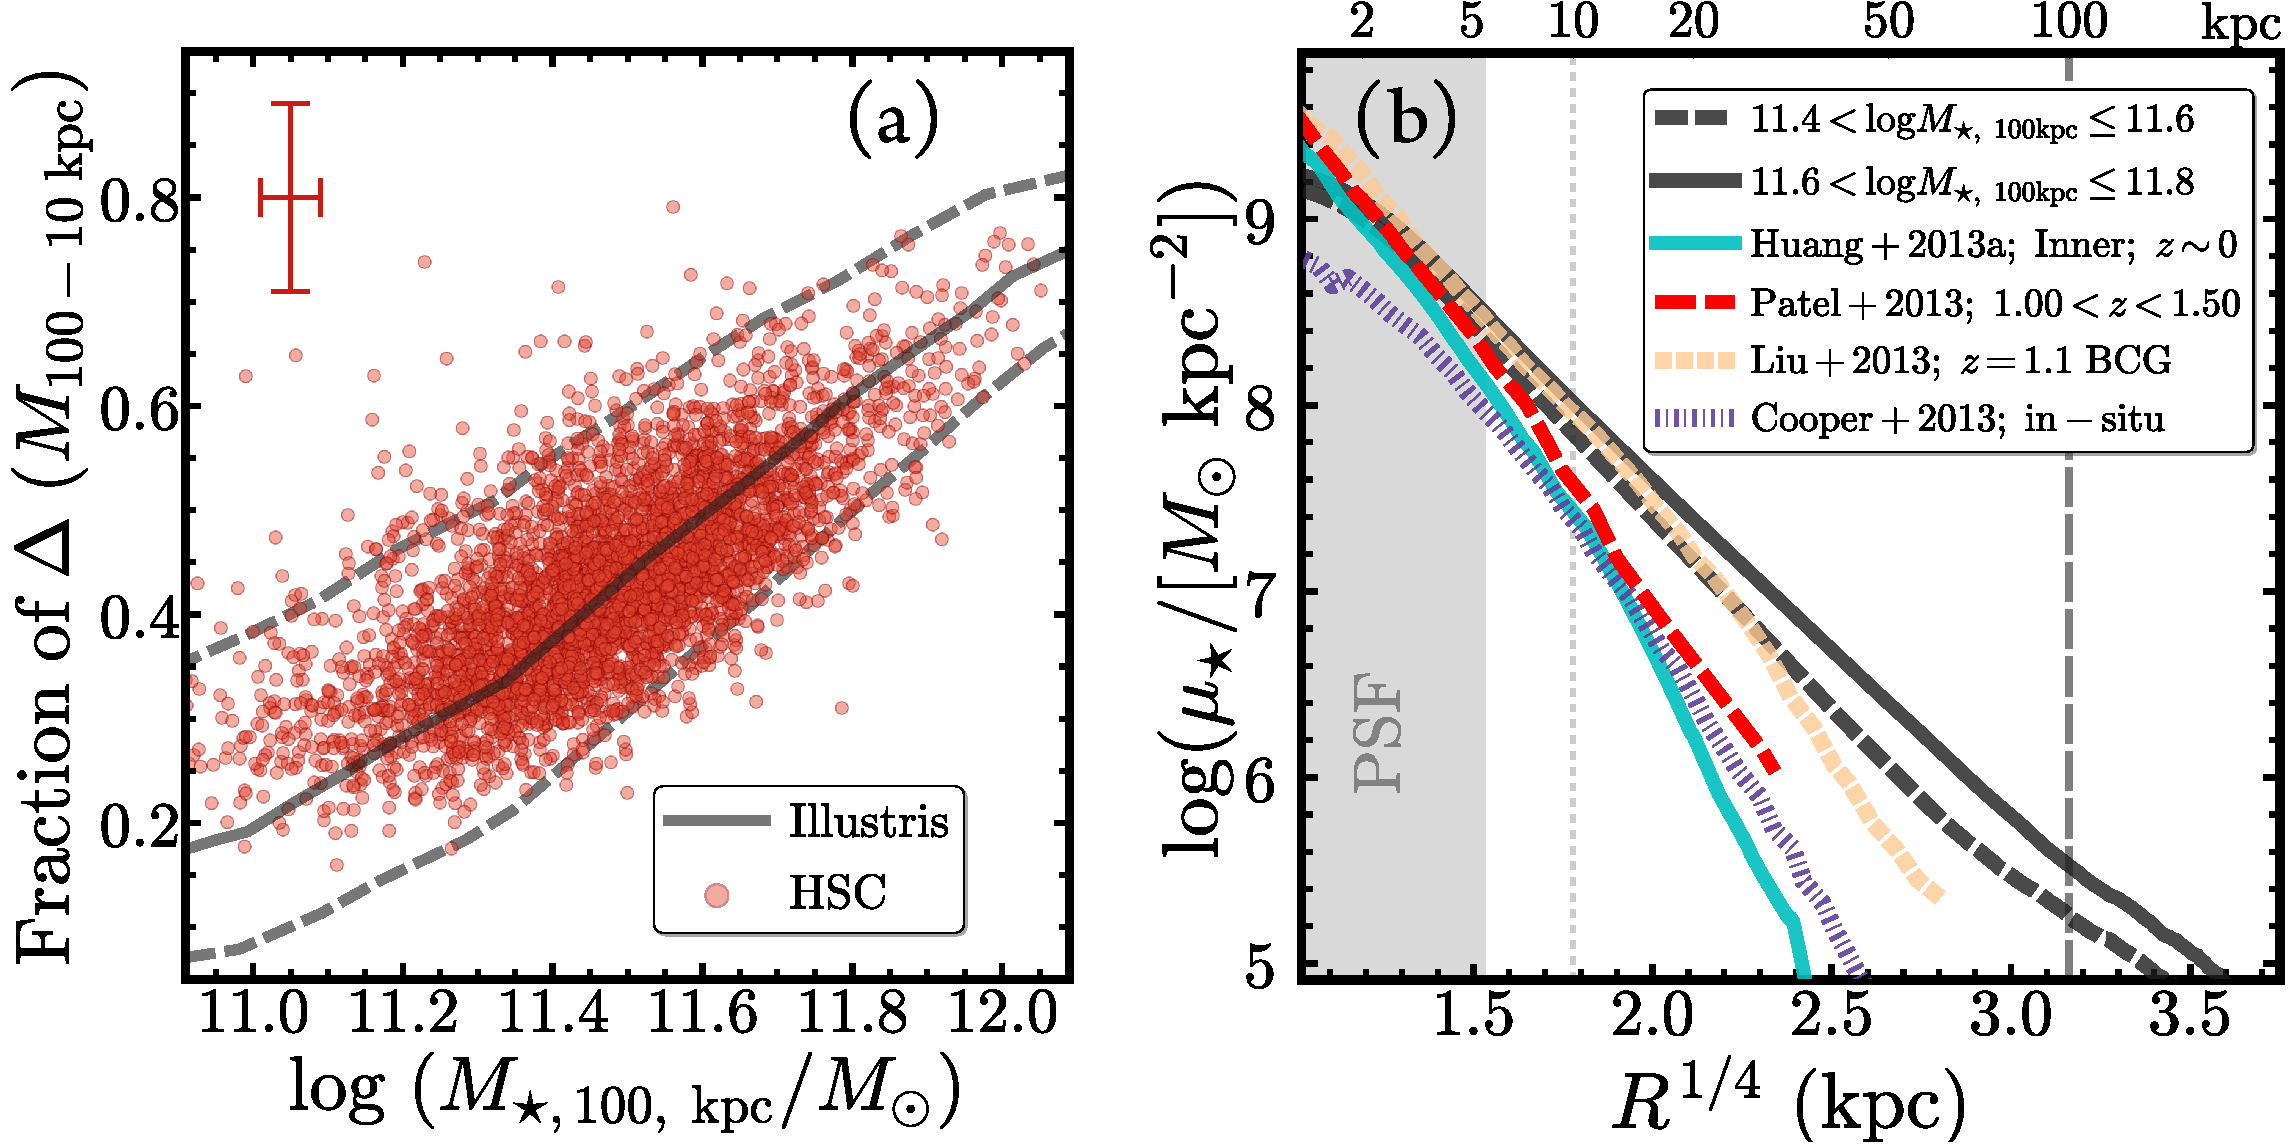
\includegraphics[width=\textwidth]{fig/redbcg_insitu_accretion}
      \caption{
          \textbf{Left:}
          Comparison of the median \mden{} profiles of massive galaxies in the 
          two lower \mtot{} bins from Fig~\ref{fig:avg_prof} with other observations 
          and simulations, focusing on the inner region. 
          The format is similar with the right panel of Fig~\ref{fig:avg_prof}.
          We include: 
          1) the median \mden{} profile of inner component from structure 
          decomposition of massive elliptical galaxies at $z{\sim} 0$ from 
          \citet[][Cyan, solid]{Huang2013a}; 
          2) the median \mden{} profile of massive galaxies at $1.0 < z < 1.5$ 
          from \textit{HST} observations in \citet[][Red, dashed]{Patel2013}; 
          3) the median \mden{} profile of the ``in-situ'' stellar components in 
          simulated massive halos from \citet[][Purple, dot-dashed]{Cooper2013};
          4) the \mden{} profile of the very massive cD galaxy at $z{\sim} 1.1$ 
          discovered by \citet[][Yellow, dashed]{Liu2013} in the Hubble 
          Ultra-Deep Field.
          \textbf{Right:}
          Relation between \mtot{} and the fraction of \mstar{} within 10 to 100 kpc, 
          which is used here as proxy of the fraction of accreted stars. 
          The typical uncertainties of \mtot{} and the mass fraction are shown in 
          upper-left corner. 
          This relation is compared with the relation between \mstar{} and the fraction
          of accreted stars derived from the Illustris simulation at $z=0$ 
          (Fig 4 in \citealt{RodriguezGomez2016}; grey solid and dashed lines). 
          }
      \label{fig:discussion_1}
  \end{figure*}
%% ------------------------------------------------------------------------------------ %% 

%% ------------------------------------------------------------------------------------ %% 
\section{Discussion}
    \label{sec:discussion}
    
    By using deep imaging from the HSC survey we have shown that the stellar mass 
    density profiles of massive central galaxies depend systematically on the mass 
    of their host dark matter halos. 
    Here we discuss the physical origin, scientific implications, and potential 
    caveats of this result. 
    
%% ------------------------------------------------------------------------------------ %% 
    
\subsection{The ``Two phase'' Formation Scenario of Massive Galaxies and the 
            Build-Up of Outer Envelopes}
    \label{ssec:twophase}

    {\bf Do we need two different sections and two different radial profile figures?}
            
    Our results are consistent with the picture that massive central galaxies form via 
    a ``two-phase'' scenario. 
    According to this theory, the cores of massive galaxies were formed at $z{\sim} 2$ 
    during an intense period of in-situ star formation. 
    The outskirts of massive galaxies are then built up via a more gradual second 
    phase of evolution (the ``ex-situ'' phase) which is dominated by mass growth via 
    the accretion of satellite systems. 
    Non-dissipative minor mergers mostly deposit stars on the outskirts of the 
    centrals and do not have large impact on the central \mden{} profile 
    (e.g. \citealt{Oogi2013, Bedorf2013}). 
    Hence, according to this picture, the outer stellar envelopes of massive centrals 
    should correlate with the masses of their host halos, in qualitative agreement with
    our findings. 
          
    State of the art hydrodynamic simulations suggest that massive dark matter halos 
    have central galaxies that have outer stellar envelopes with shallow slopes 
    (e.g. \citealt{Pillepich2014}). 
    This is consistent with the results in Fig \ref{fig:prof_1}.
     
    Meanwhile, these simulation also point out that the fraction of accreted stars 
    increases steeply with total \mstar{} and that the ``ex-situ'' component
    starts to dominate the \mden{} profiles around $R_{\mathrm{e}}$ for 
    \logms{}$\geq 11.5$ galaxies. 
    In this work, we find that the median \mden{} profiles of \rbcg{} and \nbcg{} 
    samples start to show differences around 15-20 kpc, which is close to 
    their $R_{\mathrm{e}}$. 
    Furthermore, the environmental dependence of our median \mden{} profiles 
    becomes more significant in our highest \mtot{} bin (see Fig \ref{fig:prof_4}). 
    These results all align with the picture that the \mhalo{}-dependence of the 
    \mden{} profiles of massive galaxies is driven by the variations in the 
    ``ex-situ'' component at large radii. 
   
    We now investigate to what degree our assumption that the inner 10 kpc \mstar{}
    corresponds to an in-situ mass.    
    Fig \ref{fig:discussion_1} compares the median \mden{} profiles of the 
    galaxies in two \mtot{} bins 
    ($11.4\leq$\logmtot{}$<11.6$ and $11.6\leq$\logmtot{}$<11.8$) with 
    (1) the median \mden{} profiles of massive ETGs at $1.0 < z < 1.5$ in
    \citealt{Patel2013} since they are considered as the progenitors of 
    ${\sim} 10^{11.5} M_{\odot}$ ETGs at $z=0$.    
    (2) the inner components of $z{\sim} 0$ ellipticals from 2-D decomposition 
    (\citealt{Huang2013a}).
    As proxy of the in-situ components, \citet{Huang2013b} showed they are 
    structurally similar to the compact ``red nuggets'' at high-$z$. 
    (3) the ``in-situ'' components of simulated central galaxies in massive halos 
    from \citet{Cooper2013} (the inner ${\sim} 5$ kpc is quite uncertain due to the 
    resolution).  
    The comparison confirms that \minn{} should be reasonable proxy of the 
    ``in-situ'' mass\footnote{We convert these \mden{} profiles to the same 
    Chabrier IMF; but there are still differences in median \mstar{} and 
    details in the \m2l{} estimates}.  
    More importantly, it shows that the \mden{} profile at 
    $\mathrm{R} > 15$-20 kpc is likely dominated by stars that are not related 
    to the ``in-situ'' processes.  
    
    We also compare with a uniquely massive BCG at high redshift: 
    a ${\sim} 10^{11.4} M_{\odot}$ BCG with distinctive ``cD''-like envelope at 
    $z{\sim} 1.1$ (\citealt{Liu2013}).  
    Its \mden{} profile follows the median profile of $11.6\leq$\logmtot{}$<11.8$ 
    massive galaxies nicely inside 10-15 kpc, but becomes much steeper in the outskirt.  
    This unique object may present an interesting case where the inner ``core'' of a 
    massive BCGs is already in pace at $z{\sim} 1$ when its extended envelope is still
    under construction.
    More BCGs like this at $0.5 < z < 1.0$ can shed light on this intriguing 
    process, and help us confirm whether the environmental dependence of structure 
    has already emerged within massive galaxies at higher redshift 
    (e.g. \citealt{Papovich2012})
    
    {\bf Have we looked at delta M as a function of Mtot?  I think that would be useful 
    for comparison with the Oser papers, for instance. }

%% ------------------------------------------------------------------------------------ %% 

%% ------------------------------------------------------------------------------------ %% 
  \begin{figure*}
      \centering 
      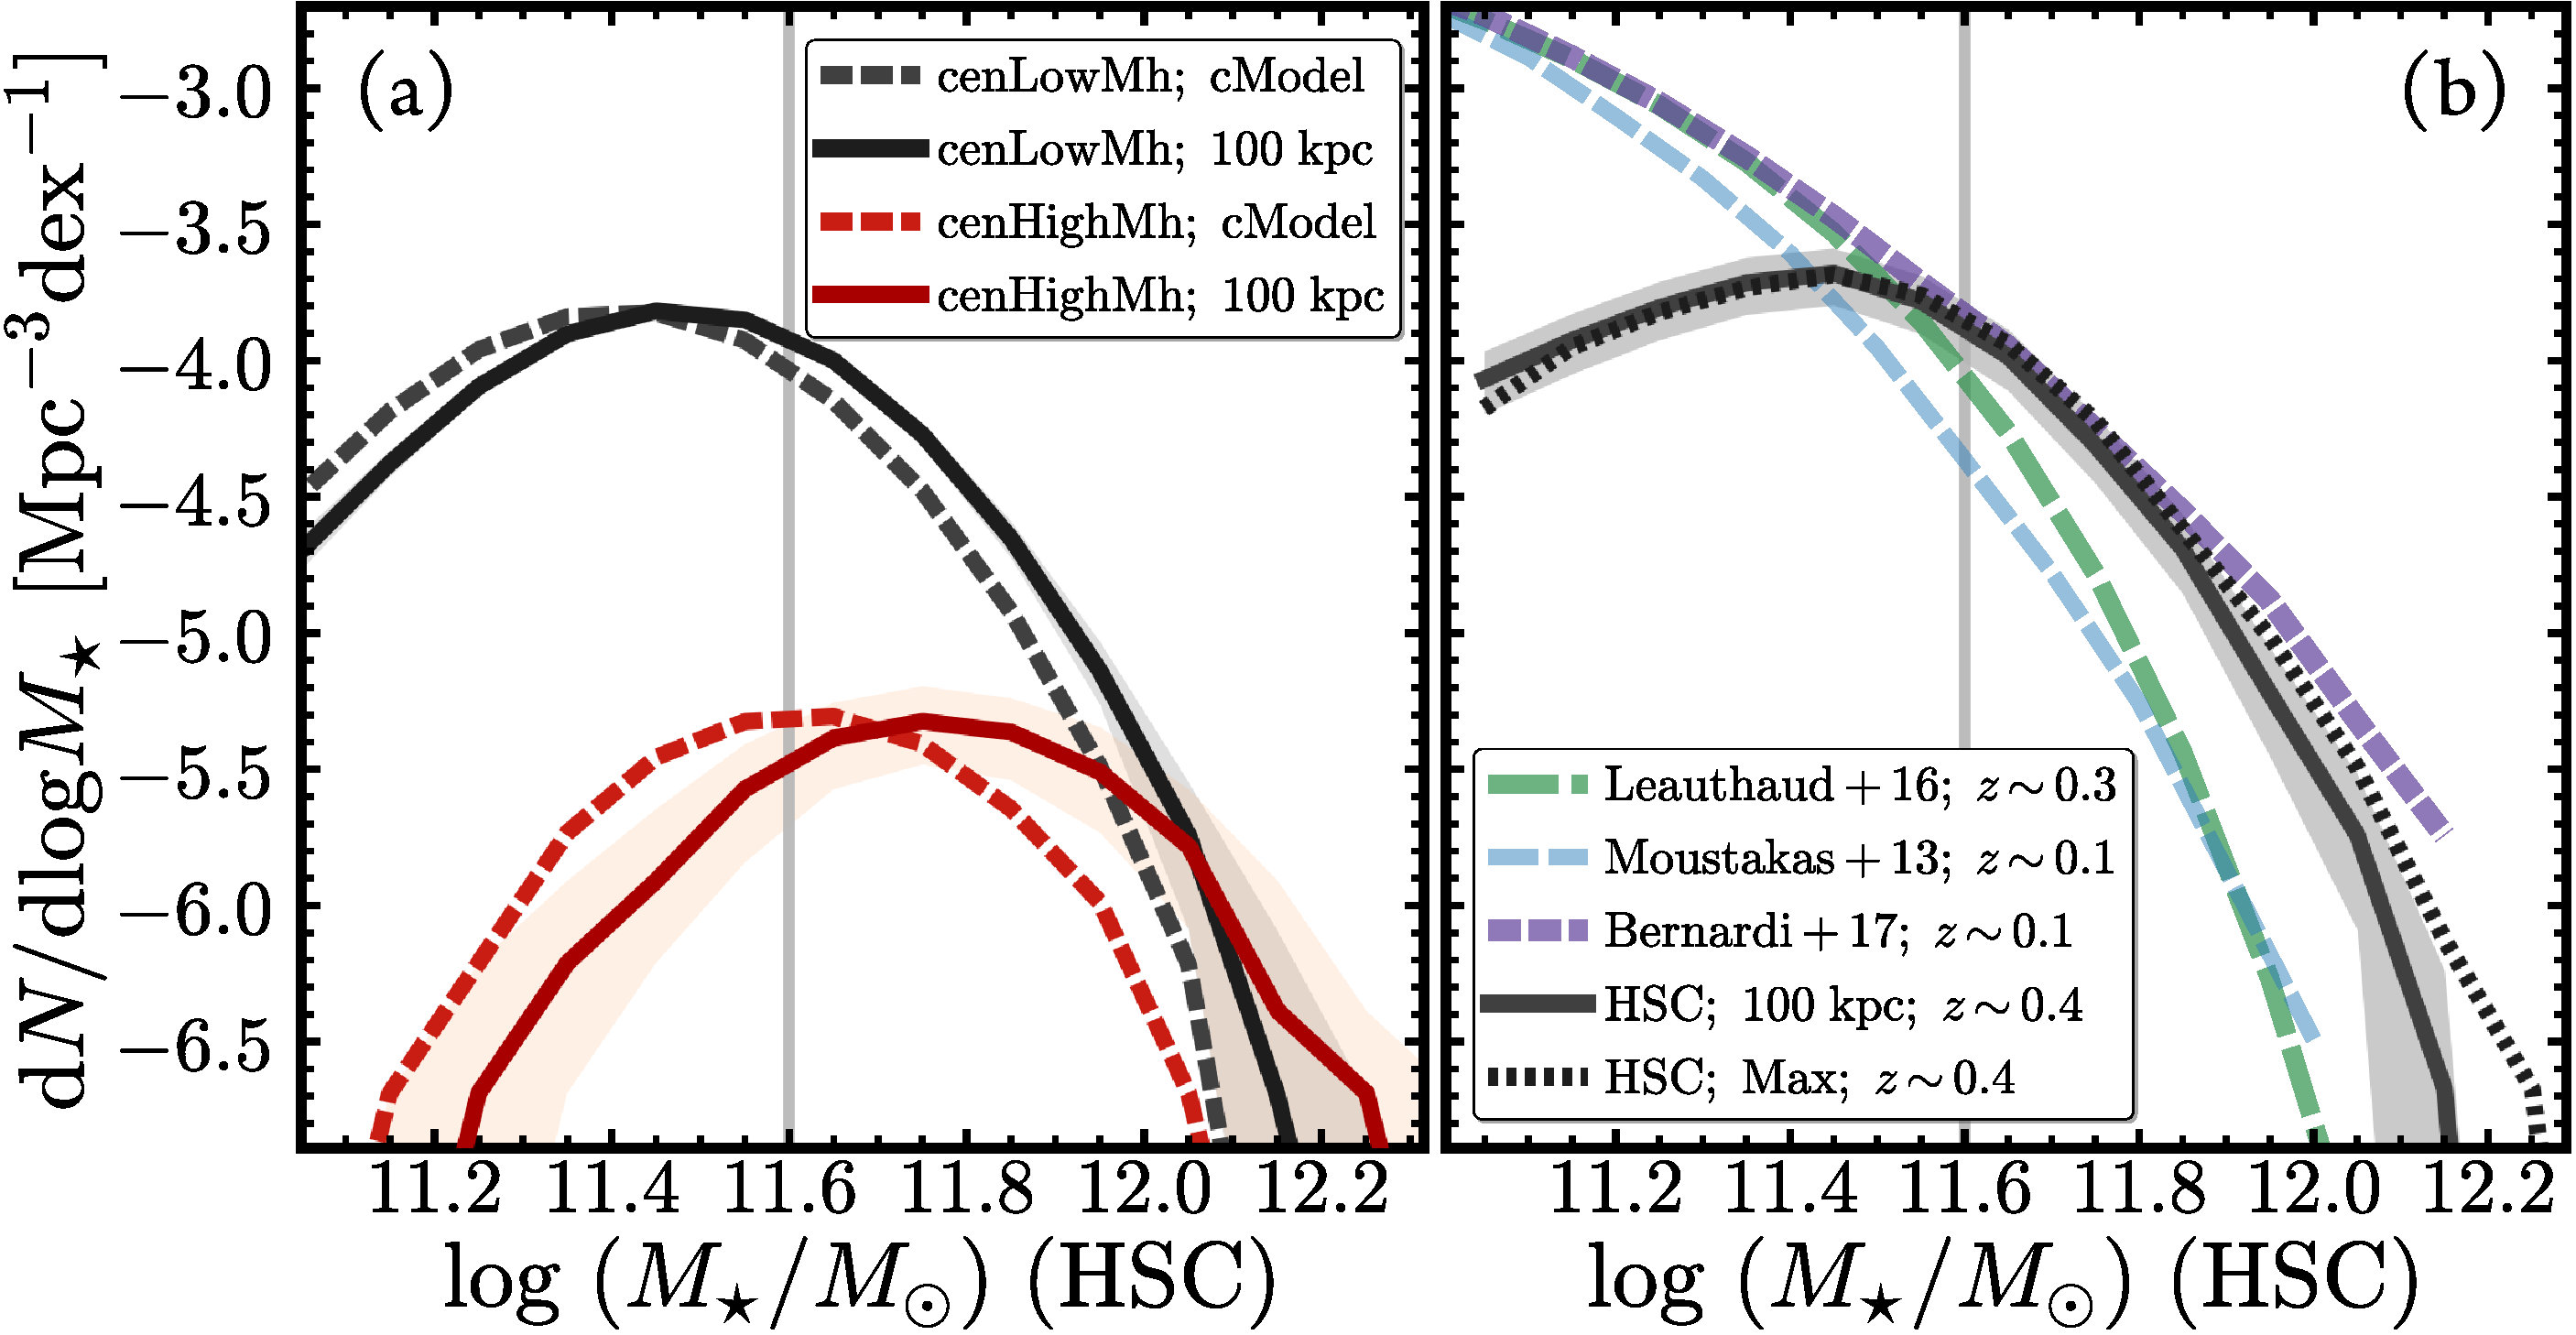
\includegraphics[width=\textwidth]{fig/redbcg_mass_smf}
      \caption{
          \textbf{Left:} Impact of using \mtot{} on the galaxy stellar mass function. 
          Dashed lines correspond to the SMF computed using \mcmodel{} whereas solid 
          lines correspond to the SMF computed using \mtot{}. 
          Here we separate the HSC massive galaxies into the central galaxies living 
          in halos more massive than \logmh{}$\sim14.2$ (red lines) and the ones in 
          halos with \logmh{}$<14.0$ (black lines).
          The impact on the SMF can exceed 0.2 dex for massive central galaxies in 
          very massive halos.
          \textbf{Right}: The stellar mass volume density distributions of massive 
          HSC galaxies, using both \mtot{} (black solid line) and \mmax{} (black dotted 
          line). 
          The uncertainty of distribution using \mtot{} is shown in grey shaded 
          region.  
          Here, we also compare the distributions with SMF from previous works: 
          (a): SDSS galaxies at $z{\sim} 0.1$ from \citet{Bernardi2013}; the \mstar{} 
          is based on photometry from 2-D \ser{}$+$Exponential model fitting 
          (purple); 
          (b): SDSS galaxies at $z{\sim} 0.1$ from \citet{Moustakas13} based on 
          improved SDSS \texttt{cModel} photometry (blue); 
          (c): \texttt{S82-MGC} galaxies at $0.15 < z< 0.43$ from 
          \citet{Leauthaud2016} based on PSF-matched SDSS-UKIDSS photometry (green).
          Please see text for more details of the comparison.
          }
      \label{fig:discussion_2}
  \end{figure*}
%% ------------------------------------------------------------------------------------ %%

%% ------------------------------------------------------------------------------------ %% 
\subsection{What is the ``Total Mass'' of Massive Galaxies?}

    Even with deep HSC images, it is non trivial to clearly define and measure the
    ``total'' \mstar{} for these massive systems. 
    As discussed in Section~\ref{ssec:mtotal}, our 1-D approach has certain advantages 
    over the 2-D modeling method and in principle, should capture a the majority of 
    the stellar mass. 
    However, even though we extend to 100 kpc, there is no evidence that the profile 
    drops to zero on these scales. 
    We now estimate how much extra mass is ``hidden'' beyond the 100 kpc radius. 
    For this, we integrate the \mden{} profiles out to the detection limit in 
    surface brightness profile that is defined by the background noise.
    We will call this the ``maximum mass'' of the galaxy (\mmax{}). 
    For obvious reasons, we find that \mmax{} is larger than \mtot{} with an average 
    difference of about ${\sim}0.04$ dex. 
    The left hand side of Fig \ref{fig:discussion_2} shows differences between \mtot{}
    and \mmax{}. 
    On a galaxy-by-galaxy basis, the difference \mmax{}-\mtot{} depends on the slope 
    of the stellar envelope. 
    In this work, we have opted to in general use \mtot{} rather than \mmax{} as the 
    uncertainty on \mmax{} is larger. 
    However, we have checked that none of our results are changed by replacing \mtot{} 
    via \mmax{}.
        
    How to define and measure the ``total'' mass of a galaxy becomes a critical 
    question when studying the high-mass end of the galaxy SMF. 
    The issues discussed above are currently one of the primary limitations in 
    determinations of the high-mass end of the SMF (\citealt{Bernardi2016}). 
    Fig~\ref{fig:mass_complete} illustrated how improved \mstar{} measurement can 
    significantly modifies the SMF. 
    On the right hand side of Fig~\ref{fig:discussion_2}, we further highlight that 
    the shape of SMF at high-mass end is quite sensitive to even very small 
    change of \mstar{}. 
    We also compare the SMFs of our HSC samples with the following previous studies:
        
    \begin{itemize}
    
        \item The SMF derived from a SDSS-\textit{GALEX} sample of $z{\sim} 0.1$ 
            galaxies from \citet{Moustakas13}. 
            Here, the total luminosity is based on the SDSS \cmodel{} magnitude. 
            The \m2l{} is derived via SED fitting using \texttt{iSEDfit} with similar 
            assumptions as in our work.
            
        \item The SMF for $z{\sim} 0.1$ SDSS galaxies from \citet{Bernardi2013}. 
            The total luminosity is based on 2-D \texttt{SerExp} models 
            (\ser{}$+$ Exponential disk model; integrated to infinity) that 
            recovers much more flux compared to SDSS \cmodel{} magnitudes. 
            The \m2l{} is also from SED fitting assuming a Chabrier IMF.
            
        \item The SMF for $0.15 < z < 0.30$ galaxies from the \texttt{S82-MGC} sample
            \citep{Leauthaud2016} where the \mstar{} is derived using 
            \texttt{iSEDfit} on PSF-corrected aperture photometry from 
            \texttt{S82}.
            
    \end{itemize}

%% ------------------------------------------------------------------------------------ %% 
    It is clear that different analyses lead to very different slopes at high-mass end. 
    Here, we do not try to evaluate whether the differences displayed in 
    Fig~\ref{fig:discussion_2} are dominated by differences in photometry versus 
    assumptions about stellar population models (e.g. \citealt{Bernardi2016}). 
    However, given that the results that we are comparing assume the same IMF and adopt 
    similar assumptions about stellar population models, we hypothesize that the 
    differences in Fig~\ref{fig:discussion_2} are dominated by differences in photometry. 
    The goal of our of present paper is not to present and discuss a careful evaluation
    of the high-mass end of the SMF -- this will be presented in a forthcoming paper 
    once the HSC survey has accumulated more data. 
    However, this is clearly a topic that warrants further investigation, and careful 
    photometry measurements from HSC data will shed further light on these questions.     
      
    Finally, we emphasize that in this present study we do not attempt to separate the 
    light of the galaxy with a potential (and distinct) ``intra-cluster''
    light component (ICL; e.g. \citealt{Carlberg1997, Lin2004, Gonzalez2005, 
    Mihos2005}). 
    Instead, we adopt the view that the light of the main galaxy and the 
    ``intra-cluster''component are a smooth and continuous distribution. 
    A reliable isolation of a physically meaningful ICL component using photometry 
    alone is extremely difficult, if not impossible. 
    At the imaging depth of HSC, we find no evidence for a clearly distinction between 
    an ``inner component'' and an ``intra-cluster'' component. 
    Instead, most of our profiles are smoothly varying out to 100 kpc with little 
    evidence for a distinct secondary component. 
    We do note however, that our \rbcg{} sample contains only a small fraction of 
    extremely massive clusters where strong evidence of photometric ICL component is 
    often found (\mhalo{}$\simgt 10^{15}M_{\star}$). 
    At the typical \mhalo{} of our \rbcg{} clusters, one good nearby example would be 
    the Virgo cluster, whose ultra-deep images (e.g. \citealt{Mihos2016}) show
    that the stellar halo of the BCG can smoothly extends beyond 100 kpc, while the 
    ICL only becomes important outside that radius and is dominated by individual 
    tidal features. {\bf I continue to think you are saying all gals have some ICL, rather 
    that no galaxies have ICL...}

%% ------------------------------------------------------------------------------------ %% 

%% ------------------------------------------------------------------------------------ %% 
\section{Summary and Conclusions}
    \label{sec:summary}

    In this work, we study how environment (halo mass) affects the stellar mass density 
    profiles of massive central galaxies using deep images from the Subaru HSC 
    survey. 
    With the help of this high-quality and wide area data set, we directly map the 
    stellar mass distributions of ${\sim}7000$ massive central galaxies at 
    $0.3 < z < 0.5$ out to $>100$ kpc without resorting to stacking techniques. 
    We group massive central galaxies into two categories based on their host halo 
    mass (\mhalo{}$\simgt 10^{14.2} M_{\odot}$ and \mhalo{}$\simlt 10^{14} M_{\odot}$). 
    Our main results are:  
    
    \begin{enumerate}
        \item We find that the ``total'' \mstar{} of these massive galaxies can be 
            significantly underestimated with shallow imaging data such as SDSS and/or 
            imperfect model assumption (e.g. the \texttt{cModel} or single-\ser{}) 
            are used. 
            In contrast to previous work, our results do not depend on stacking or any 
            parametric models. 
            Moreover, the level of such underestimation could also depend on the 
            stellar mass and on halo mass. 
            This should be carefully taken into account when discussing topics such 
            as the evolution of the galaxy SMF.
            
        \item We show that the \mden{} profiles of massive galaxies are generally quite 
            smooth out to 10 kpc but that there is a large but continuous scatter in the 
            amount of light in their outskirts. 
            {\bf KEEP? We argue that ``cD'' galaxies simply represent the tail end of a 
            distribution but that they are not a distinct class of massive galaxies.}
            
        \item {\bf How do profiles depend on Mstar?}
            
    \end{enumerate}

    These results highlight the advantages of wide area, deep, and high-quality imaging 
    for studying the evolution of massive galaxies. 
    Upon finishing this work, the HSC survey has already doubled its sky coverage to 
    ${\sim} 200$ deg$^2$, and provides a much larger sample of massive central galaxies. 
    In the near future, we will extend this work to lower \mtot{} by using photometric 
    redshifts, and we will also apply 2-D photometry method (e.g.\ \citealt{Huang2013a}) 
    to take advantages of the multi-wavelength nature of the HSC survey 
    (e.g. \citealt{Huang2016}). 
    Our current work can also be combined with weak lensing measurements of the dark 
    matter halos of massive galaxies and physical insights into the assembly histories 
    of these galaxies can be gained by comparing with cosmological hydro-simulations 
    such as Illustris (\citealt{Vogelsberger2014}, \citealt{Genel2014}), 
    EAGLE (\citealt{Schaye2015}, \citealt{Crain2015}), or \textit{Horizon-AGN} 
    (\citealt{Dubois2014}).

%% ------------------------------------------------------------------------------------ %% 
  
\section*{Acknowledgements}

  % Personal 
  SH thanks F.S.Liu for sharing the data from his work.

  % HSC part
  The Hyper Suprime-Cam (HSC) collaboration includes the astronomical communities of 
  Japan and Taiwan, and Princeton University.  The HSC instrumentation and software were
  developed by the National Astronomical Observatory of Japan (NAOJ), the Kavli Institute
  for the Physics and Mathematics of the Universe (Kavli IPMU), the University of Tokyo,
  the High Energy Accelerator Research Organization (KEK), the Academia Sinica Institute
  for Astronomy and Astrophysics in Taiwan (ASIAA), and Princeton University.  
  Funding was contributed by the FIRST program from Japanese Cabinet Office, the Ministry 
  of Education, Culture, Sports, Science and Technology (MEXT), the Japan Society for 
  the Promotion of Science (JSPS), Japan Science and Technology Agency (JST), the
  Toray Science Foundation, NAOJ, Kavli IPMU, KEK, ASIAA, and Princeton University.
   
  % SDSS part
  Funding for SDSS-III has been provided by the Alfred P. Sloan Foundation, the
  Participating Institutions, the National Science Foundation, and the U.S.  Department of
  Energy. The SDSS-III web site is http://www.sdss3.org.  SDSS-III is managed by the
  Astrophysical Research Consortium for the Participating Institutions of the SDSS-III
  Collaboration including the University of Arizona, the Brazilian Participation Group,
  Brookhaven National Laboratory, University of Cambridge, University of Florida, the
  French Participation Group, the German Participation Group, the Instituto de Astrofisica
  de Canarias, the Michigan State/Notre Dame/JINA Participation Group, Johns Hopkins
  University, Lawrence Berkeley National Laboratory, Max Planck Institute for
  Astrophysics, New Mexico State University, New York University, Ohio State University,
  Pennsylvania State University, University of Portsmouth, Princeton University, the
  Spanish Participation Group, University of Tokyo, University of Utah, Vanderbilt
  University, University of Virginia, University of Washington, and Yale University.
  
  % Pan-STARRS1 part
  The Pan-STARRS1 Surveys (PS1) have been made possible through contributions of the 
  Institute for Astronomy, the University of Hawaii, the Pan-STARRS Project Office, 
  the Max-Planck Society and its participating institutes, the Max Planck Institute 
  for Astronomy, Heidelberg and the Max Planck Institute for Extraterrestrial Physics, 
  Garching, The Johns Hopkins University, Durham University, the University of Edinburgh, 
  Queen's University Belfast, the Harvard-Smithsonian Center for Astrophysics, the Las 
  Cumbres Observatory Global Telescope Network Incorporated, the National Central 
  University of Taiwan, the Space Telescope Science Institute, the National Aeronautics 
  and Space Administration under Grant No. NNX08AR22G issued through the Planetary 
  Science Division of the NASA Science Mission Directorate, the National Science 
  Foundation under Grant No. AST-1238877, the University of Maryland, and Eotvos 
  Lorand University (ELTE).
  
  % LSST software
  This paper makes use of software developed for the Large Synoptic Survey 
  Telescope. We thank the LSST Project for making their code available as free 
  software at http://dm.lsstcorp.org.
 
  % Software
  This research made use of:
  \href{http://www.stsci.edu/institute/software_hardware/pyraf/stsci\_python}{\texttt{STSCI\_PYTHON}},
      a general astronomical data analysis infrastructure in Python. 
      \texttt{STSCI\_PYTHON} is a product of the Space Telescope Science Institute, 
      which is operated by AURA for NASA;
  \href{http://www.scipy.org/}{\texttt{SciPy}},
      an open source scientific tools for Python (\citealt{SciPy});
  \href{http://www.numpy.org/}{\texttt{NumPy}}, 
      a fundamental package for scientific computing with Python (\citealt{NumPy});
  \href{http://matplotlib.org/}{\texttt{Matplotlib}}, 
      a 2-D plotting library for Python (\citealt{Matplotlib});
  \href{http://www.astropy.org/}{\texttt{Astropy}}, a community-developed 
      core Python package for Astronomy (\citealt{AstroPy}); 
  \href{http://scikit-learn.org/stable/index.html}{\texttt{scikit-learn}},
      a machine-learning library in Python (\citealt{scikit-learn}); 
  \href{http://www.astroml.org/}{\texttt{astroML}}, 
      a machine learning library for astrophysics (\citealt{astroML});
  \href{https://ipython.org}{\texttt{IPython}}, 
      an interactive computing system for Python (\citealt{IPython});
  \href{https://github.com/kbarbary/sep}{\texttt{sep}} 
      Source Extraction and Photometry in Python (\citealt{PythonSEP});
  \href{https://jiffyclub.github.io/palettable/}{\texttt{palettable}},
      color palettes for Python;
  \href{http://dan.iel.fm/emcee/current/}{\texttt{emcee}}, 
      Seriously Kick-Ass MCMC in Python;
  \href{http://bdiemer.bitbucket.org/}{\texttt{Colossus}}, 
      COsmology, haLO and large-Scale StrUcture toolS (\citealt{Colossus}).

%%%%%%%%%%: Bibliographic Section %%%%%%%%%%

\bibliographystyle{mnras}
\bibliography{redbcg}

%%%%%%%%%%: Appendix Section %%%%%%%%%%%%

\appendix
    
%% ------------------------------------------------------------------------------------ %% 
\section{A. Extraction of 1-D surface brightness profile} 
    \label{app:ellipse} 
    
    Here we briefly discuss a few technical issues related to the measurements of the 
    1-D surface brightness profiles around massive galaxies. 
    
    To derive reliable 1-D profile, it is important to mask out all the irrelevant 
    objects around the target.
    At the depth of the HSC images, this becomes a challenging task, especially 
    for massive galaxies with extended outer profiles and many satellites. 
    At this point, the \texttt{hscPipe} tends to over-subtract the background around 
    bright objects.  
    The performance of its deblending process is also not optimized for extended
    objects. 
    For these reasons, we perform \texttt{SExtractor}-like background subtraction and 
    object detection using the \texttt{SEP} Python library to generate the necessary 
    masks.
    Combining two different local background models and $S/N$ thresholds, we obtain 
    the centroid, shape, and radius that enclose 90\% of flux for each object, 
    including the one that is very close to the center of bright galaxy (left panel of 
    Fig~\ref{fig:ell_tech}). 
    Based on these information, we then create the mask that covers all contaminating 
    objects around the target after adaptively increasing the sizes of their masks 
    according to their brightness and distance to the central target. 
    Generally speaking, we mask out bright objects or objects in the outskirt of the 
    image more aggressively to reduce their impact on the surface brightness profiles 
    in the outskirt. 
    We also create masks that are less and more aggressive than the default one to 
    test their impacts on the surface brightness profiles. 
    
    Next, we aggressively mask out all objects on the cut-out image.  
    We then evaluate the background level using the unmasked pixels after median 
    smoothing the masked image using box of $6x6$ pixels.
    This provides estimate of global background level along with its uncertainty. 
    Given the typical background uncertainty, the HSC \texttt{WIDE} image should be 
    able to reach down to $> 29$ \sb surface brightness level in the $i$-band.  
    However, as mentioned, we often find evidence of slightly over-subtracted 
    background for massive galaxies in our sample. 
    In the current \texttt{hscPipe}, the background on each CCD is modeled with a 
    Chebyshev-polynomial that is fit to the smoothed image after excluding pixels 
    with $S/N >5$.
    This algorithm performs much better than the SDSS version 
    (e.g.\ see \citealt{Blanton2011}), yet still over-subtracts background around 
    bright objects and results in unphysical truncation in their surface brightness 
    profiles.
    We empirically correct this issue using the background model generated by 
    the \texttt{SExtractor} algorithm on the masked image 
    ($200x200$ pixels background box size, and 6 pixels median filtering size of 
    sky boxes).
    This model can account for the slightly over-subtracted background at large scale,
    and reduce the impact from the low surface brightness ``wings'' of bright 
    neighbors. 
    We clearly see improvement in both the distributions of background pixels 
    (more symmetric distribution; median value is closer to 0) and the surface 
    brightness profile (middle panel of Fig~\ref{app:ellipse}; the negative intensity 
    and the turn-over of the curve-of-growth in the outskirt of the ``Original'' 
    profile are successfully corrected) after this correction.
    Also, it is worth mentioning that such correction does not often affect the 
    surface brightness profile within 100 kpc. 
    
    The procedure used to derive 1-D surface brightness profile from the 
    background-corrected, contamination-masked images is already described in 
    Section~\ref{sec:ellipse} briefly. 
    In practice, the profile at very low surface brightness level is sensitive to 
    several \texttt{Ellipse} configurations.
    After some tests, we choose to use 0.1 dex in logarithm as the step in semi-major 
    axis length between successive ellipses, and we use the median pixel value over the
    elliptical annulus after rejecting outlying pixels via $3\sigma$-clipping three
    times.
    We make the above choices to make the final profile less affected by any nearby
    object, and also test the differences between the profiles derived using larger
    step, or mean value on the annulus, or fewer times of $\sigma$-clipping. 
    Generally speaking, the surface brightness profile is very robust against these
    changes, especially within 100 kpc. 
    On the right panel of Fig~\ref{fig:ell_tech}, we compare the surface brightness
    profiles for an example massive galaxy using different masks and \texttt{Ellipse}
    parameters. 
    The profile within 100 kpc is very stable, and the only noticable difference 
    is caused by the less aggressive object-mask in the very outskirt.    
    
    We should also mention that we run \texttt{Ellipse} allowing for more 
    sophisticated shapes than simple ellipse (4th Fourier modes that can make 
    isophote more ``disky'' or ``boxy'', e.g.\ \citealt{Kormendy2009}) to fit the 
    isophote better.
    We also apply the isophotes from $i$-band images to other bands in 
    ``force-photometry'' mode \texttt{Ellipse} run to get initial estimates of 
    color profiles.  
%% ------------------------------------------------------------------------------------ %% 
    
%% ------------------------------------------------------------------------------------ %% 
    \begin{figure*}
        \centering 
        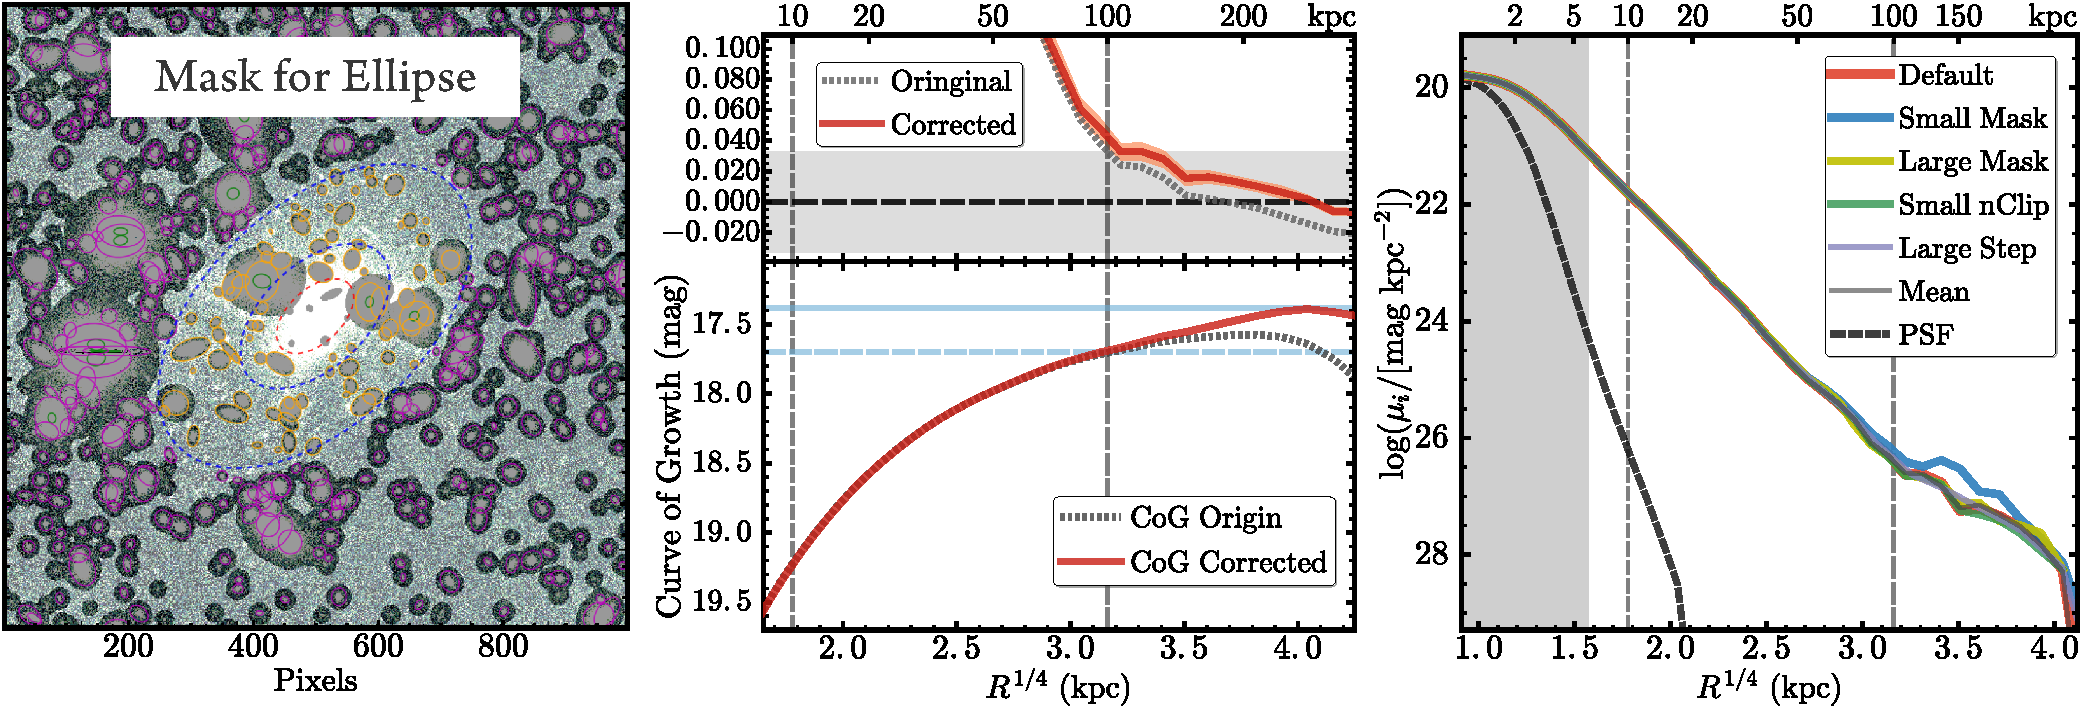
\includegraphics[width=\textwidth]{fig/redbcg_ellipse_tech}
        \caption{
            \textbf{Left:} Example of the object-mask built for the \texttt{Ellipse}
            run for a typical massive galaxy in the sample. 
            All the shaded regions are masked out. 
            The three dash lines (red, inner one and two blue ones) around the target 
            at the center outlines the three radius we defined using the flux radius 
            of the target.  
            We increase the mask size for objects detected in different regions 
            separated by these apertures (which are outlined by solid, elliptical 
            apertures with different colors) using slightly different criteria.~~
            \textbf{Middle:}: The zoom-in intensity profile around very low intensity 
            value (top panel), and the curve-of-growth of the enclosed magnitude 
            (bottom panel) of the example galaxy.  
            To highlight the importance of background correction, we show the profiles 
            using both images with (red, solid line) and without (black, dotted line) 
            background correction. 
            On the top panel, besides the horizontal line that highlights the zero flux 
            level, we also show the uncertainty of the sky background estimate using 
            the grey-shaded region.  
            On the bottom panel, two horizontal lines indicate the magnitudes 
            corresponding to total flux (solid) and flux within 100 kpc (dash).~~
            \textbf{Right:} compares the 1-D surface brightness profiles for the same 
            example galaxy using different masks 
            (smaller masking region: red, dash line; larger masks: blue, dash line), 
            or different \texttt{Ellipse} configurations
            (more aggressive pixel-clipping: cyan, dash line; 
             larger step in radius: green, dash line; 
             using mean flux along the isophote instead of median: purple, dash line)
            with the default one (black, solid line).
            }
        \label{fig:ell_tech}
    \end{figure*}
%% ------------------------------------------------------------------------------------ %% 

%% ------------------------------------------------------------------------------------ %% 
\section{B. Estimate average {$M_{\star}/L_{\star}$} using \texttt{iSEDFit}} 
    \label{app:sed} 

%% ------------------------------------------------------------------------------------ %% 
    \begin{figure*}
        \begin{center}
        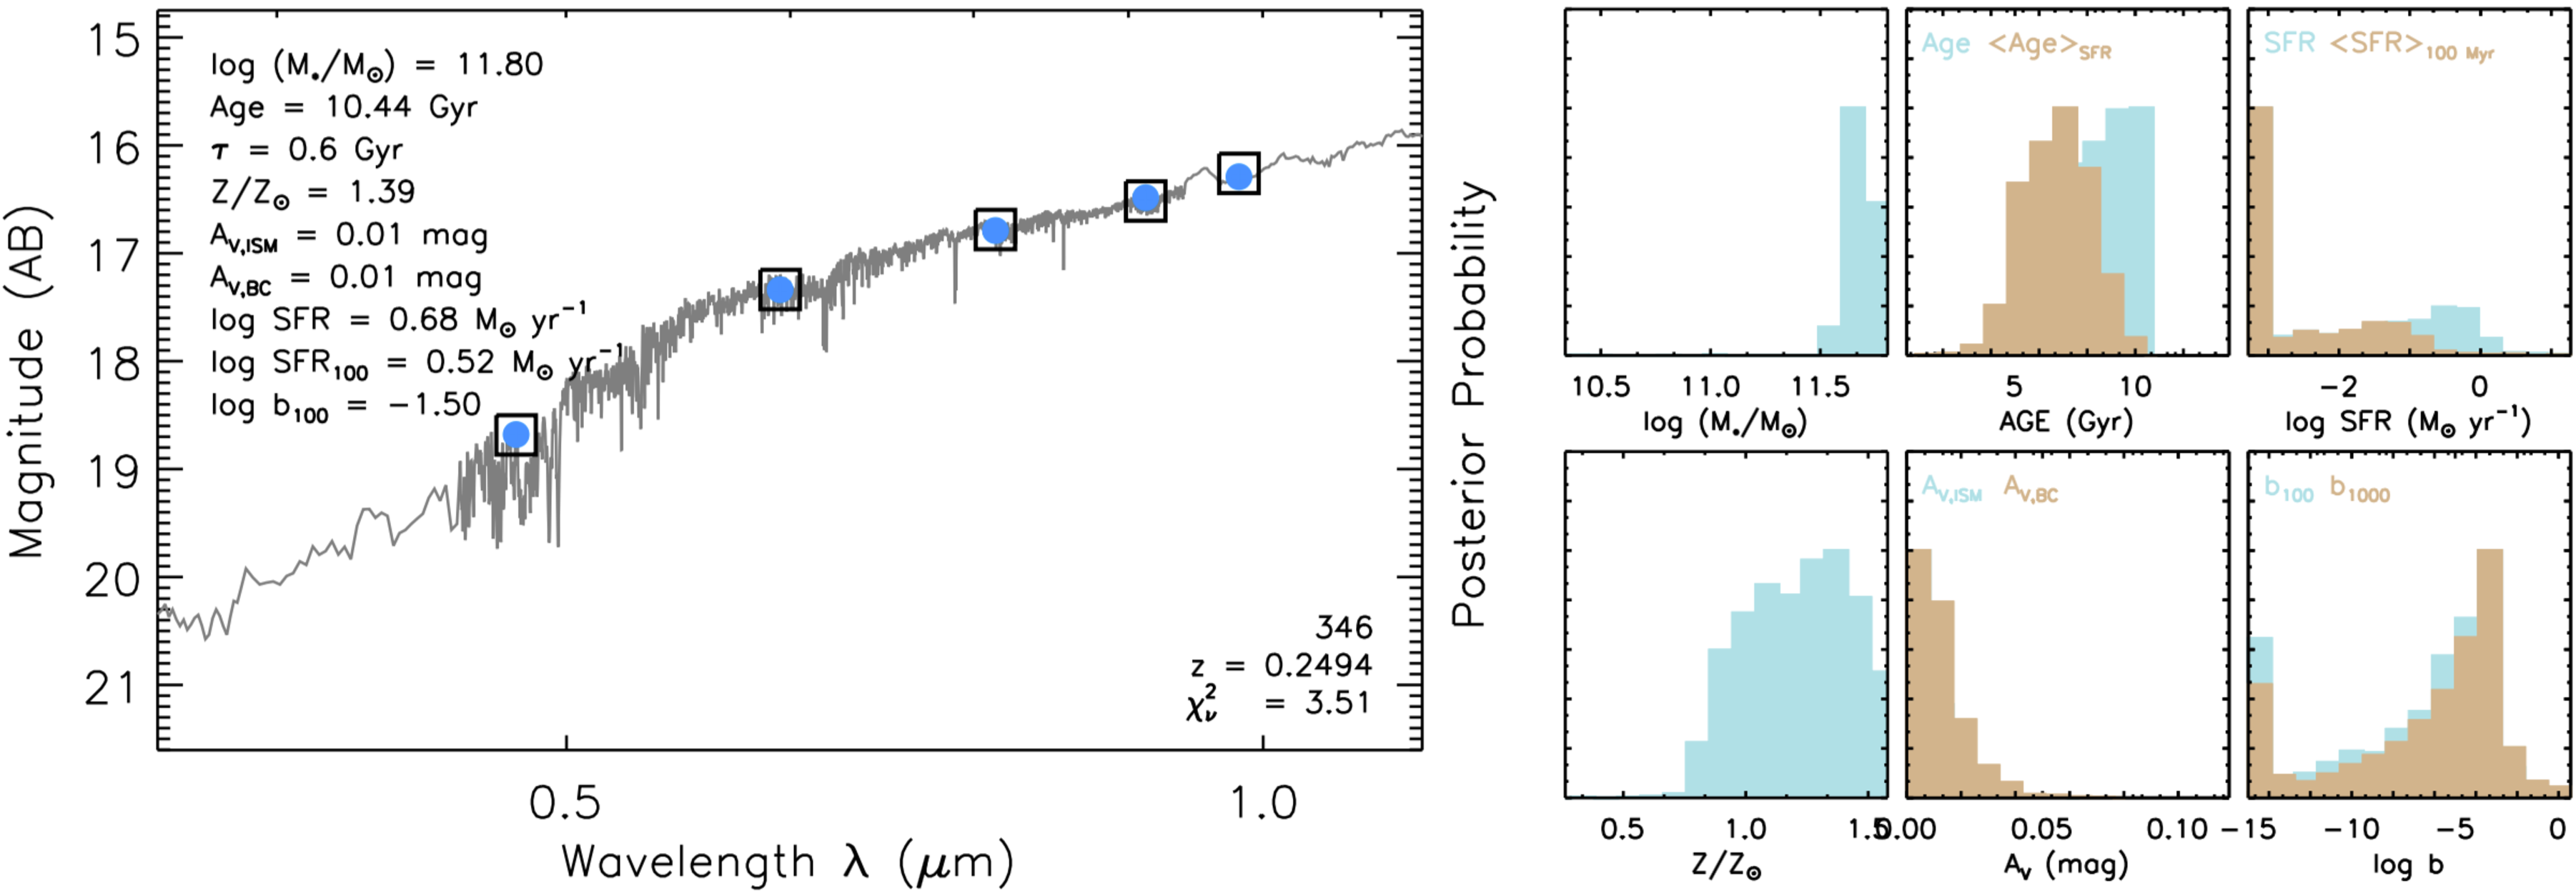
\includegraphics[width=\textwidth]{fig/redbcg_isedfit_example.pdf}
        \caption{
            \textbf{Left:} Example of output figure from \texttt{iSEDFit} that shows 
            the SED fitting results. 
            The open-boxes show the observed fluxes in 5-band, and the solid, blue-dots
            show the best-fitted results, along with the high-resolution spectrum for
            this model reconstructed using the synthetic spectra from \texttt{FSPS}. 
            Top-left corner shows the best-fit stellar population parameters, and 
            bottom-right corner shows the ID, redshift of this object, and reduced 
            $\chi^2$ of the best-fit model.~~~
            \textbf{Right:} the Posterior distributions of a few key parameters.
            From top-left to bottom right are: 
            1) stellar mass (\logms{}); 
            2) age of the population (mass and star-formation rate weighted) in Gyr; 
            3) star formation rate ($\log\ \mathrm{SFR}\ (M_{\odot}/\mathrm{yr})$; 
            instant one and the one averaged over the previous 100 Myr; 
            4) stellar metallicity ($\mathrm{Z}/\mathrm{Z}_{\odot}$); 
            5) dust extinction ($\mathrm{A}_V$ in mag);
            6) birthrate parameter ($\log\ b$; averaged over previous 100 and 1000 Myr).
            }
        \label{fig:ised}
        \end{center}
    \end{figure*}
%% ------------------------------------------------------------------------------------ %% 

%% ------------------------------------------------------------------------------------ %% 
    \begin{figure*}
        \begin{center}
        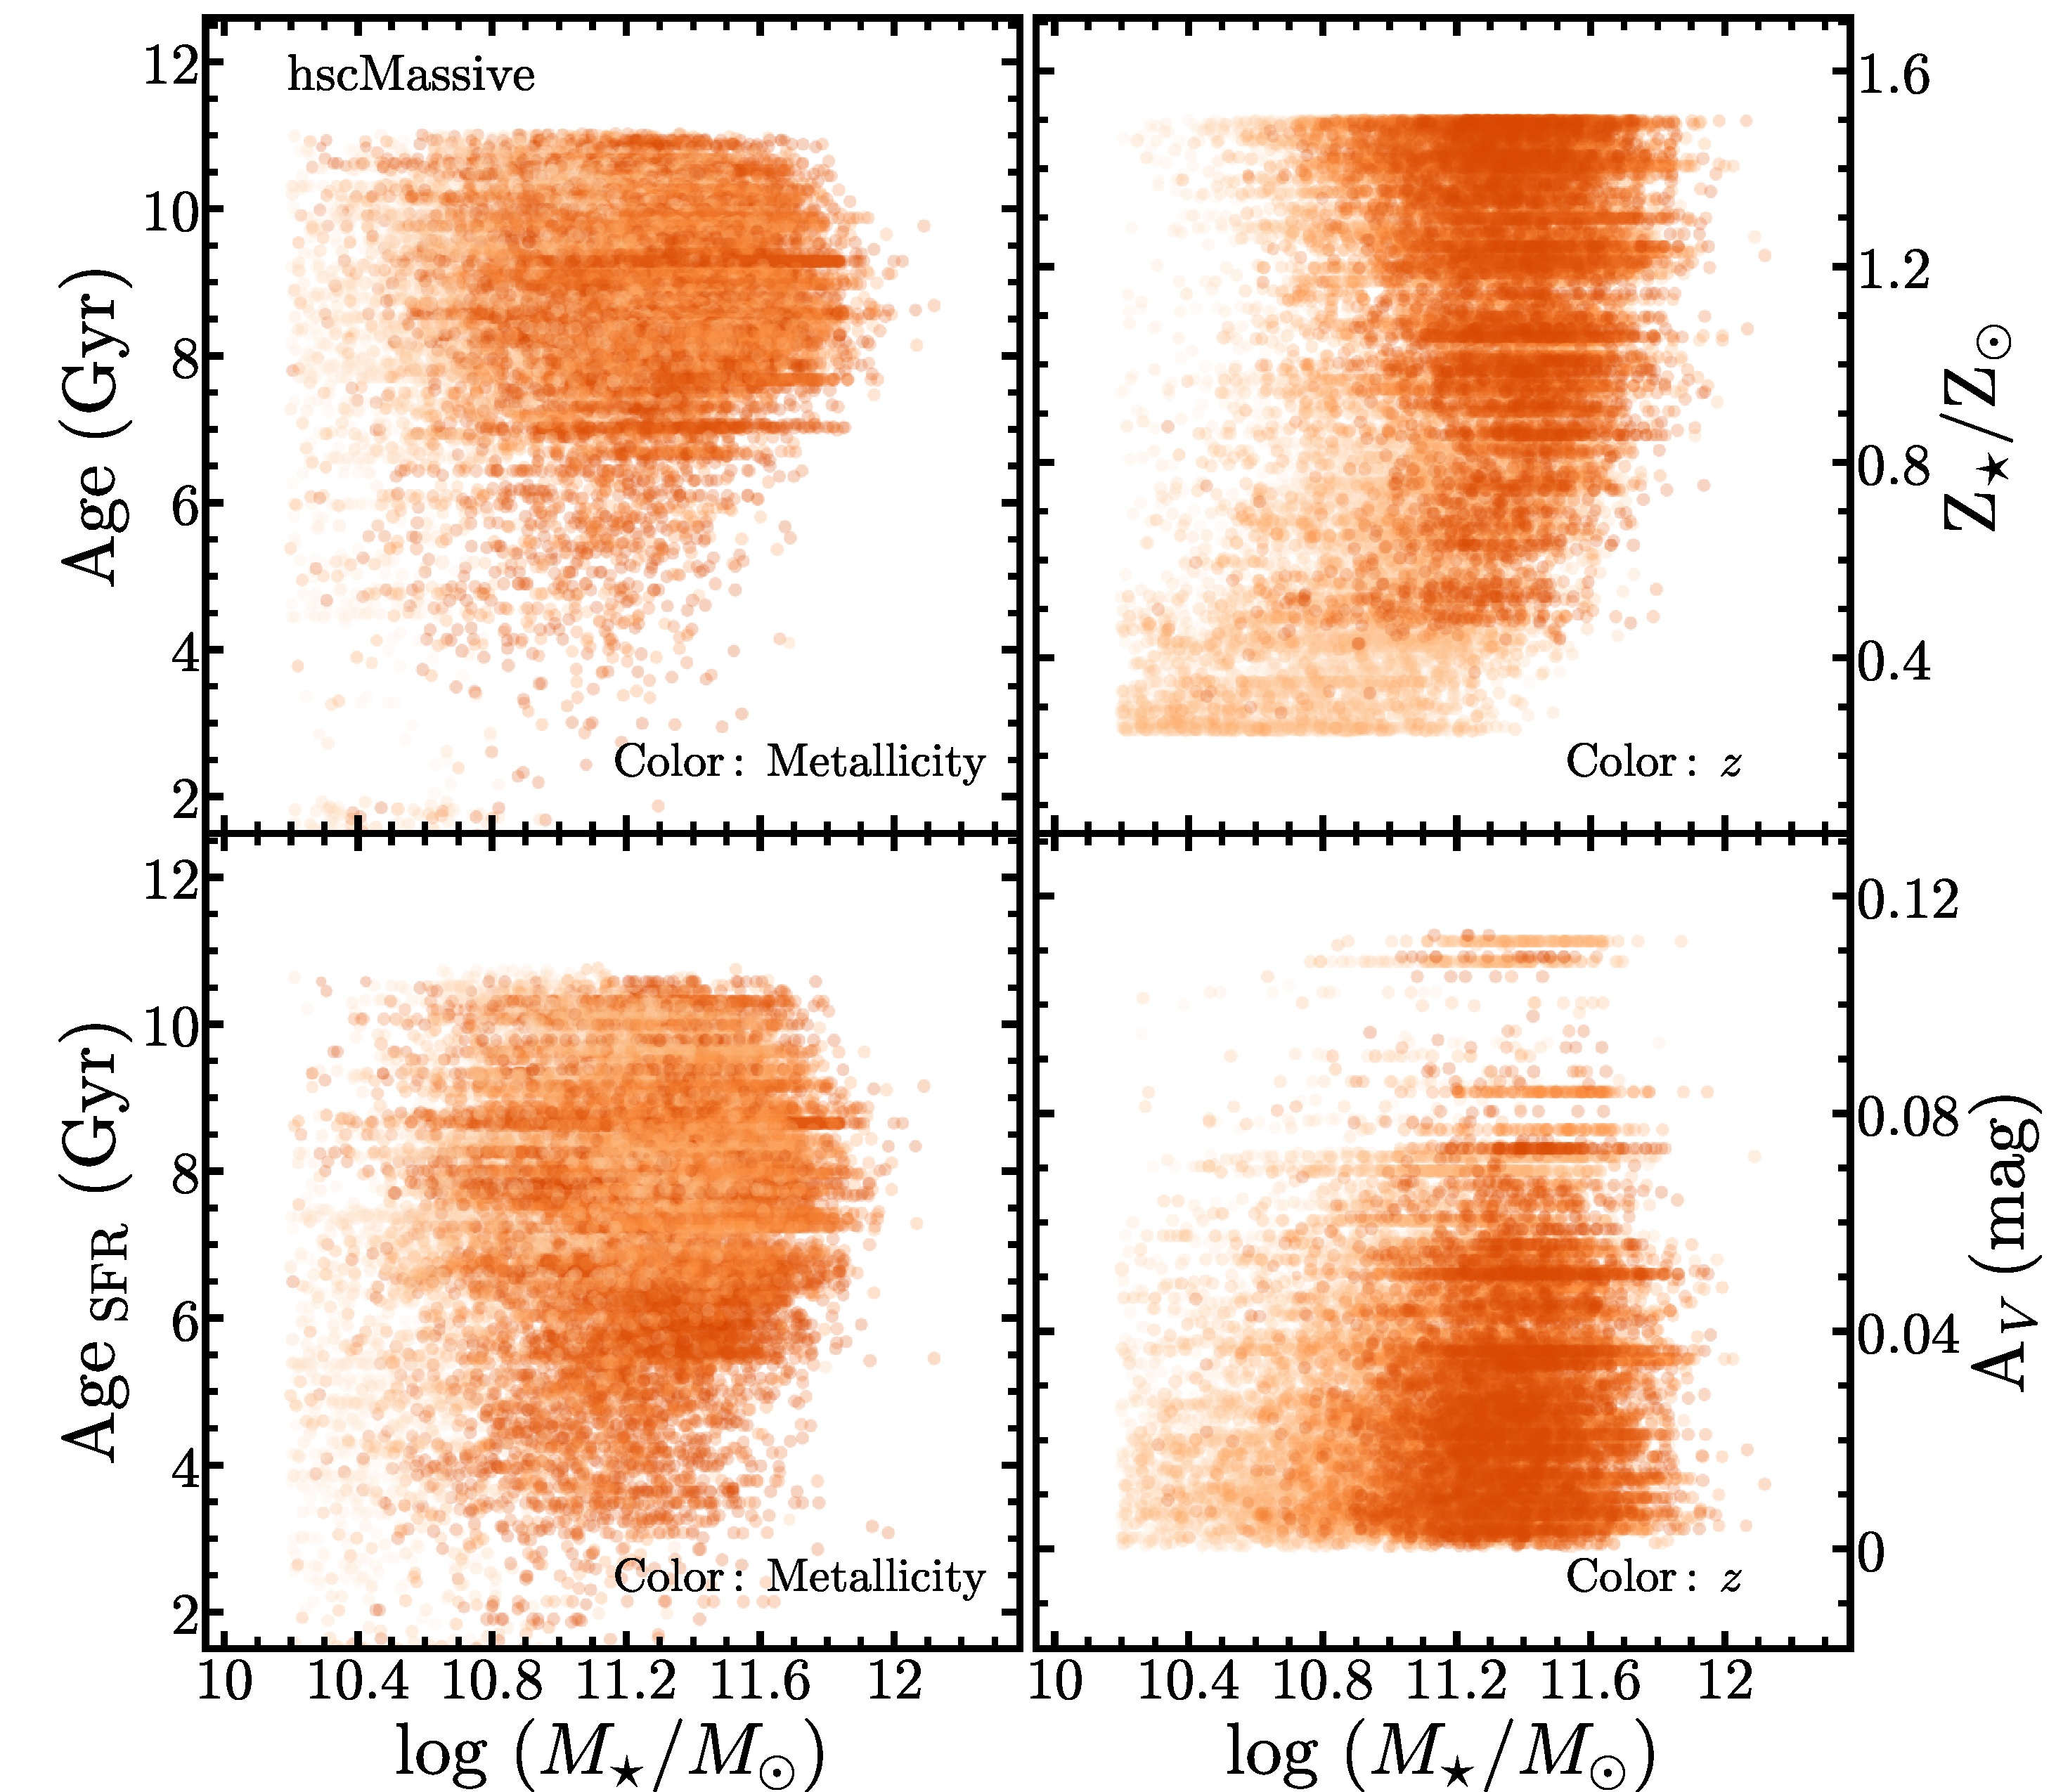
\includegraphics[width=12cm]{fig/redbcg_isedfit_2.pdf}
        \caption{
            Relationships between \mstar{} and key stellar population parameters from 
            \texttt{iSEDfit}. 
            The four stellar population properties are: 
            1) \textbf{Top-left}: \mstar{}-weighted stellar population age in Gyr; 
            2) \textbf{Bottom-left}: SFR-weighted age in Gyr; 
            3) \textbf{Top-right}: \mstar{}-weighted stellar metallicity in unit of 
            Solar value;
            4) \textbf{bottom-right}: dust extinction value in $V$-band.
            As expected, most of the HSC massive galaxies are old, metal-rich, and 
            dust-free. 
            }
        \label{fig:ised_2}
        \end{center}
    \end{figure*}
%% ------------------------------------------------------------------------------------ %% 

%% ------------------------------------------------------------------------------------ %% 
    \begin{figure}
        \begin{center}
        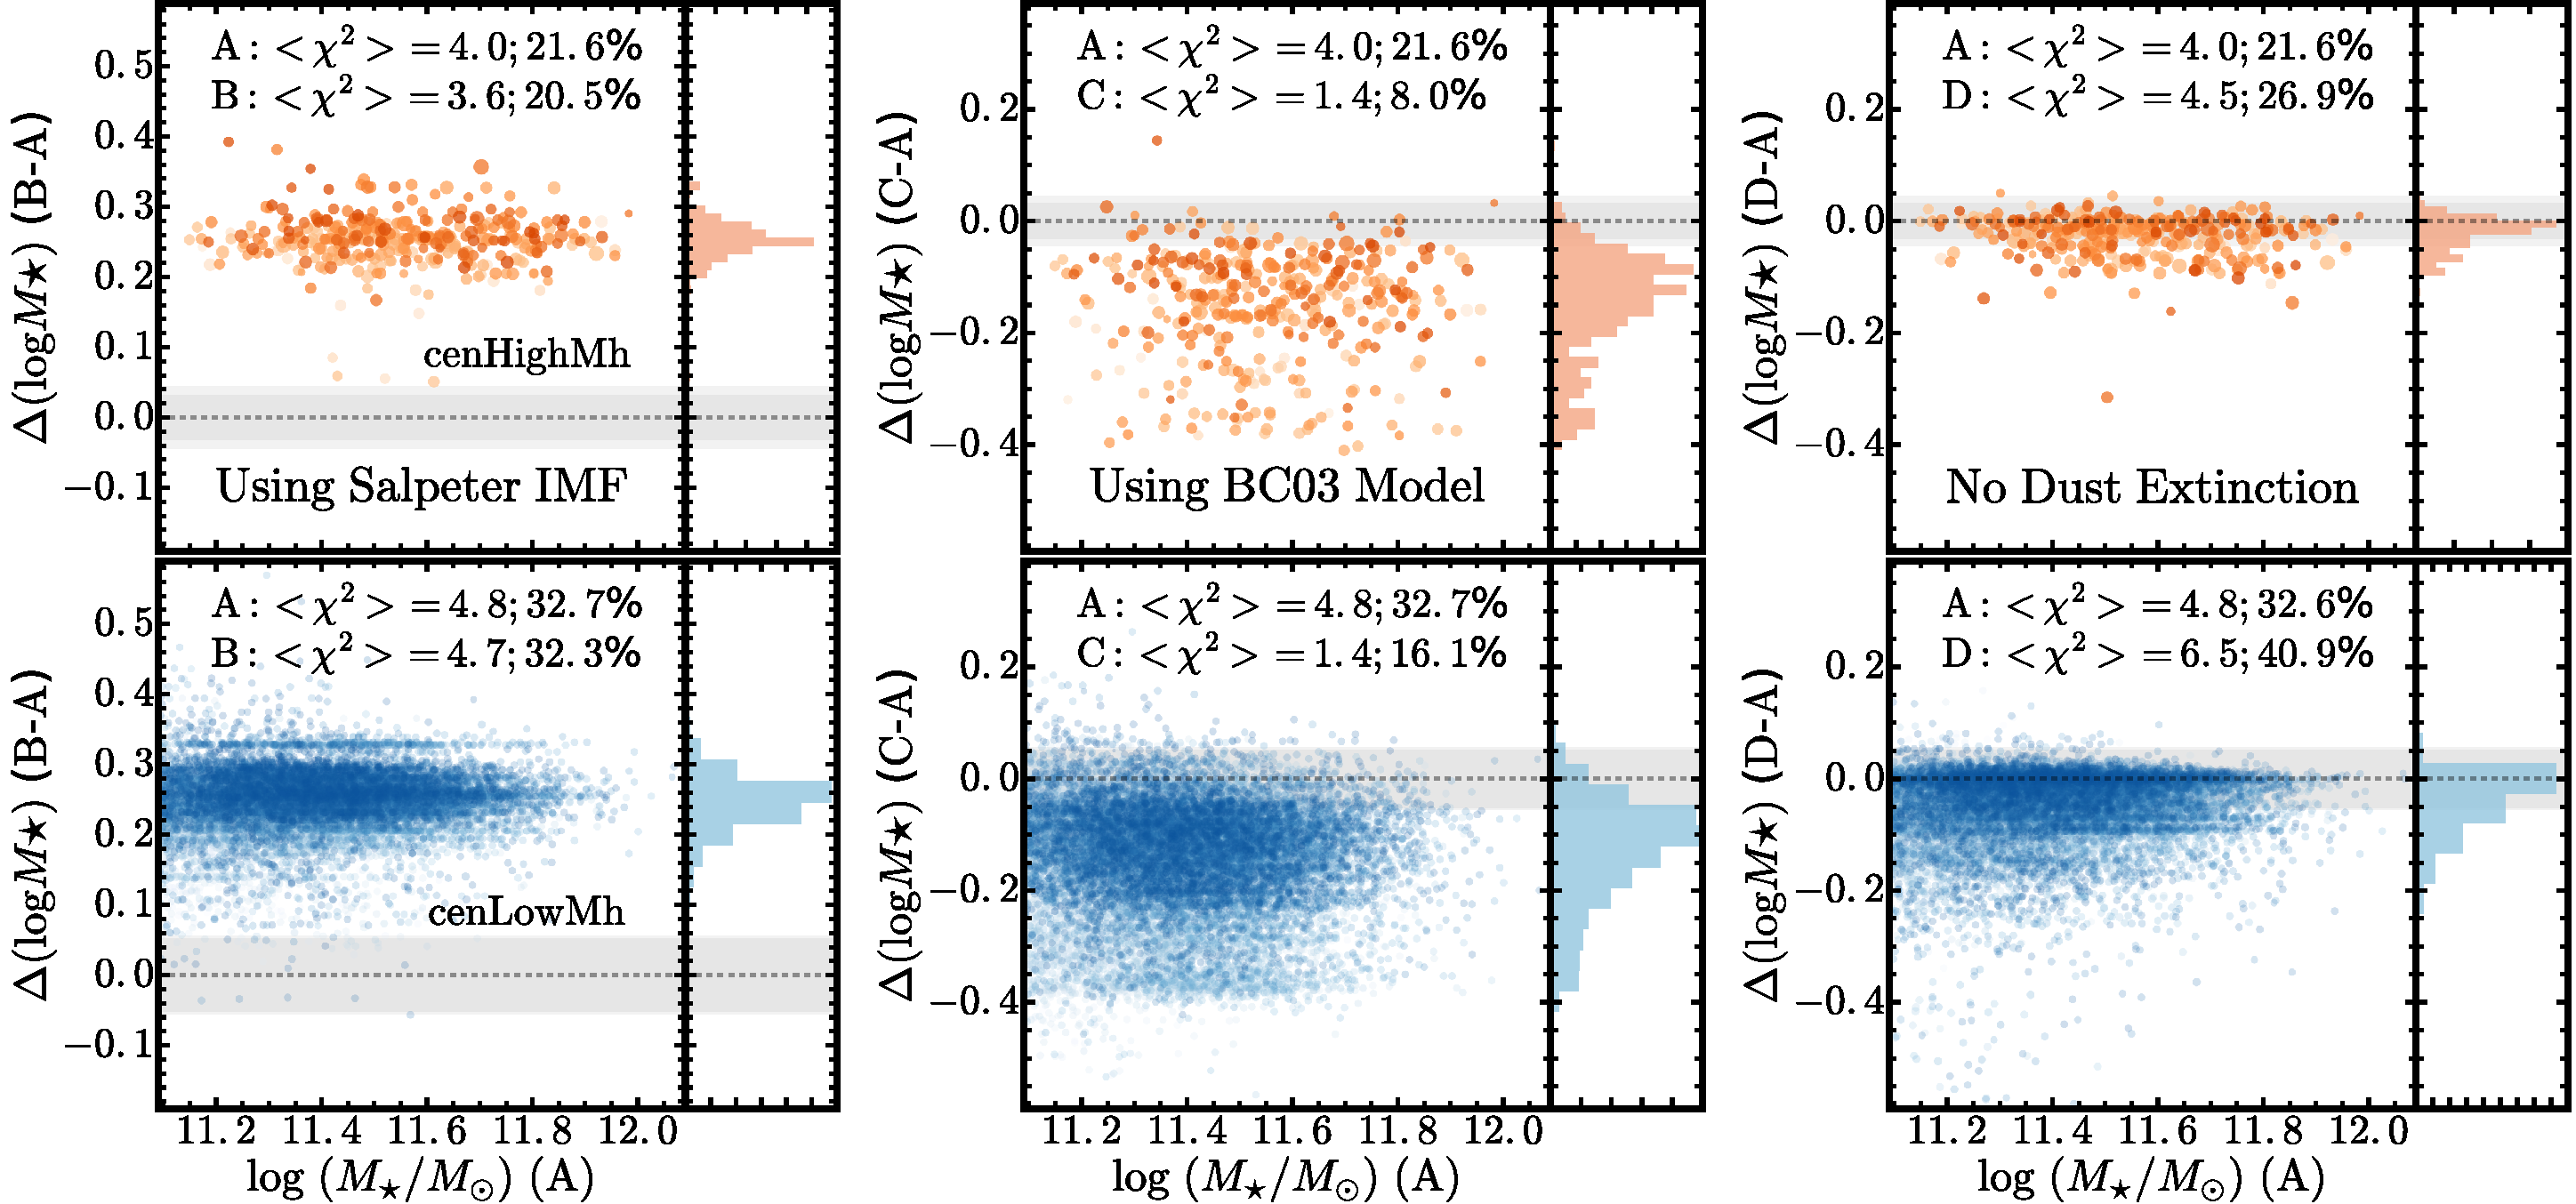
\includegraphics[width=\columnwidth]{fig/redbcg_isedfit_3.pdf}
        \caption{
            Comparisons of \mstar{} estimated by \texttt{iSEDFit} using different
            model assumptions. 
            In each figure, we plot the \mstar{} from the default model against the
            differences with other models. 
            The four models involved are labeled as: 
            (A): Default model; 
            (B): Using the Salpeter IMF instead of the Chabrier one 
                (\textbf{Top panel});
            (C): Using the BC03 synthetic population model instead of the FSPS one
                (\textbf{Middle panel});
            (D): No dust extinction (\textbf{Bottom panel}). 
            On each panel, the grey shaded region highlights the typical uncertainty 
            of the $\log($\logms{}$)$.            
            For each pair of models, we highlight their median $\chi^{2}$ values and 
            the fraction of galaxies with $\chi^{2} > 10.0$ at the top. 
            On each panel, we also show the histograms of the \mstar{}-differences on 
            the right side.
            }
        \label{fig:ised_3}
        \end{center}
    \end{figure}
%% ------------------------------------------------------------------------------------ %% 

%% ------------------------------------------------------------------------------------ %% 
 
    In Section~\ref{ssec:isedfit}, we briefly explain the SED fitting procedure and 
    the priors used.   
    In Fig~\ref{fig:ised_1}, we show an example of the \texttt{iSEDFit} output by 
    visualizing the 5-band HSC SED on top of the best-fit model along with the PDF 
    of the key parameters.
     
    Although we only use the best-fit \m2l{} in this work, it is necessary to make 
    sure the model is reasonable. 
    We show the relations between \mstar{} and a few key stellar population parameters 
    derived by \texttt{iSEDFit} in Fig~\ref{fig:ised_2}. 
    Degeneracies among these parameters are inevitable based on only five broad-band
    photometry, but as expected, most massive galaxies show old stellar age, high
    stellar metallicity ($1.5 \times Z_{\odot}$ is the highest metallicity allowed by 
    the adopted \texttt{FSPS} SSP models), and low dust extinction.
   
    Meanwhile, \mstar{} measurement based on SED fitting heavily depends on the 
    adopted SSP model, the form of IMF, dust extinction law, and details in 
    the assumption of SFH (e.g.\ \citealt{Bernardi2016b}). 
    For massive galaxies in this sample, the form of the SFH\footnote{We choose 
    to use the delayed-$\tau$ model for SFH; we adopt flat distribution between 
    0.5 to 14.0 Gyrs as the prior for the look-back time when the star formation 
    turned on. 
    The exponential delayed time-scale ($\tau$) is allowed to change between 
    0.1 to 3.0 with equal probability}, the contribution from random star 
    burst\footnote{The chance of random star burst is set at 0.2 for every 2 Gyrs. 
    The duration of the star burst is draw from a logarithmic distribution 
    between 0.03 to 0.3 Gyr; and the mass fraction formed in the burst is from 
    a logarithmic distribution between 0.01 and 1.0.} rarely affect the \mstar{}. 
    But he choices of SSP model, IMF, and dust extinction do systematically impact
    the estimates of \mstar{}, and therefore we look into this with a few 
    additional tests (see Fig~\ref{fig:ised_3}):

    \begin{enumerate}

        \item Choosing the \citet{Salpeter1955} IMF results in systematically 
            higher \mstar{} (on average $+0.25$ dex of \logms{}) for these massive 
            galaxies (top panel).
            Although there are multiple lines of evidence that favor Salpeter 
            or even more ``bottom-heavy'' IMF in massive galaxies 
            (e.g.\ \citealt{Conroy2012}; \citealt{Cappellari2012}), we still 
            present the main results using Chabrier IMF to accommodate galaxies 
            with lower \mstar{} in the sample, and to be as consistent as possible 
            with previous works.  
            This choice of IMF does not change the main results qualitatively. 

        \item \mstar{} based on the \texttt{BC03} models are systematically lower 
            than the ones based on \texttt{FSPS+MILES} models (middle panel)
            The difference shows a large scatter, and can be as large as 0.4 dex,
            although it is not \mstar{}-dependent. 
            The \texttt{BC03} results show better average ${\chi}^2$ than the 
            \texttt{FSPS} ones. 
            This relates to the higher upper-limit of stellar metallicity 
            ($2 \times \mathrm{Z}_{\odot}$) allowed by the \texttt{BC03} model, 
            which help fits the shape of the SED in the red-end slightly better.  
            However, the \texttt{BC03} results also show puzzlingly low stellar 
            ages ($< 3$--4 Gyrs) for these massive, red galaxies. 
            This could also lead to underestimated \m2l{} values.
            It is worth noting that, both \texttt{FSPS} and \texttt{BC03} 
            models still have difficulties recovering SED at the very red-end 
            (between $z$ and $y$-band), and reproducing the optical color-color 
            relations for red-sequence galaxies (e.g.\ \citealt{MIUSCAT2}).
            In this work, we decide to keep using the \texttt{FSPS+MILES} model as 
            the fiducial one.  
            Using results based on \texttt{BC03} model will not change any of our 
            conclusions here.
            
        \item On the bottom panel of Fig~\ref{fig:ised_3}, we compare with the
            SED fitting results without considering the dust extinction. 
            This choice leads to slightly smaller \mstar{} values as expected. 
            Its impact becomes slightly larger at lower \mstar{} end. 
            It will not change any of our conclusions here.
          
    \end{enumerate}
%% ------------------------------------------------------------------------------------ %% 
     
%% ------------------------------------------------------------------------------------ %% 
%% Table.1 
%% ------------------------------------------------------------------------------------ %% 
\clearpage
\begin{deluxetable}{c ccc cc cc}[b!]
\tabletypesize{\scriptsize}
\tablewidth{0pt}
\tablecolumns{8}
\tablenum{1}
\tablecaption{Average \mden{} Profiles of Massive Galaxies in Different Stellar Mass Bins}
%% ------------------------------------------------------------------------------------ %% 
\tablehead{
    \colhead{Radius} & 
    \multicolumn{3}{c}{[\mden{}]; Combined samples} &
    \multicolumn{2}{c}{[\mden{}]; $M_{\star,100\ \mathrm{kpc}}$-matched} &
    \multicolumn{2}{c}{[\mden{}]; $M_{\star,10\ \mathrm{kpc}}$-matched}
	\vspace{1.4ex}
    %------------------------------------------------------------------------------------%
    \nl 
    \colhead{kpc} & 
    \multicolumn{3}{c}{$\log (M_{\odot}/\mathrm{kpc}^2)$} &
    \multicolumn{2}{c}{$\log (M_{\odot}/\mathrm{kpc}^2)$} &
    \multicolumn{2}{c}{$\log (M_{\odot}/\mathrm{kpc}^2)$}
	\vspace{1.4ex}
    %------------------------------------------------------------------------------------%
    \nl 
    \colhead{} & 
    \colhead{$\log \frac{M_{\star,100\mathrm{kpc}}}{M_{\odot}}\in$[11.4, 11.6]} & 
    \colhead{[11.6, 11.8]} & 
    \colhead{[11.8, 12.0]}\hspace{2.0ex} & 
    \colhead{\texttt{cenHighMh}} & 
    \colhead{\texttt{cenLowMh}} & 
    \colhead{\texttt{cenHighMh}}\hspace{2.0ex} & 
    \colhead{\texttt{cenLowMh}}
    %------------------------------------------------------------------------------------%
	\vspace{1.6ex}
    %------------------------------------------------------------------------------------%
    \nl
    \colhead{    (1)} &
    \colhead{    (2)} &
    \colhead{    (3)} &
    \colhead{    (4)} &
    \colhead{    (5)} &
    \colhead{    (6)} &
    \colhead{    (7)} &
    \colhead{    (8)}
    %------------------------------------------------------------------------------------%
}
%% ------------------------------------------------------------------------------------ %% 
\startdata
%% ------------------------------------------------------------------------------------ %% 

0.0 & $ 9.23\substack{+0.00 \\ -0.00}$ &$ 9.31\substack{+0.00 \\ -0.01}$ &$ 9.32\substack{+0.01 \\ -0.01}$ &$ 9.31\substack{+0.02 \\ -0.02}$ &$ 9.34\substack{+0.01 \\ -0.01}$ &$ 9.31\substack{+0.02 \\ -0.02}$ &$ 9.34\substack{+0.02 \\ -0.02}$ \\
 0.6 & $ 9.20\substack{+0.00 \\ -0.00}$ &$ 9.28\substack{+0.00 \\ -0.01}$ &$ 9.29\substack{+0.01 \\ -0.01}$ &$ 9.27\substack{+0.02 \\ -0.02}$ &$ 9.31\substack{+0.01 \\ -0.01}$ &$ 9.28\substack{+0.02 \\ -0.02}$ &$ 9.31\substack{+0.02 \\ -0.02}$ \\
 1.0 & $ 9.16\substack{+0.00 \\ -0.00}$ &$ 9.24\substack{+0.00 \\ -0.00}$ &$ 9.26\substack{+0.01 \\ -0.01}$ &$ 9.24\substack{+0.02 \\ -0.02}$ &$ 9.27\substack{+0.01 \\ -0.01}$ &$ 9.25\substack{+0.02 \\ -0.02}$ &$ 9.27\substack{+0.02 \\ -0.02}$ \\
 1.4 & $ 9.12\substack{+0.00 \\ -0.00}$ &$ 9.20\substack{+0.00 \\ -0.00}$ &$ 9.23\substack{+0.01 \\ -0.01}$ &$ 9.20\substack{+0.02 \\ -0.02}$ &$ 9.23\substack{+0.01 \\ -0.01}$ &$ 9.21\substack{+0.02 \\ -0.01}$ &$ 9.23\substack{+0.02 \\ -0.01}$ \\
 1.7 & $ 9.06\substack{+0.00 \\ -0.00}$ &$ 9.15\substack{+0.00 \\ -0.00}$ &$ 9.19\substack{+0.01 \\ -0.01}$ &$ 9.15\substack{+0.02 \\ -0.02}$ &$ 9.19\substack{+0.01 \\ -0.01}$ &$ 9.16\substack{+0.01 \\ -0.01}$ &$ 9.18\substack{+0.01 \\ -0.01}$ \\
 2.0 & $ 9.00\substack{+0.00 \\ -0.00}$ &$ 9.10\substack{+0.00 \\ -0.00}$ &$ 9.15\substack{+0.01 \\ -0.01}$ &$ 9.09\substack{+0.01 \\ -0.02}$ &$ 9.13\substack{+0.01 \\ -0.01}$ &$ 9.11\substack{+0.01 \\ -0.01}$ &$ 9.12\substack{+0.01 \\ -0.01}$ \\
 2.4 & $ 8.93\substack{+0.00 \\ -0.00}$ &$ 9.03\substack{+0.00 \\ -0.00}$ &$ 9.09\substack{+0.01 \\ -0.01}$ &$ 9.03\substack{+0.02 \\ -0.02}$ &$ 9.07\substack{+0.01 \\ -0.01}$ &$ 9.05\substack{+0.01 \\ -0.01}$ &$ 9.05\substack{+0.01 \\ -0.01}$ \\
 2.7 & $ 8.87\substack{+0.00 \\ -0.00}$ &$ 8.97\substack{+0.00 \\ -0.00}$ &$ 9.04\substack{+0.01 \\ -0.01}$ &$ 8.97\substack{+0.01 \\ -0.01}$ &$ 9.01\substack{+0.01 \\ -0.01}$ &$ 9.00\substack{+0.01 \\ -0.01}$ &$ 8.99\substack{+0.01 \\ -0.01}$ \\
 3.0 & $ 8.80\substack{+0.00 \\ -0.00}$ &$ 8.90\substack{+0.00 \\ -0.00}$ &$ 8.98\substack{+0.01 \\ -0.01}$ &$ 8.90\substack{+0.01 \\ -0.01}$ &$ 8.95\substack{+0.01 \\ -0.01}$ &$ 8.93\substack{+0.01 \\ -0.01}$ &$ 8.92\substack{+0.01 \\ -0.01}$ \\
 3.4 & $ 8.72\substack{+0.00 \\ -0.00}$ &$ 8.83\substack{+0.00 \\ -0.00}$ &$ 8.92\substack{+0.01 \\ -0.01}$ &$ 8.83\substack{+0.01 \\ -0.01}$ &$ 8.88\substack{+0.01 \\ -0.01}$ &$ 8.86\substack{+0.01 \\ -0.01}$ &$ 8.85\substack{+0.01 \\ -0.01}$ \\
 3.7 & $ 8.66\substack{+0.00 \\ -0.00}$ &$ 8.78\substack{+0.00 \\ -0.00}$ &$ 8.87\substack{+0.01 \\ -0.01}$ &$ 8.78\substack{+0.01 \\ -0.01}$ &$ 8.83\substack{+0.01 \\ -0.01}$ &$ 8.81\substack{+0.01 \\ -0.01}$ &$ 8.79\substack{+0.01 \\ -0.01}$ \\
 4.1 & $ 8.60\substack{+0.00 \\ -0.00}$ &$ 8.72\substack{+0.00 \\ -0.00}$ &$ 8.82\substack{+0.01 \\ -0.01}$ &$ 8.72\substack{+0.01 \\ -0.01}$ &$ 8.77\substack{+0.01 \\ -0.01}$ &$ 8.76\substack{+0.01 \\ -0.01}$ &$ 8.73\substack{+0.01 \\ -0.01}$ \\
 4.4 & $ 8.54\substack{+0.00 \\ -0.00}$ &$ 8.66\substack{+0.00 \\ -0.00}$ &$ 8.77\substack{+0.01 \\ -0.01}$ &$ 8.66\substack{+0.01 \\ -0.01}$ &$ 8.72\substack{+0.01 \\ -0.01}$ &$ 8.70\substack{+0.01 \\ -0.01}$ &$ 8.67\substack{+0.01 \\ -0.01}$ \\
 4.8 & $ 8.48\substack{+0.00 \\ -0.00}$ &$ 8.60\substack{+0.00 \\ -0.00}$ &$ 8.71\substack{+0.01 \\ -0.01}$ &$ 8.60\substack{+0.01 \\ -0.01}$ &$ 8.66\substack{+0.01 \\ -0.01}$ &$ 8.65\substack{+0.01 \\ -0.01}$ &$ 8.61\substack{+0.01 \\ -0.01}$ \\
 6.2 & $ 8.26\substack{+0.00 \\ -0.00}$ &$ 8.40\substack{+0.00 \\ -0.00}$ &$ 8.53\substack{+0.01 \\ -0.01}$ &$ 8.41\substack{+0.01 \\ -0.01}$ &$ 8.46\substack{+0.01 \\ -0.01}$ &$ 8.46\substack{+0.02 \\ -0.02}$ &$ 8.40\substack{+0.02 \\ -0.02}$ \\
 7.6 & $ 8.09\substack{+0.00 \\ -0.00}$ &$ 8.24\substack{+0.00 \\ -0.00}$ &$ 8.39\substack{+0.01 \\ -0.01}$ &$ 8.27\substack{+0.01 \\ -0.01}$ &$ 8.31\substack{+0.01 \\ -0.01}$ &$ 8.31\substack{+0.02 \\ -0.02}$ &$ 8.23\substack{+0.02 \\ -0.02}$ \\
 9.0 & $ 7.95\substack{+0.00 \\ -0.00}$ &$ 8.10\substack{+0.00 \\ -0.00}$ &$ 8.27\substack{+0.01 \\ -0.01}$ &$ 8.14\substack{+0.02 \\ -0.02}$ &$ 8.18\substack{+0.01 \\ -0.01}$ &$ 8.19\substack{+0.02 \\ -0.02}$ &$ 8.09\substack{+0.02 \\ -0.02}$ \\
10.3 & $ 7.82\substack{+0.00 \\ -0.00}$ &$ 7.99\substack{+0.00 \\ -0.00}$ &$ 8.16\substack{+0.01 \\ -0.01}$ &$ 8.03\substack{+0.02 \\ -0.01}$ &$ 8.06\substack{+0.01 \\ -0.01}$ &$ 8.09\substack{+0.02 \\ -0.02}$ &$ 7.97\substack{+0.02 \\ -0.02}$ \\
11.7 & $ 7.70\substack{+0.00 \\ -0.00}$ &$ 7.88\substack{+0.00 \\ -0.00}$ &$ 8.06\substack{+0.01 \\ -0.01}$ &$ 7.93\substack{+0.02 \\ -0.02}$ &$ 7.96\substack{+0.01 \\ -0.01}$ &$ 7.99\substack{+0.02 \\ -0.02}$ &$ 7.85\substack{+0.02 \\ -0.02}$ \\
13.0 & $ 7.60\substack{+0.00 \\ -0.00}$ &$ 7.78\substack{+0.00 \\ -0.00}$ &$ 7.98\substack{+0.01 \\ -0.01}$ &$ 7.85\substack{+0.02 \\ -0.02}$ &$ 7.87\substack{+0.01 \\ -0.01}$ &$ 7.90\substack{+0.02 \\ -0.02}$ &$ 7.75\substack{+0.02 \\ -0.02}$ \\
14.5 & $ 7.50\substack{+0.00 \\ -0.00}$ &$ 7.69\substack{+0.00 \\ -0.00}$ &$ 7.90\substack{+0.01 \\ -0.01}$ &$ 7.76\substack{+0.02 \\ -0.02}$ &$ 7.78\substack{+0.01 \\ -0.01}$ &$ 7.82\substack{+0.02 \\ -0.02}$ &$ 7.65\substack{+0.02 \\ -0.02}$ \\
16.0 & $ 7.39\substack{+0.00 \\ -0.00}$ &$ 7.60\substack{+0.00 \\ -0.00}$ &$ 7.82\substack{+0.01 \\ -0.01}$ &$ 7.68\substack{+0.02 \\ -0.02}$ &$ 7.69\substack{+0.01 \\ -0.01}$ &$ 7.74\substack{+0.02 \\ -0.03}$ &$ 7.56\substack{+0.02 \\ -0.03}$ \\
17.3 & $ 7.31\substack{+0.00 \\ -0.00}$ &$ 7.52\substack{+0.00 \\ -0.00}$ &$ 7.76\substack{+0.01 \\ -0.01}$ &$ 7.61\substack{+0.02 \\ -0.02}$ &$ 7.62\substack{+0.01 \\ -0.01}$ &$ 7.67\substack{+0.03 \\ -0.03}$ &$ 7.48\substack{+0.03 \\ -0.03}$ \\
18.7 & $ 7.23\substack{+0.00 \\ -0.00}$ &$ 7.45\substack{+0.00 \\ -0.00}$ &$ 7.69\substack{+0.01 \\ -0.01}$ &$ 7.55\substack{+0.02 \\ -0.02}$ &$ 7.55\substack{+0.01 \\ -0.01}$ &$ 7.61\substack{+0.03 \\ -0.03}$ &$ 7.40\substack{+0.03 \\ -0.03}$ \\
22.6 & $ 7.02\substack{+0.00 \\ -0.00}$ &$ 7.27\substack{+0.00 \\ -0.00}$ &$ 7.54\substack{+0.01 \\ -0.01}$ &$ 7.38\substack{+0.02 \\ -0.02}$ &$ 7.37\substack{+0.01 \\ -0.01}$ &$ 7.45\substack{+0.03 \\ -0.03}$ &$ 7.21\substack{+0.03 \\ -0.03}$ \\
26.1 & $ 6.86\substack{+0.00 \\ -0.00}$ &$ 7.12\substack{+0.00 \\ -0.00}$ &$ 7.41\substack{+0.01 \\ -0.01}$ &$ 7.25\substack{+0.02 \\ -0.02}$ &$ 7.24\substack{+0.01 \\ -0.01}$ &$ 7.32\substack{+0.03 \\ -0.03}$ &$ 7.05\substack{+0.03 \\ -0.03}$ \\
30.0 & $ 6.70\substack{+0.00 \\ -0.00}$ &$ 6.98\substack{+0.00 \\ -0.00}$ &$ 7.29\substack{+0.01 \\ -0.01}$ &$ 7.13\substack{+0.03 \\ -0.02}$ &$ 7.10\substack{+0.01 \\ -0.01}$ &$ 7.20\substack{+0.03 \\ -0.04}$ &$ 6.90\substack{+0.03 \\ -0.04}$ \\
33.7 & $ 6.55\substack{+0.00 \\ -0.00}$ &$ 6.85\substack{+0.01 \\ -0.01}$ &$ 7.18\substack{+0.01 \\ -0.01}$ &$ 7.01\substack{+0.03 \\ -0.03}$ &$ 6.98\substack{+0.01 \\ -0.01}$ &$ 7.09\substack{+0.03 \\ -0.03}$ &$ 6.76\substack{+0.03 \\ -0.03}$ \\
37.8 & $ 6.41\substack{+0.00 \\ -0.00}$ &$ 6.72\substack{+0.01 \\ -0.01}$ &$ 7.07\substack{+0.01 \\ -0.01}$ &$ 6.90\substack{+0.03 \\ -0.03}$ &$ 6.85\substack{+0.01 \\ -0.01}$ &$ 6.98\substack{+0.04 \\ -0.04}$ &$ 6.63\substack{+0.04 \\ -0.04}$ \\
41.6 & $ 6.29\substack{+0.01 \\ -0.01}$ &$ 6.61\substack{+0.01 \\ -0.01}$ &$ 6.98\substack{+0.01 \\ -0.01}$ &$ 6.81\substack{+0.03 \\ -0.03}$ &$ 6.75\substack{+0.01 \\ -0.01}$ &$ 6.89\substack{+0.04 \\ -0.04}$ &$ 6.51\substack{+0.04 \\ -0.04}$ \\
45.7 & $ 6.17\substack{+0.01 \\ -0.01}$ &$ 6.50\substack{+0.01 \\ -0.01}$ &$ 6.88\substack{+0.01 \\ -0.01}$ &$ 6.71\substack{+0.03 \\ -0.03}$ &$ 6.64\substack{+0.01 \\ -0.01}$ &$ 6.79\substack{+0.04 \\ -0.04}$ &$ 6.39\substack{+0.04 \\ -0.04}$ \\
49.3 & $ 6.07\substack{+0.01 \\ -0.01}$ &$ 6.41\substack{+0.01 \\ -0.01}$ &$ 6.80\substack{+0.01 \\ -0.02}$ &$ 6.62\substack{+0.03 \\ -0.03}$ &$ 6.56\substack{+0.01 \\ -0.01}$ &$ 6.70\substack{+0.04 \\ -0.04}$ &$ 6.30\substack{+0.04 \\ -0.04}$ \\
53.1 & $ 5.98\substack{+0.01 \\ -0.01}$ &$ 6.33\substack{+0.01 \\ -0.01}$ &$ 6.71\substack{+0.02 \\ -0.02}$ &$ 6.55\substack{+0.03 \\ -0.03}$ &$ 6.46\substack{+0.01 \\ -0.01}$ &$ 6.64\substack{+0.04 \\ -0.04}$ &$ 6.21\substack{+0.04 \\ -0.04}$ \\
57.2 & $ 5.88\substack{+0.01 \\ -0.01}$ &$ 6.24\substack{+0.01 \\ -0.01}$ &$ 6.63\substack{+0.02 \\ -0.02}$ &$ 6.47\substack{+0.04 \\ -0.04}$ &$ 6.37\substack{+0.01 \\ -0.01}$ &$ 6.56\substack{+0.04 \\ -0.04}$ &$ 6.11\substack{+0.04 \\ -0.04}$ \\
61.5 & $ 5.79\substack{+0.01 \\ -0.01}$ &$ 6.15\substack{+0.01 \\ -0.01}$ &$ 6.55\substack{+0.02 \\ -0.02}$ &$ 6.39\substack{+0.04 \\ -0.04}$ &$ 6.29\substack{+0.01 \\ -0.01}$ &$ 6.49\substack{+0.04 \\ -0.04}$ &$ 6.03\substack{+0.04 \\ -0.04}$ \\
66.0 & $ 5.70\substack{+0.01 \\ -0.01}$ &$ 6.05\substack{+0.01 \\ -0.01}$ &$ 6.47\substack{+0.02 \\ -0.02}$ &$ 6.32\substack{+0.04 \\ -0.04}$ &$ 6.20\substack{+0.01 \\ -0.01}$ &$ 6.37\substack{+0.05 \\ -0.06}$ &$ 5.94\substack{+0.05 \\ -0.06}$ \\
69.8 & $ 5.64\substack{+0.01 \\ -0.01}$ &$ 5.98\substack{+0.01 \\ -0.01}$ &$ 6.40\substack{+0.02 \\ -0.02}$ &$ 6.25\substack{+0.04 \\ -0.04}$ &$ 6.12\substack{+0.02 \\ -0.01}$ &$ 6.35\substack{+0.04 \\ -0.05}$ &$ 5.87\substack{+0.04 \\ -0.05}$ \\
74.7 & $ 5.56\substack{+0.01 \\ -0.01}$ &$ 5.89\substack{+0.01 \\ -0.01}$ &$ 6.32\substack{+0.02 \\ -0.02}$ &$ 6.18\substack{+0.04 \\ -0.04}$ &$ 6.04\substack{+0.02 \\ -0.02}$ &$ 6.28\substack{+0.05 \\ -0.05}$ &$ 5.79\substack{+0.05 \\ -0.05}$ \\
79.9 & $ 5.49\substack{+0.01 \\ -0.01}$ &$ 5.81\substack{+0.01 \\ -0.01}$ &$ 6.24\substack{+0.02 \\ -0.02}$ &$ 6.12\substack{+0.04 \\ -0.04}$ &$ 5.96\substack{+0.02 \\ -0.02}$ &$ 6.20\substack{+0.05 \\ -0.06}$ &$ 5.72\substack{+0.05 \\ -0.06}$ \\
84.3 & $ 5.43\substack{+0.01 \\ -0.01}$ &$ 5.74\substack{+0.01 \\ -0.01}$ &$ 6.18\substack{+0.02 \\ -0.02}$ &$ 6.05\substack{+0.04 \\ -0.05}$ &$ 5.89\substack{+0.02 \\ -0.02}$ &$ 6.16\substack{+0.05 \\ -0.05}$ &$ 5.65\substack{+0.05 \\ -0.05}$ \\
88.8 & $ 5.38\substack{+0.01 \\ -0.01}$ &$ 5.67\substack{+0.01 \\ -0.01}$ &$ 6.11\substack{+0.02 \\ -0.02}$ &$ 5.99\substack{+0.05 \\ -0.06}$ &$ 5.81\substack{+0.02 \\ -0.02}$ &$ 6.08\substack{+0.05 \\ -0.06}$ &$ 5.58\substack{+0.05 \\ -0.06}$ \\
97.2 & $ 5.29\substack{+0.01 \\ -0.01}$ &$ 5.56\substack{+0.01 \\ -0.01}$ &$ 5.98\substack{+0.02 \\ -0.02}$ &$ 5.92\substack{+0.04 \\ -0.04}$ &$ 5.69\substack{+0.02 \\ -0.02}$ &$ 5.99\substack{+0.05 \\ -0.05}$ &$ 5.47\substack{+0.05 \\ -0.05}$ \\
103.6 & $ 5.21\substack{+0.01 \\ -0.01}$ &$ 5.49\substack{+0.01 \\ -0.01}$ &$ 5.89\substack{+0.03 \\ -0.03}$ &$ 5.84\substack{+0.05 \\ -0.05}$ &$ 5.62\substack{+0.02 \\ -0.02}$ &$ 5.94\substack{+0.05 \\ -0.05}$ &$ 5.39\substack{+0.05 \\ -0.05}$ \\
111.6 & $ 5.14\substack{+0.01 \\ -0.01}$ &$ 5.40\substack{+0.01 \\ -0.01}$ &$ 5.79\substack{+0.03 \\ -0.03}$ &$ 5.78\substack{+0.05 \\ -0.05}$ &$ 5.54\substack{+0.02 \\ -0.02}$ &$ 5.87\substack{+0.05 \\ -0.05}$ &$ 5.32\substack{+0.05 \\ -0.05}$ \\
117.2 & $ 5.10\substack{+0.01 \\ -0.01}$ &$ 5.36\substack{+0.01 \\ -0.01}$ &$ 5.72\substack{+0.03 \\ -0.03}$ &$ 5.72\substack{+0.05 \\ -0.05}$ &$ 5.47\substack{+0.02 \\ -0.02}$ &$ 5.82\substack{+0.05 \\ -0.05}$ &$ 5.29\substack{+0.05 \\ -0.05}$ \\
129.0 & $ 5.00\substack{+0.01 \\ -0.01}$ &$ 5.25\substack{+0.02 \\ -0.02}$ &$ 5.61\substack{+0.03 \\ -0.03}$ &$ 5.64\substack{+0.05 \\ -0.05}$ &$ 5.36\substack{+0.02 \\ -0.02}$ &$ 5.74\substack{+0.05 \\ -0.05}$ &$ 5.21\substack{+0.05 \\ -0.05}$ \\
141.7 & $ 4.89\substack{+0.02 \\ -0.02}$ &$ 5.13\substack{+0.02 \\ -0.02}$ &$ 5.49\substack{+0.03 \\ -0.03}$ &$ 5.58\substack{+0.05 \\ -0.05}$ &$ 5.23\substack{+0.03 \\ -0.03}$ &$ 5.66\substack{+0.05 \\ -0.05}$ &$ 5.09\substack{+0.05 \\ -0.05}$ \\
146.7 & $ 4.85\substack{+0.02 \\ -0.02}$ &$ 5.10\substack{+0.02 \\ -0.02}$ &$ 5.46\substack{+0.03 \\ -0.03}$ &$ 5.51\substack{+0.06 \\ -0.06}$ &$ 5.19\substack{+0.03 \\ -0.03}$ &$ 5.61\substack{+0.05 \\ -0.05}$ &$ 5.03\substack{+0.05 \\ -0.05}$ \\

%%------------------------------------------------------------------------------------ %% 
\enddata
%% ------------------------------------------------------------------------------------ %% 
\tablecomments{
    Average \mden{} profiles of massive \rbcg{} and \nbcg{} galaxies in different
    samples:\\ 
    Col.~(1) Radius along the major axis in kpc.\\
    Col.~(2) Average \mden{} profile for galaxies with 
        $11.4 \leq$\logmtot$< 11.6$ in the combined samples of \rbcg{} and \nbcg{}
        galaxies. \\ 
    Col.~(3) Average \mden{} profile of combined samples in the mass bin of 
        $11.6 \leq$\logmtot$< 11.8$. \\ 
    Col.~(4) Average \mden{} profile of combined samples in the mass bin of 
        $11.8 \leq$\logmtot$< 12.0$. \\ 
    Col.~(5) and Col.~(6) are the average \mden{} profiles of \rbcg{} and \nbcg{} galaxies
        in the \mtot{}-matched samples within $11.6 \leq$\logmtot{}$< 11.9$. \\ 
    Col.~(7) and Col.~(8) are the average \mden{} profiles of \rbcg{} and \nbcg{} galaxies 
        in the \minn{}-matched samples within $11.2 \leq$\logmtot{}$< 11.6$. \\ 
    The upper and lower uncertainties of these average profiles vial bootstrap-resampling 
    method are also displayed.
}
\label{tab:prof}
\end{deluxetable}

\clearpage
%% ------------------------------------------------------------------------------------ %% 

%% ------------------------------------------------------------------------------------ %%  
\bsp
\label{lastpage}
\end{document}
%% ------------------------------------------------------------------------------------ %% 
%%%%%%%%%%%%: End of the File %%%%%%%%%%%%
%% ------------------------------------------------------------------------------------ %% 